\chapter{Background Estimation}
\label{ch:bg_estim}

As \ttbar and $\PZ$+Jets have the same final state as the signal, they are the main sources of background in both the resolved and boosted regions of this analysis.
A schematic diagram representing the control regions used to estimate the \ttbar and $\PZ$+Jets backgrounds and the signal region is shown in Fig~\ref{fig:BkgdSchem}.
The contributions from other processes are negligible and have been estimated by counting the number of events in the simulated samples in the signal region.

\begin{figure}[htbp]
  \centering
  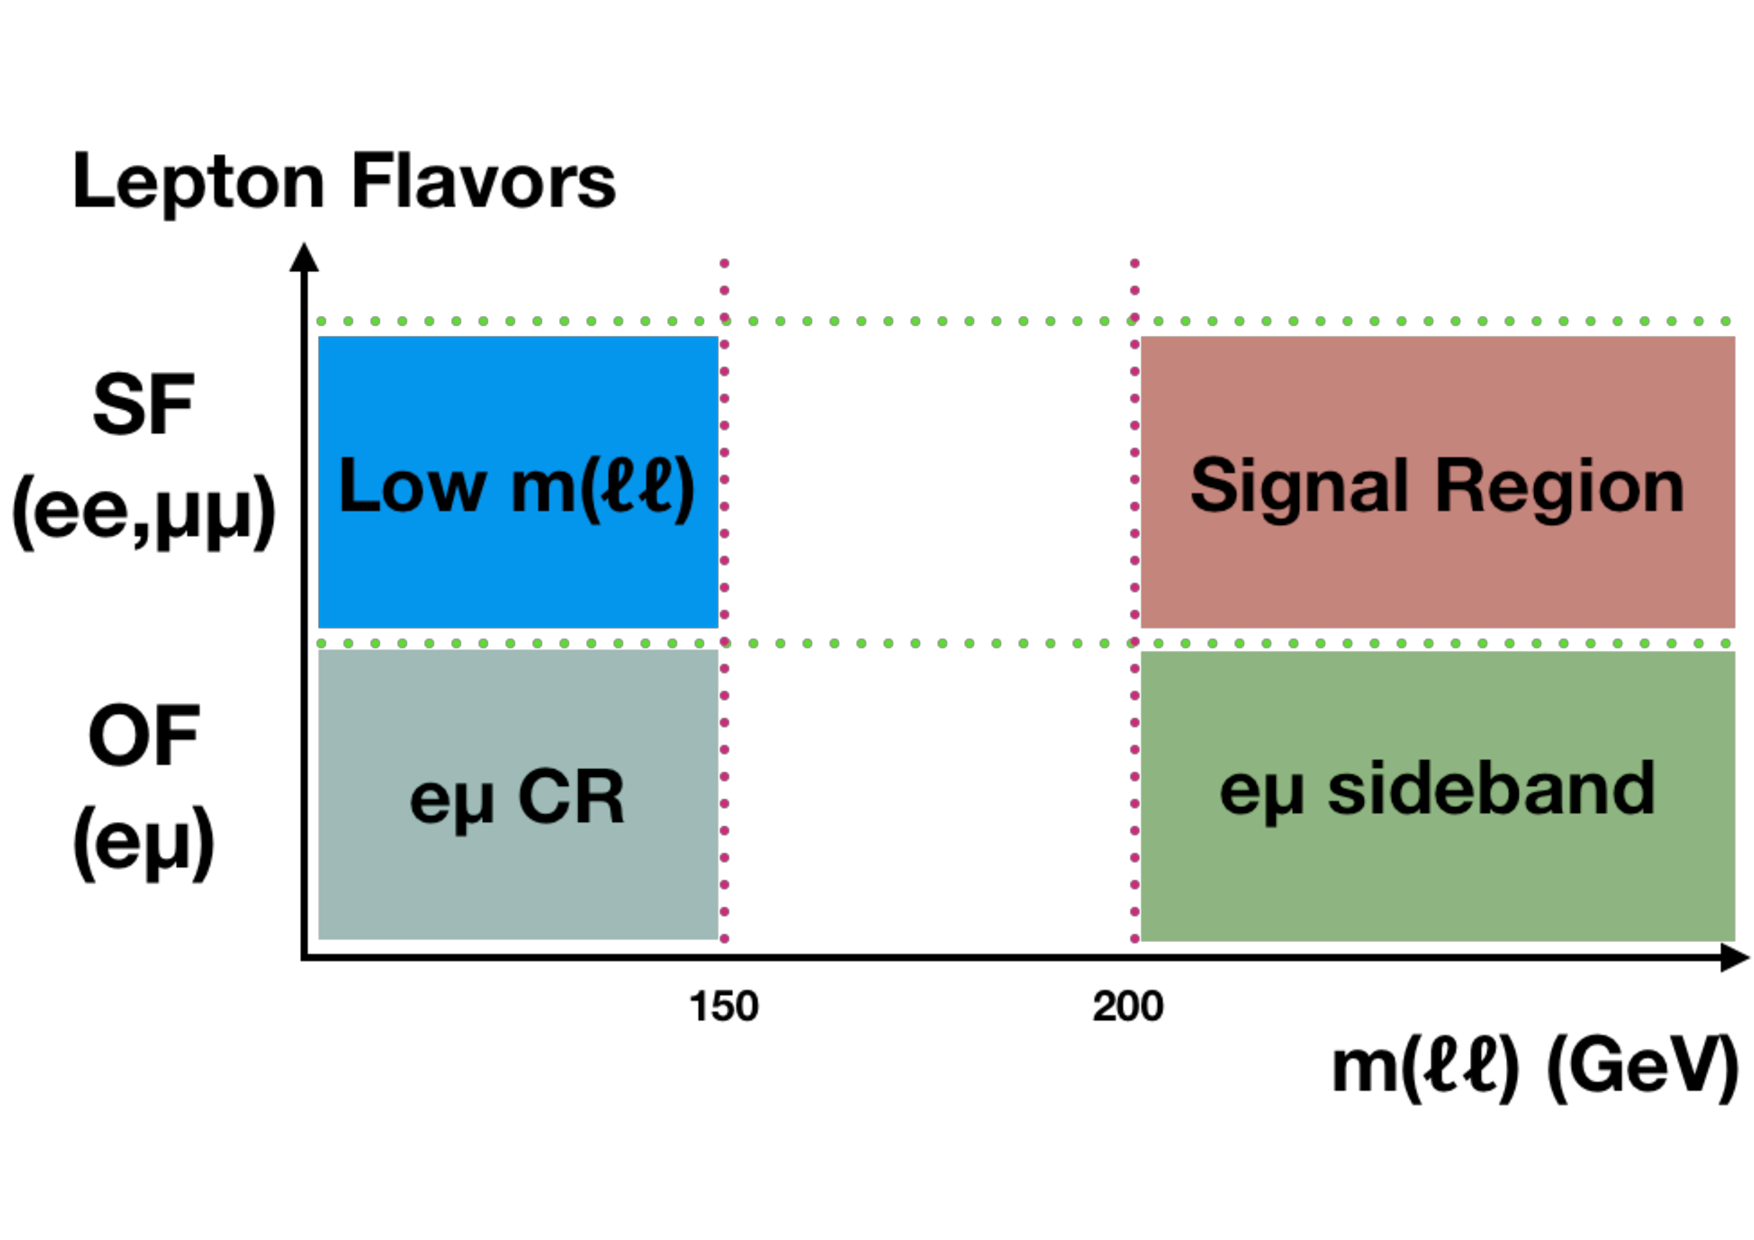
\includegraphics[width=1.0\textwidth]{figures/Schem.pdf}
  \topcaption{
    A schematic diagram of the analysis regions.
  }
  \label{fig:BkgdSchem}
\end{figure}

\subsection{Z+Jets background estimation}
MC simulation was used to estimate the background from high mass DY lepton pairs produced in association with additional jets.
The DY contribution normalization in simulation was then corrected to match the events in data by means of a SF measured in the low $m_{\ell\ell}$ CR.
The contribution from other backgrounds in this CR is taken from simulation and subtracted from the data to produce a pure DY sample.
This SF takes into account residual mis-modeling between data and simulation including the signal region requirements on the jets.

We calculated preliminary normalization SFs in a region similar to our low $m_{\ell\ell}$ control region, to test our procedure. The region used is defined by:

\begin{itemize}
  \item Exactly two same-flavor leptons, without additional tight lepton
  \item \pt of the leading (subleading) lepton $>60(53)\GeV$
  \item The invariant mass of the dilepton, $\abs{m(\ell\ell) - m(\PZ)} < 10\GeV$, where $m(\PZ)=91.1876\GeV$
\end{itemize}

The dilepton mass distribution in this region is shown in Fig~\ref{fig:BkgdZmllBefore}, and the obtained normalization scale factors are shown in Tab.~\ref{tab:BkgdZNormSF}.


\begin{figure}[htbp]
  \centering

  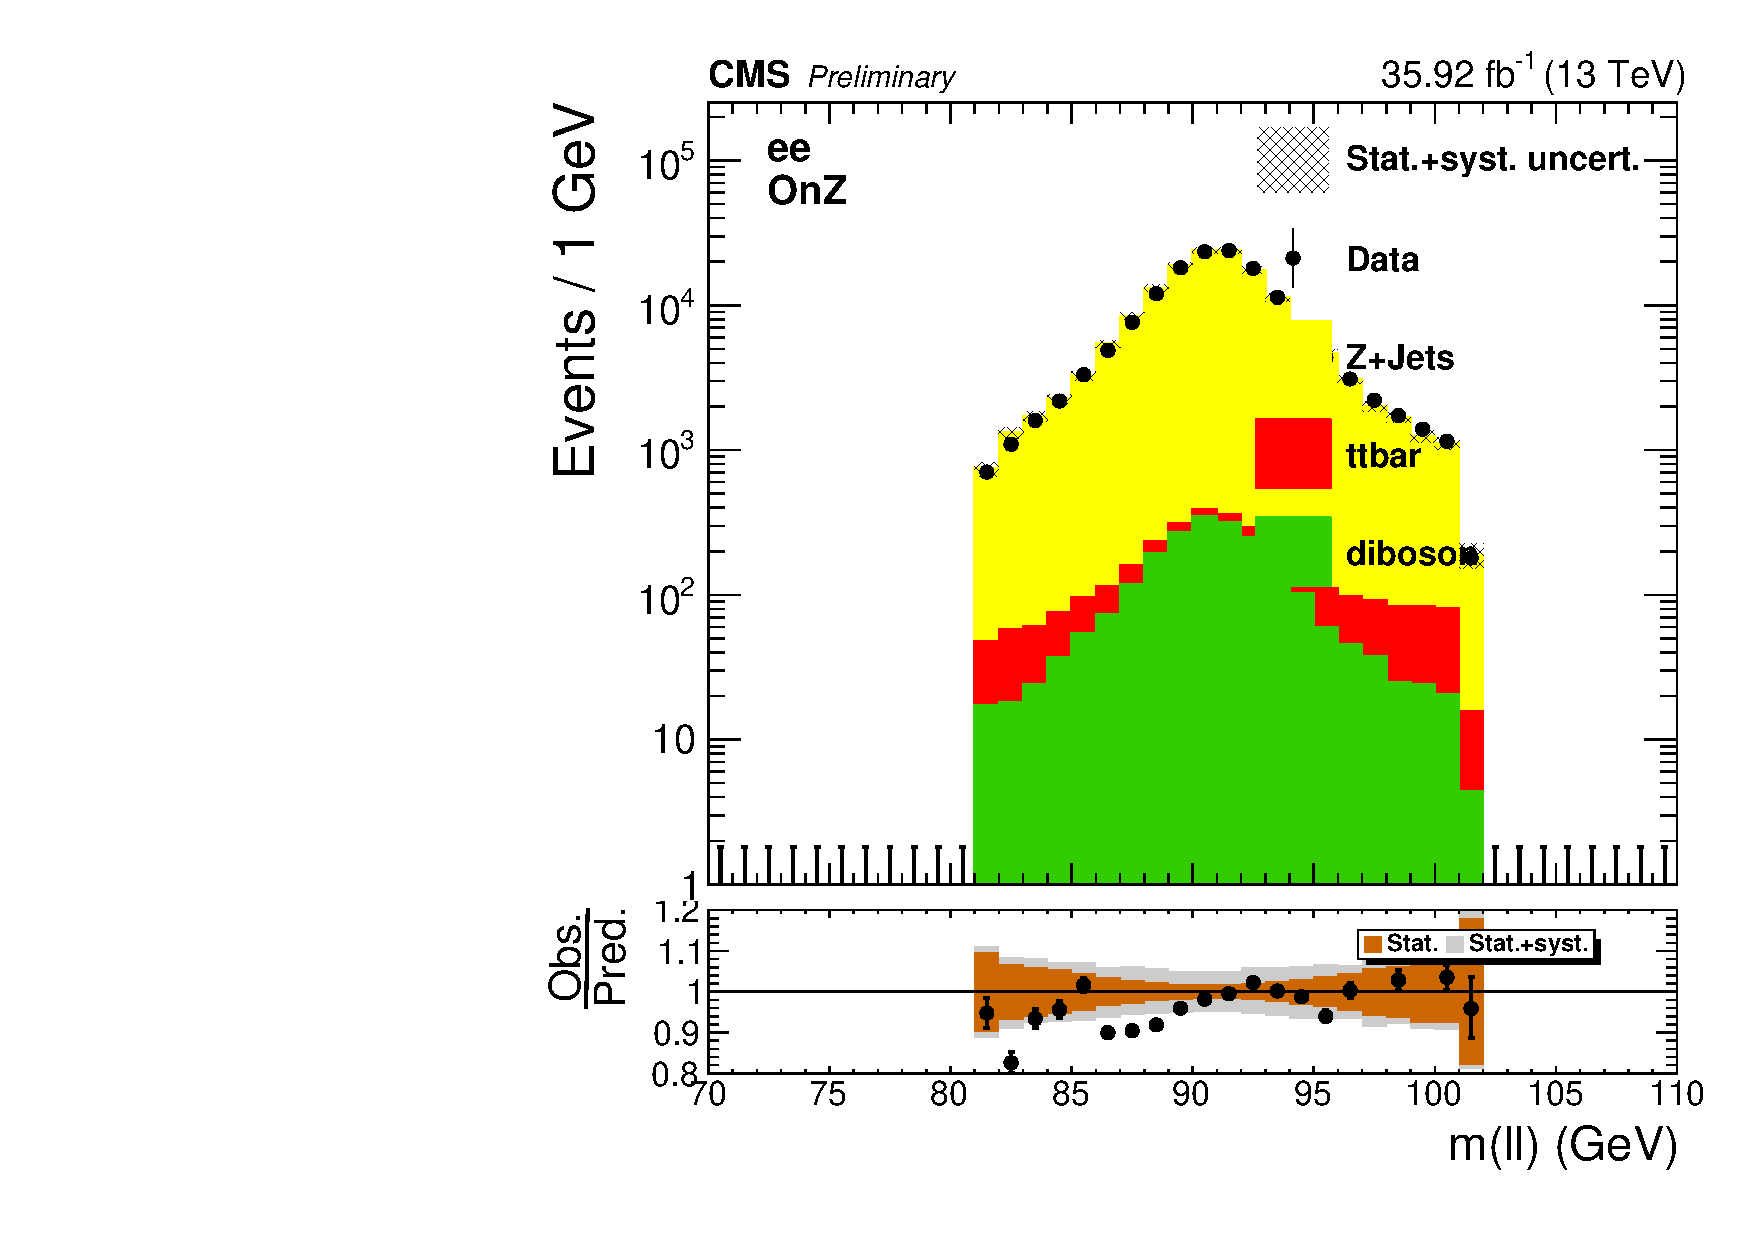
\includegraphics[width=0.45\textwidth]{figures/2016/BeforeNormSF_ZCand_Mass_HNWR_SingleElectron_OnZ.pdf}
  \hspace{0.01\textwidth}
  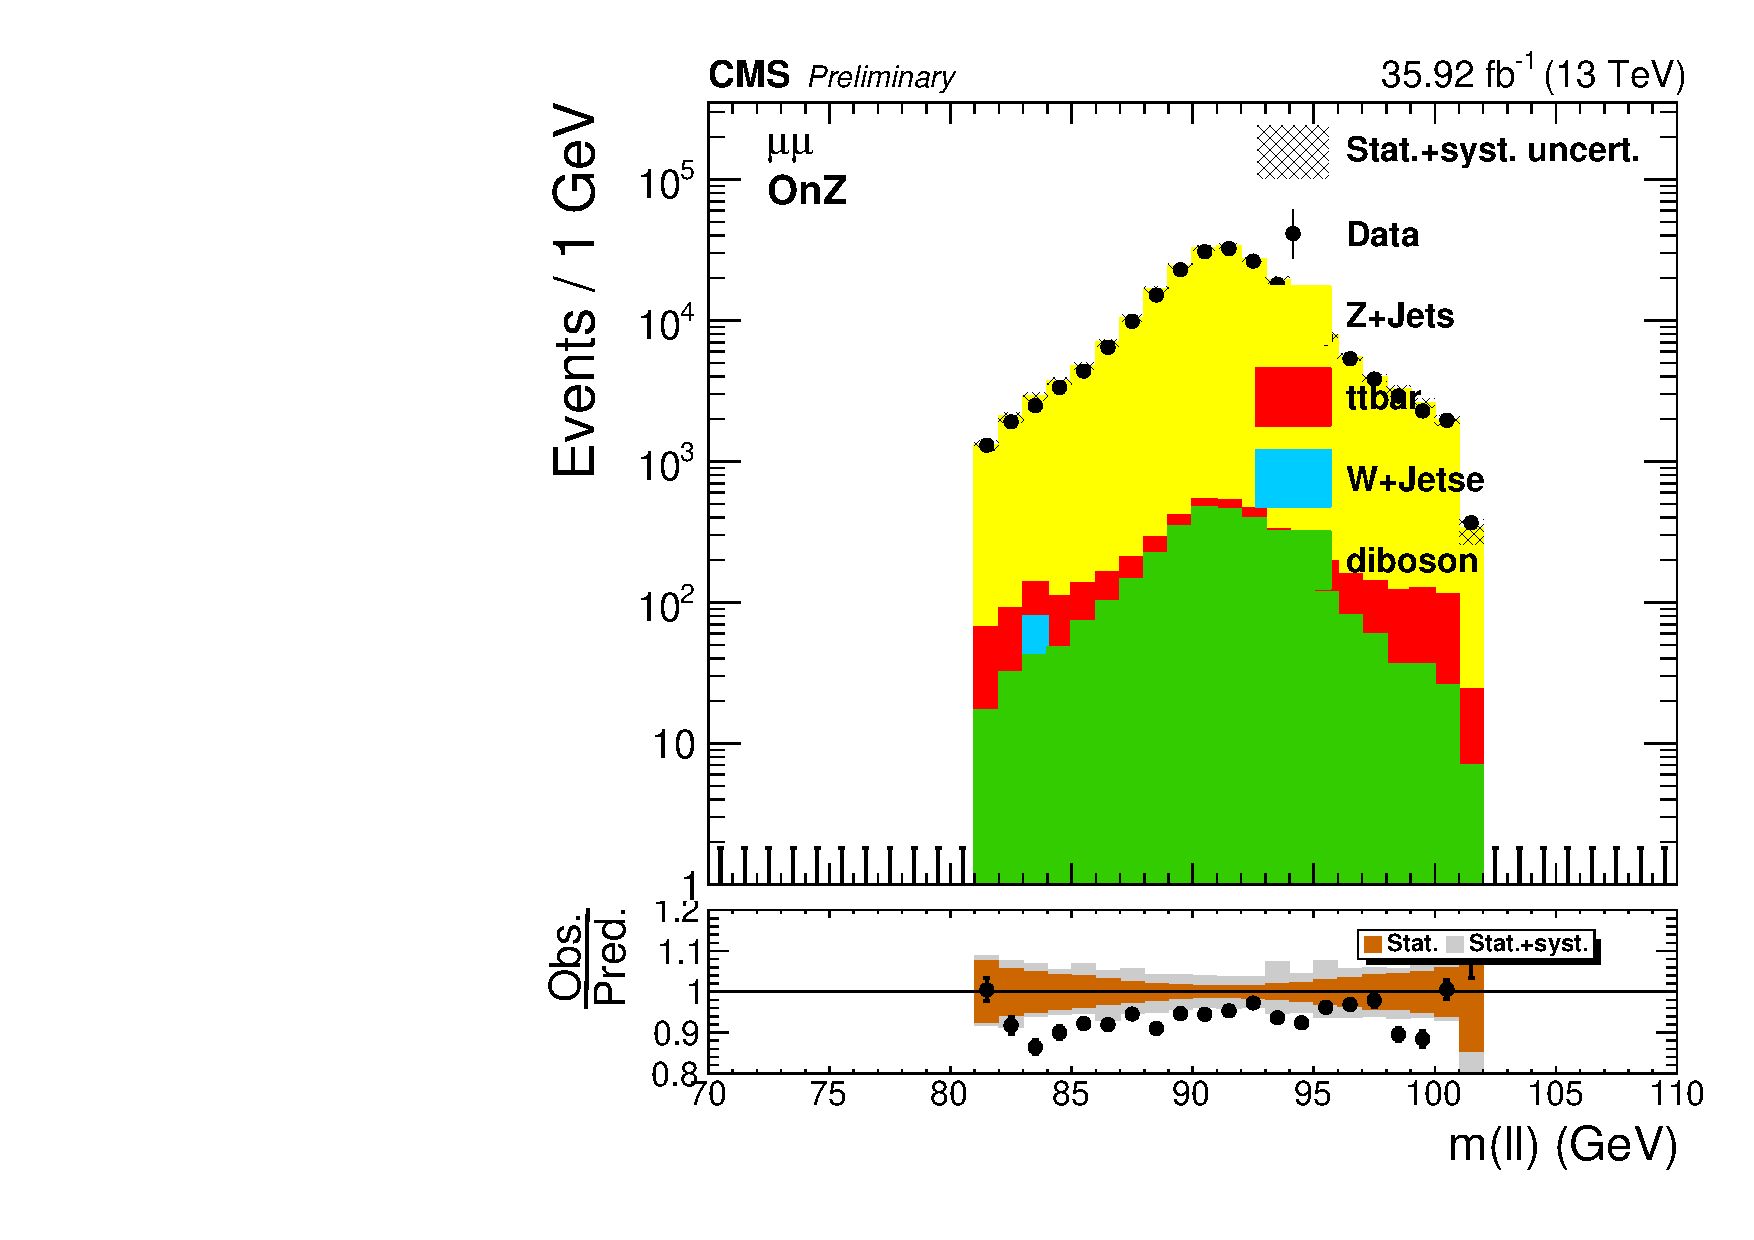
\includegraphics[width=0.45\textwidth]{figures/2016/BeforeNormSF_ZCand_Mass_HNWR_SingleMuon_OnZ.pdf}
  \vspace{0.01\textwidth}

  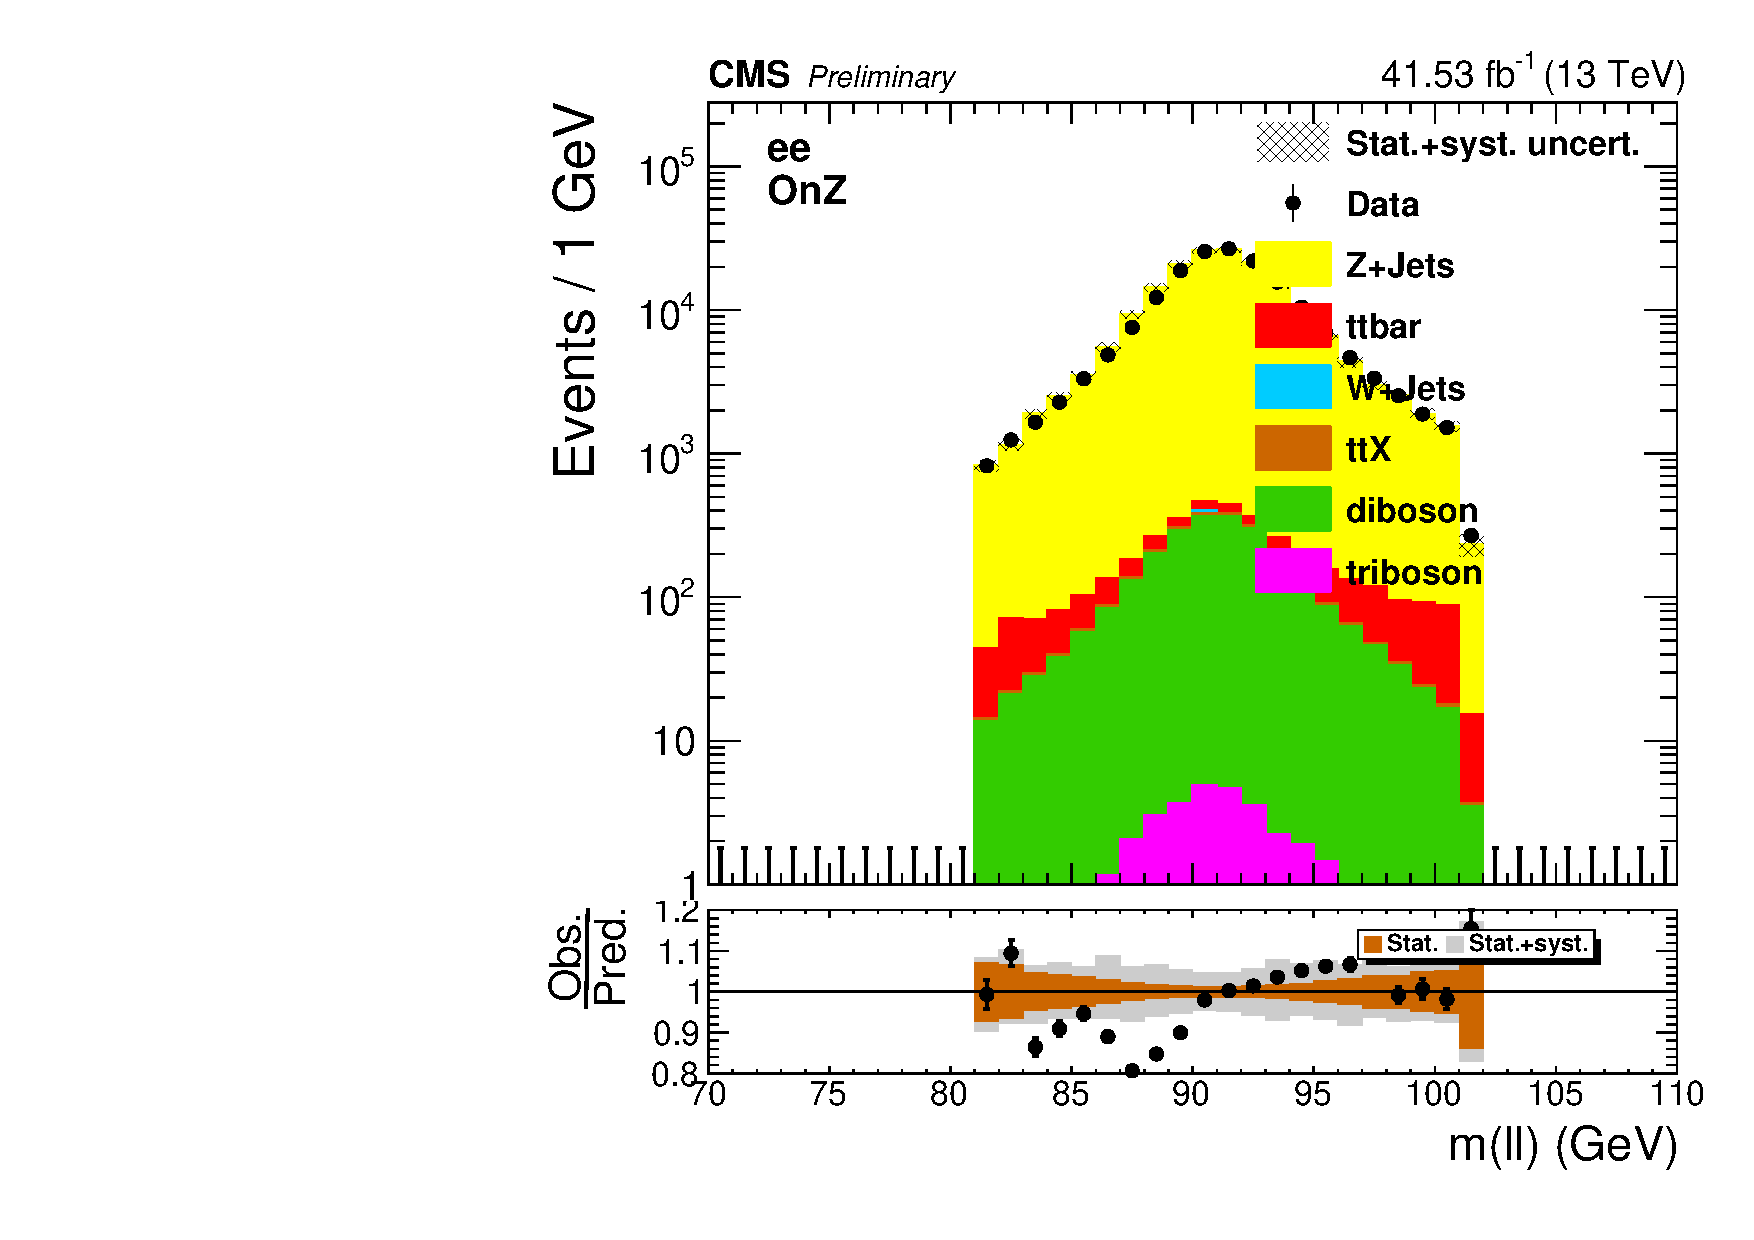
\includegraphics[width=0.45\textwidth]{figures/2017/BeforeNormSF_ZCand_Mass_HNWR_SingleElectron_OnZ.pdf}
  \hspace{0.01\textwidth}
  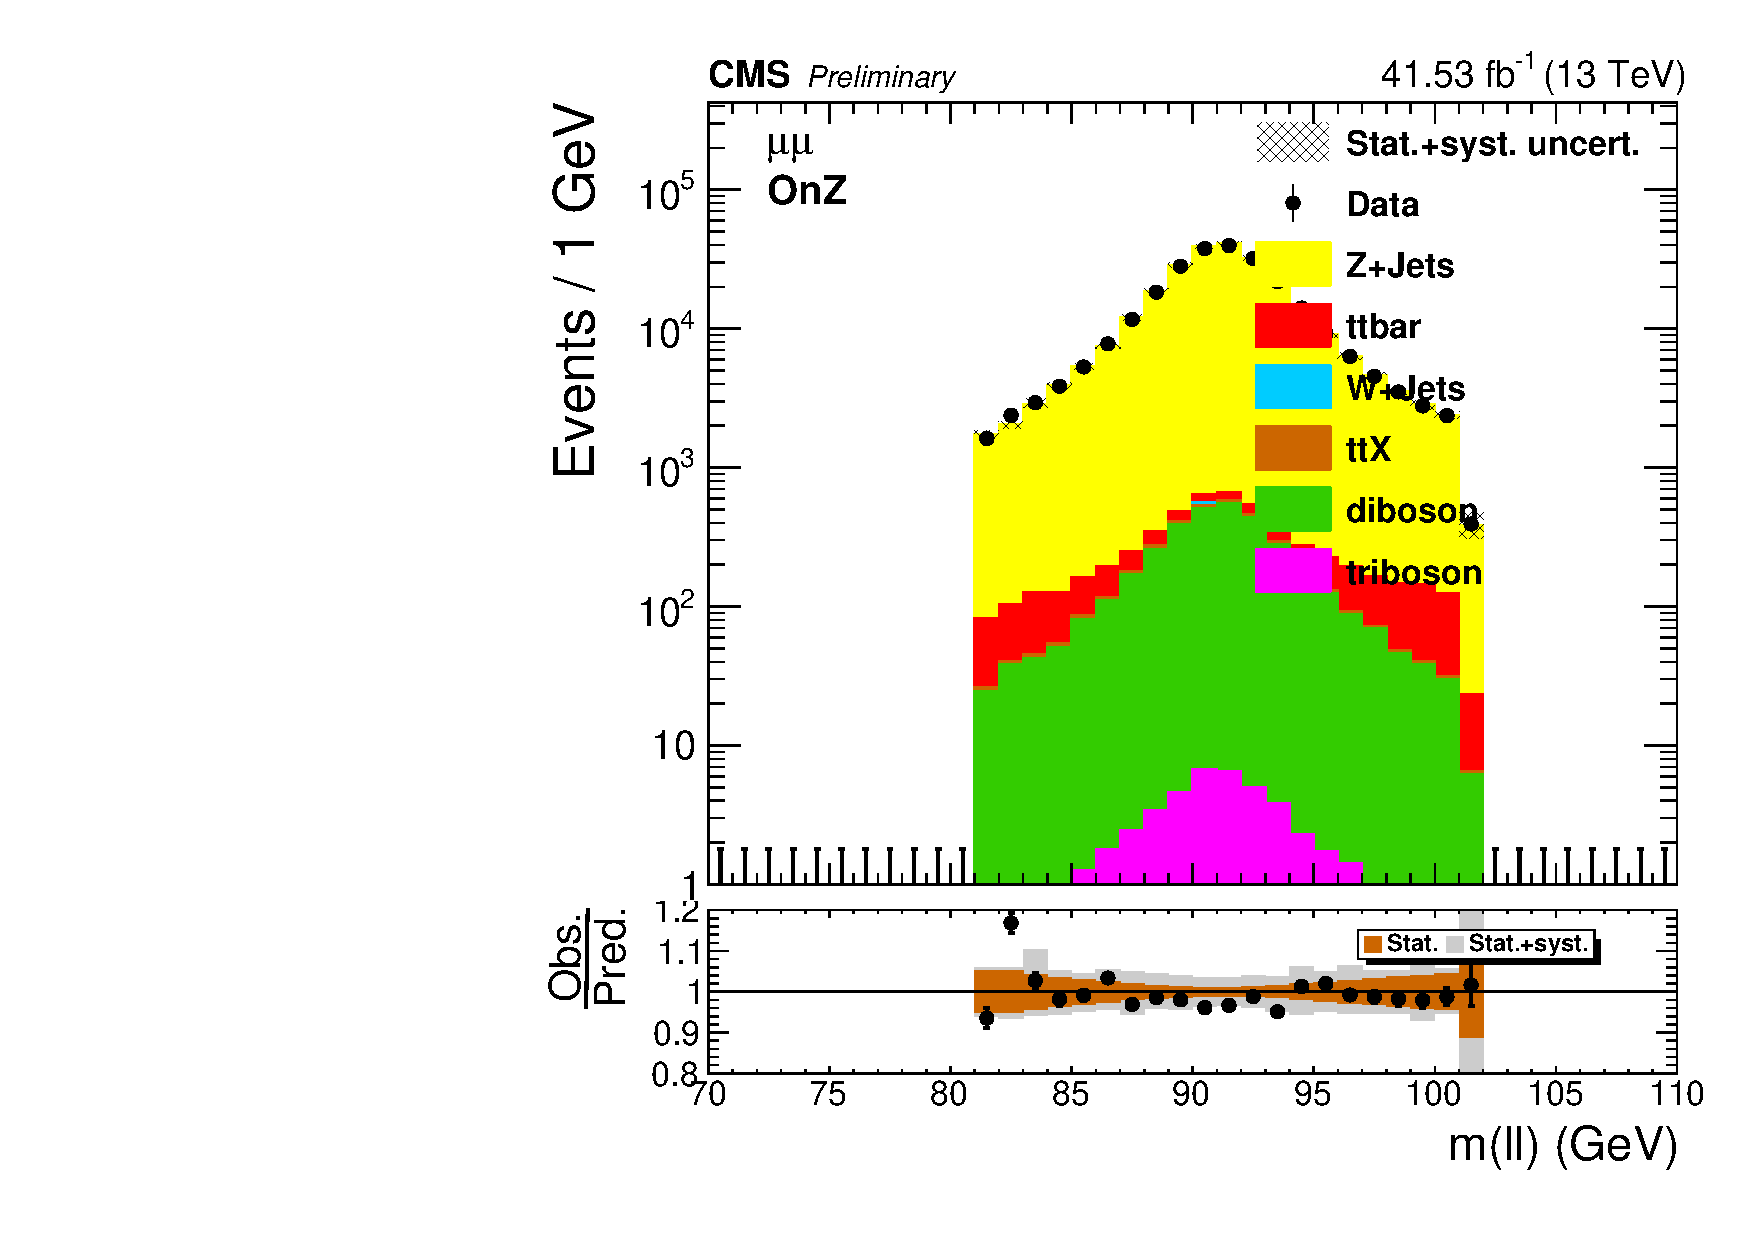
\includegraphics[width=0.45\textwidth]{figures/2017/BeforeNormSF_ZCand_Mass_HNWR_SingleMuon_OnZ.pdf}
  \vspace{0.01\textwidth}

  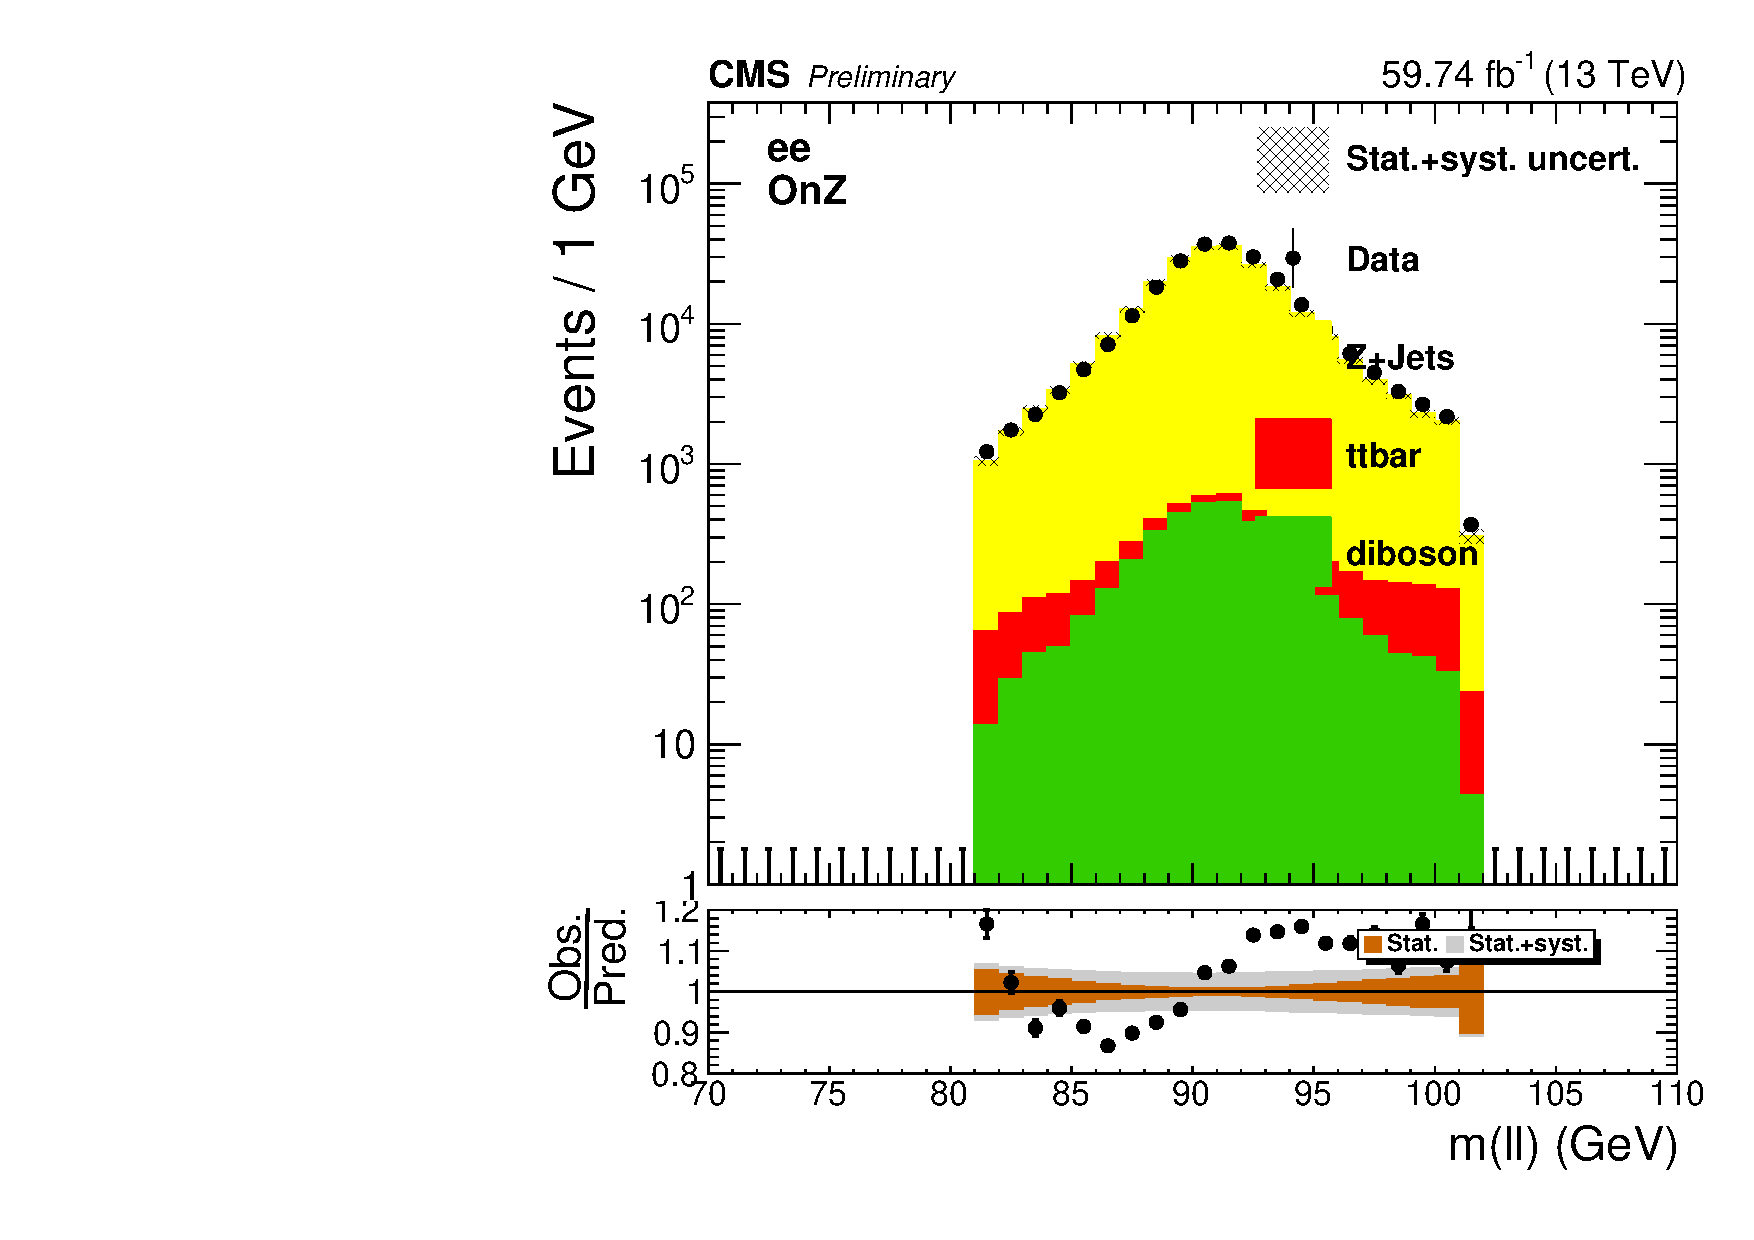
\includegraphics[width=0.45\textwidth]{figures/2018/BeforeNormSF_ZCand_Mass_HNWR_SingleElectron_OnZ.pdf}
  \hspace{0.01\textwidth}
  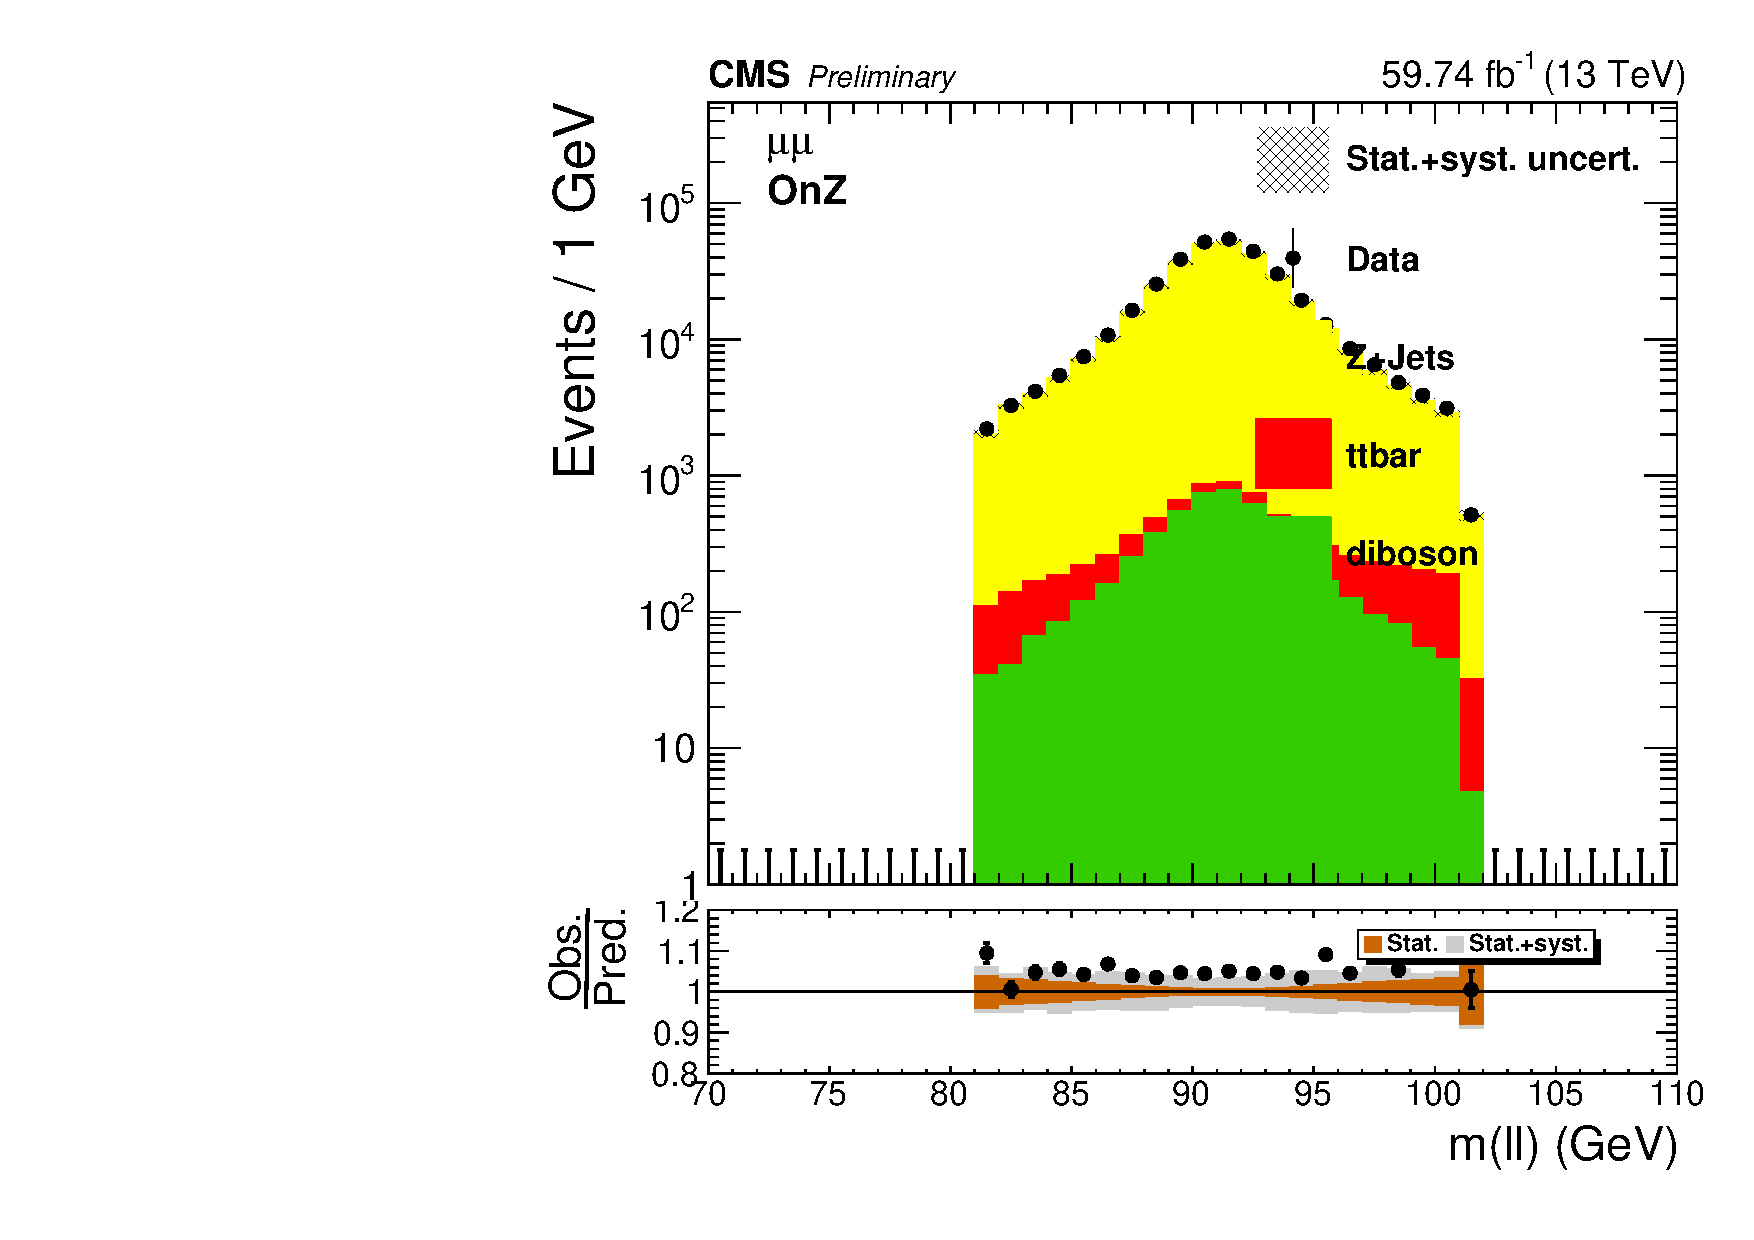
\includegraphics[width=0.45\textwidth]{figures/2018/BeforeNormSF_ZCand_Mass_HNWR_SingleMuon_OnZ.pdf}


  \topcaption{
    The dilepton mass distribution in the $\PZ$+Jets dominant control region, before applying the normalization scale factors.
    Results for dielectron (dimuon) channel is shown on the left (right), for 2016 (top), 2017 (middle) and 2018 (bottom).
  }
  \label{fig:BkgdZmllBefore}
\end{figure}

\begin{table}[htbp]
  \topcaption{
    The normalization scale factor of the $\PZ$+Jets MC samples.
  }
  \centering
  \label{tab:BkgdZNormSF}
  \begin{tabular}{ccc}
\hline
Year & $\Pe\Pe$ & $\mu\mu$ \\
\hline
2016 & $0.975 \pm 0.007\stat \pm 0.020\thy$ & $0.942 \pm 0.006\stat \pm 0.019\thy$ \\
2017 & $0.970 \pm 0.006\stat \pm 0.020\thy$ & $0.980 \pm 0.005\stat \pm 0.020\thy$ \\
2018 & $1.040 \pm 0.005\stat \pm 0.022\thy$ & $1.050 \pm 0.004\stat \pm 0.022\thy$ \\
\hline
  \end{tabular}
\end{table}


With this normalization scale factor applied, the dilepton \pt distribution is shown in Fig~\ref{fig:BkgdZptllAfter}.
Due to the poor agreement of the $\PZ$-\pt between the data and MC,
we reweighted the shape of the dilepton \pt distribution.
The reweighting function is shown in Fig.~\ref{fig:BkgdZptReweight}.
A constant value is used after 500~\GeV, using the value from the previous bin.
Figure~\ref{fig:BkgdZptLepPtBefore} and Figure~\ref{fig:BkgdZptLepPtAfter} shows the lepton \pt distributions before and after both corrections applied, respectively.

\begin{figure}[htbp]
  \centering

  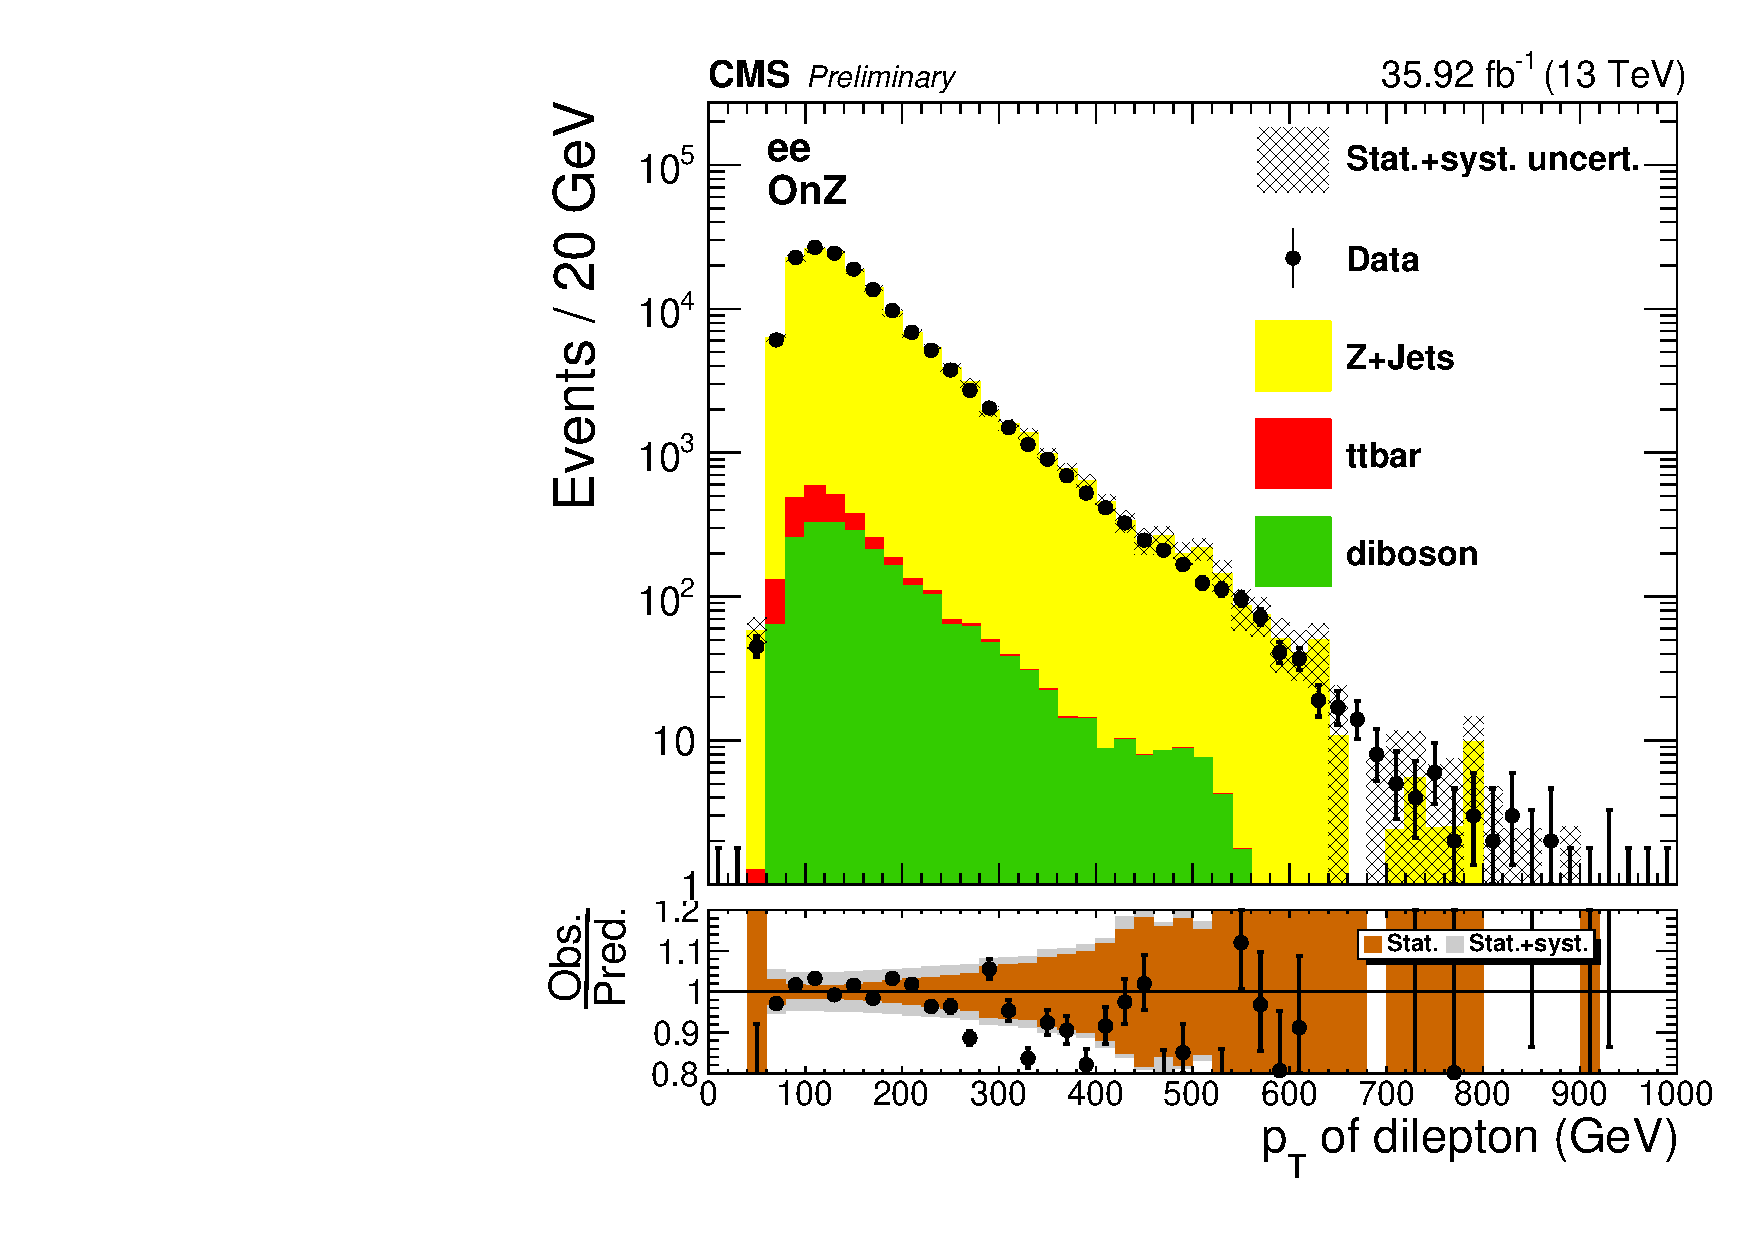
\includegraphics[width=0.45\textwidth]{figures/2016/AfterNormSF_ZCand_Pt_HNWR_SingleElectron_OnZ.pdf}
  \hspace{0.01\textwidth}
  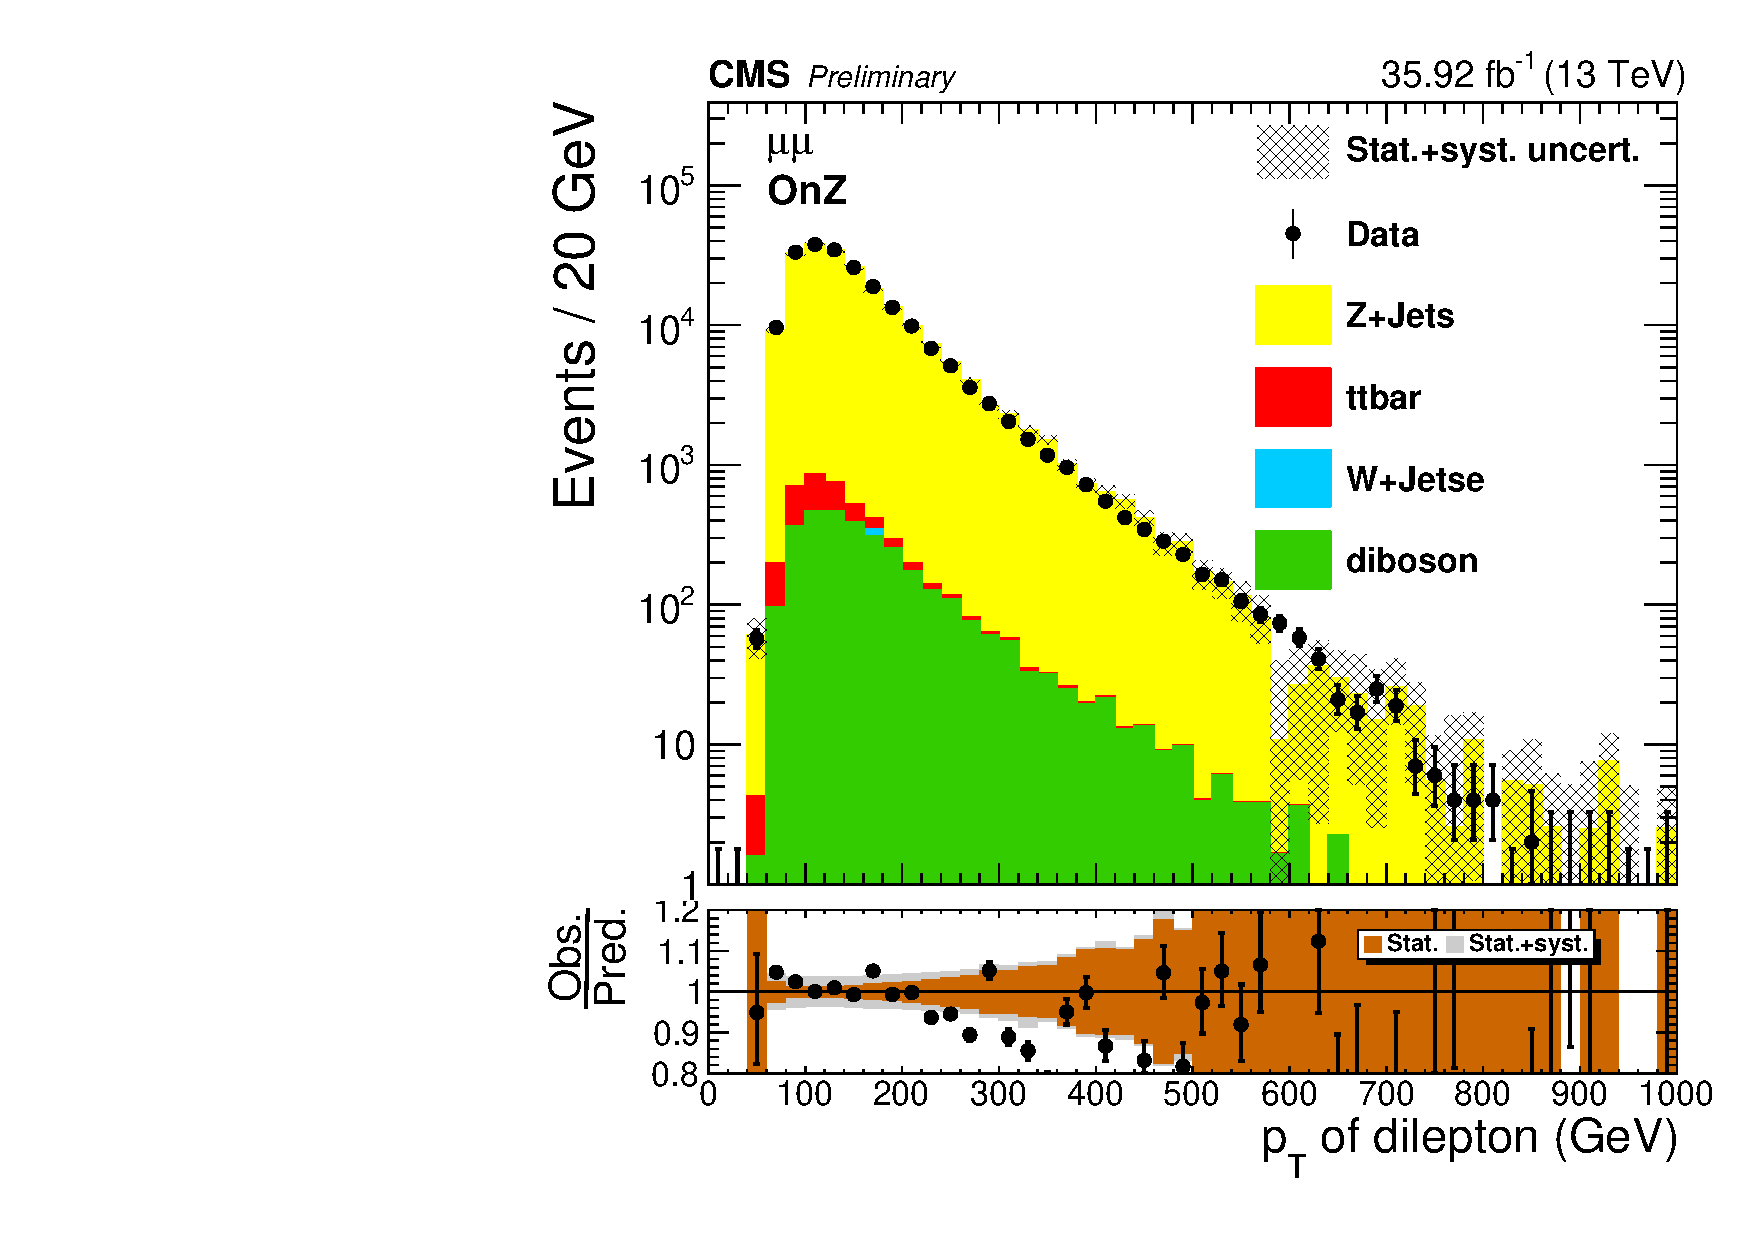
\includegraphics[width=0.45\textwidth]{figures/2016/AfterNormSF_ZCand_Pt_HNWR_SingleMuon_OnZ.pdf}
  \vspace{0.01\textwidth}

  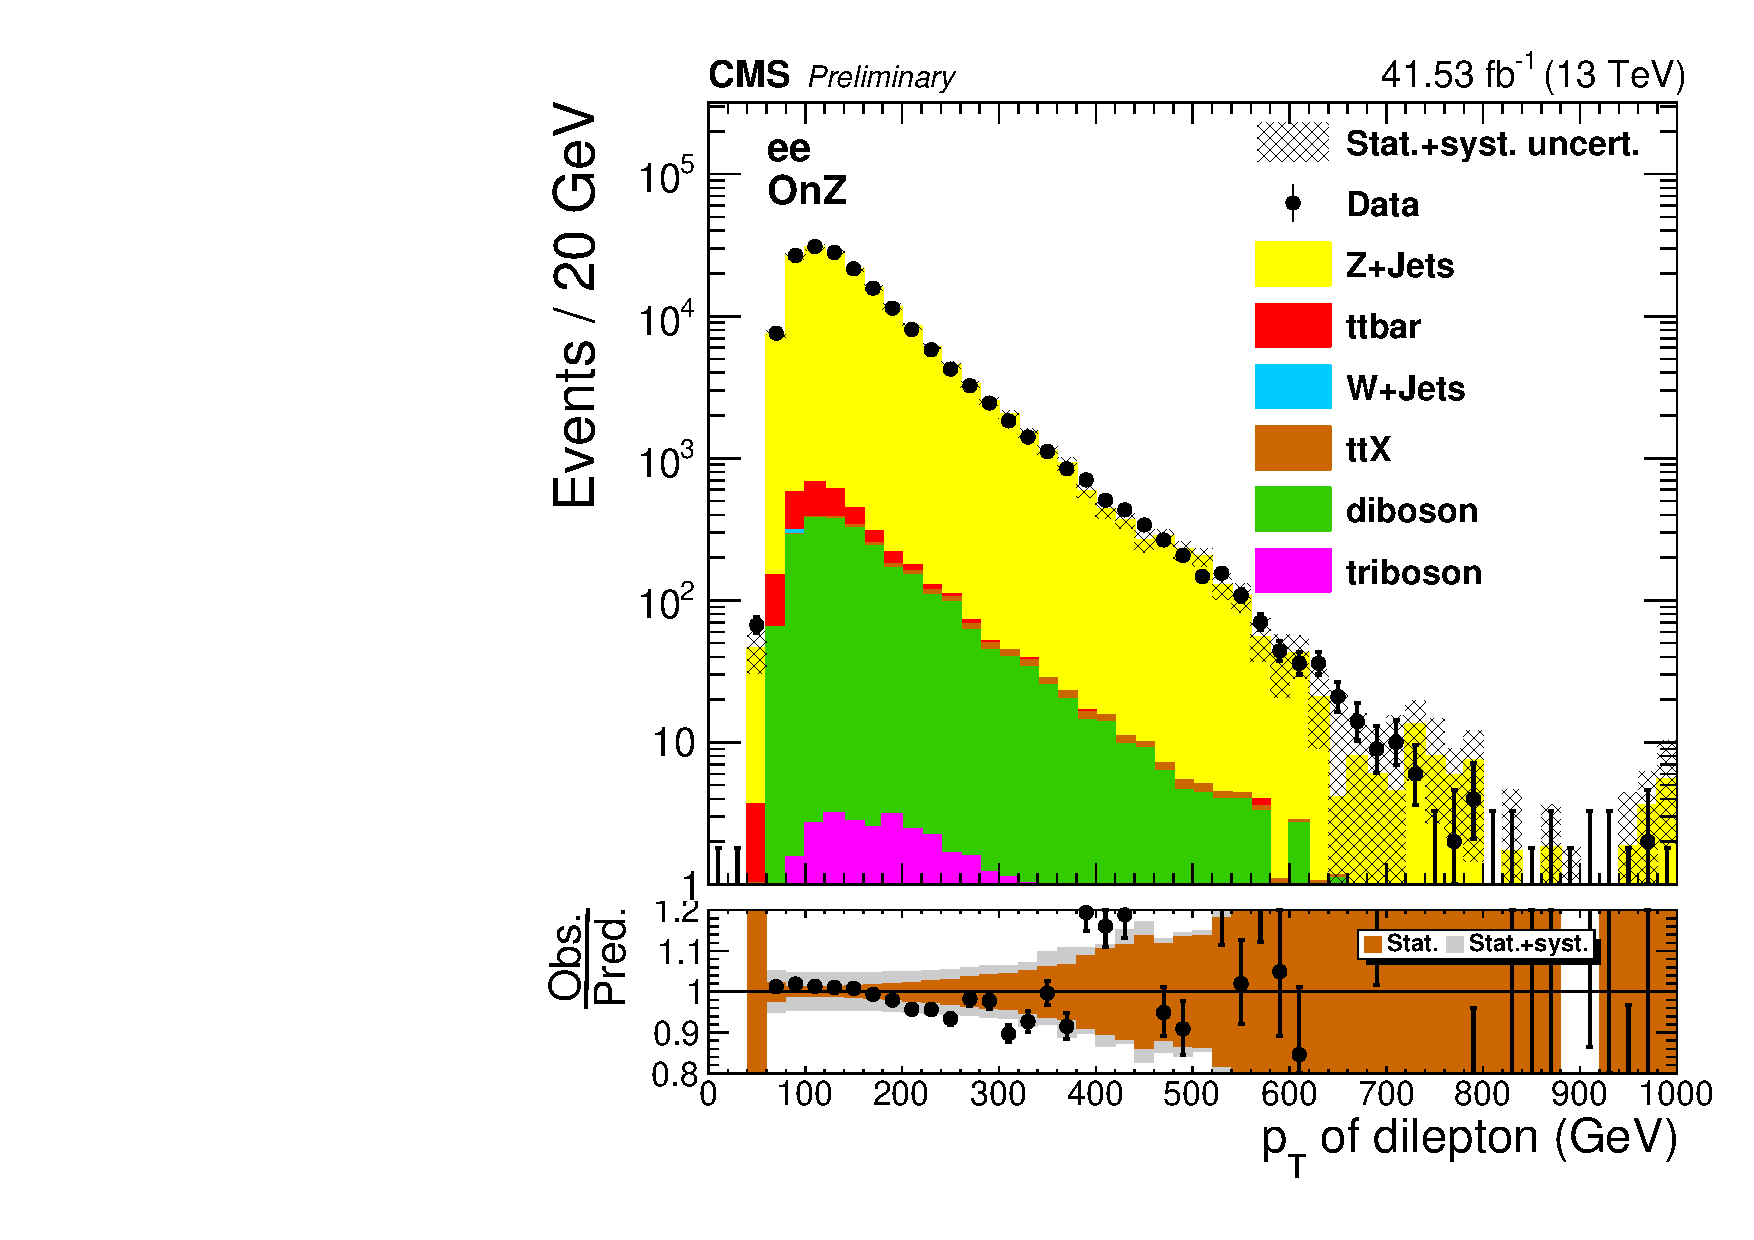
\includegraphics[width=0.45\textwidth]{figures/2017/AfterNormSF_ZCand_Pt_HNWR_SingleElectron_OnZ.pdf}
  \hspace{0.01\textwidth}
  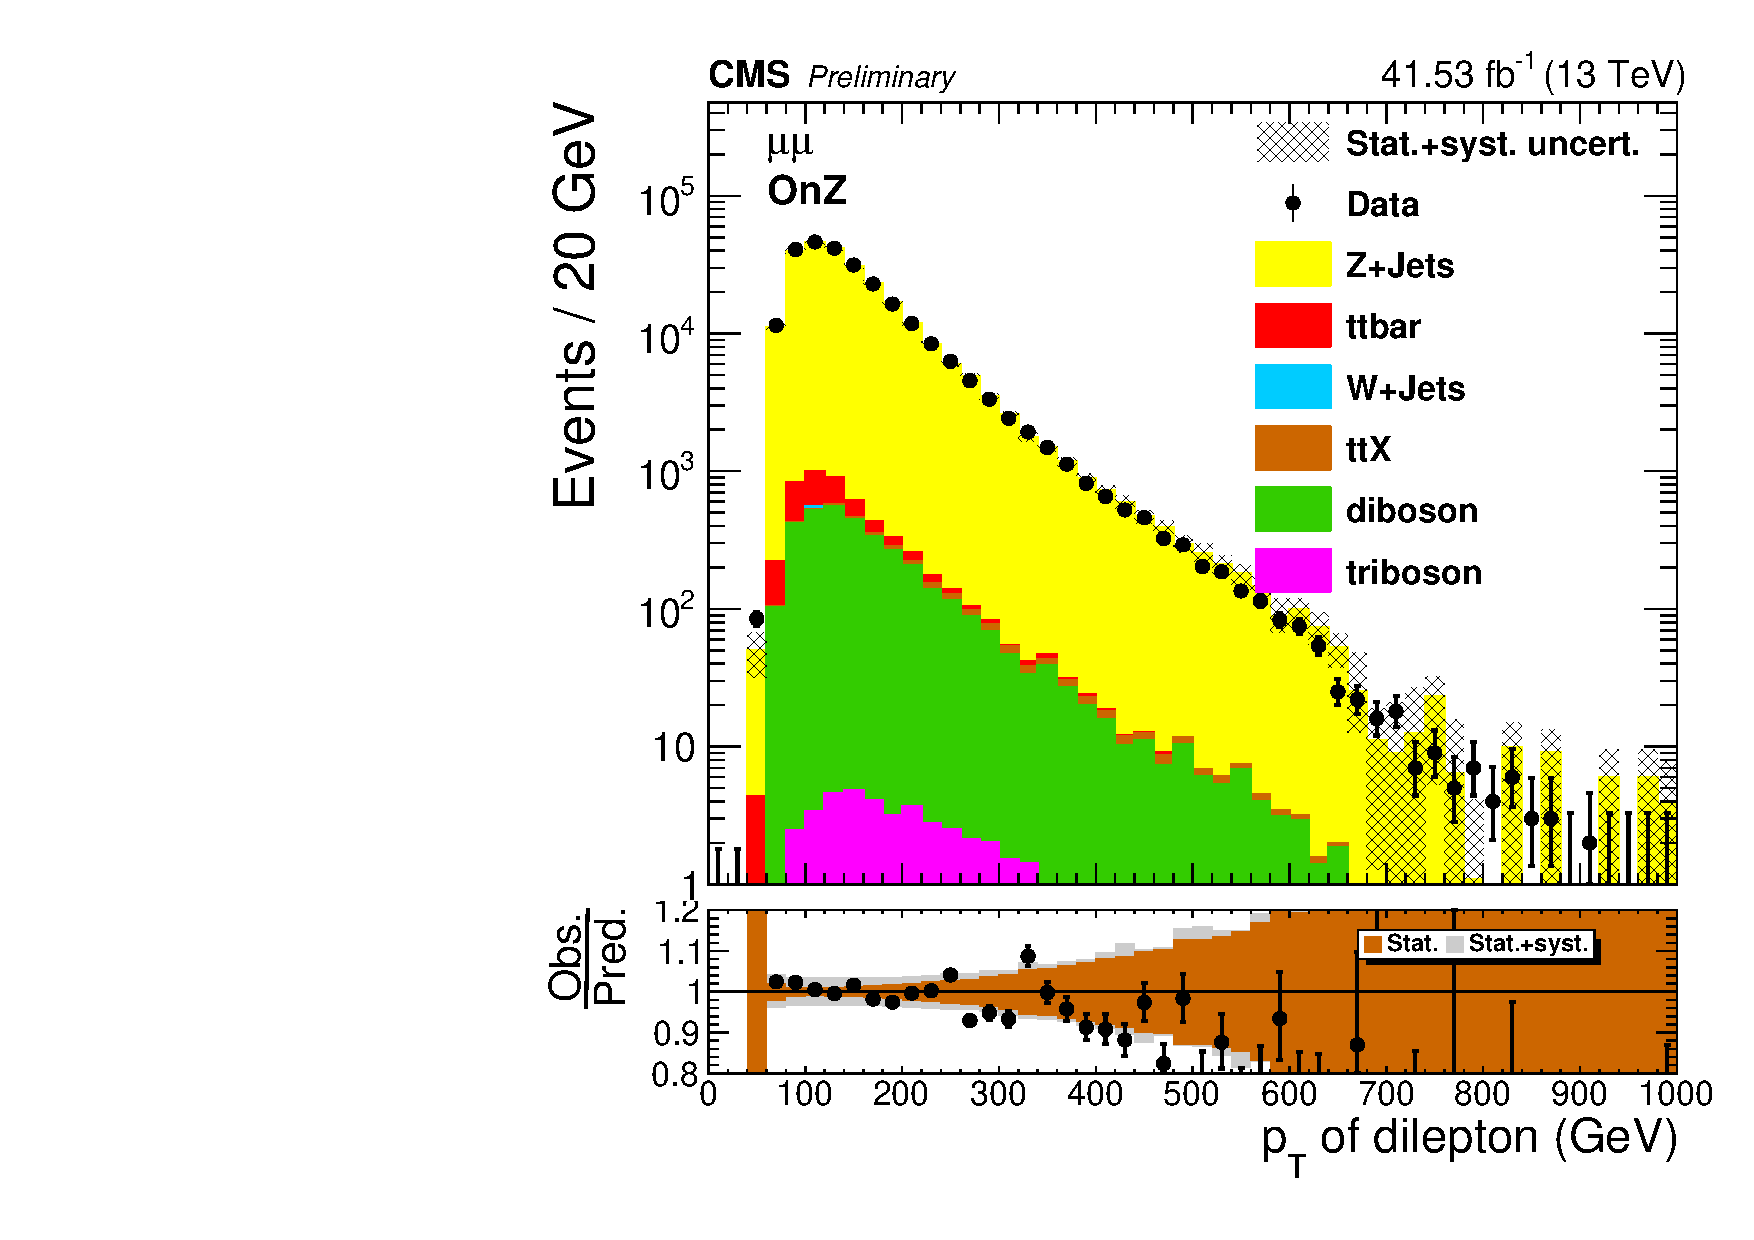
\includegraphics[width=0.45\textwidth]{figures/2017/AfterNormSF_ZCand_Pt_HNWR_SingleMuon_OnZ.pdf}
  \vspace{0.01\textwidth}
  
  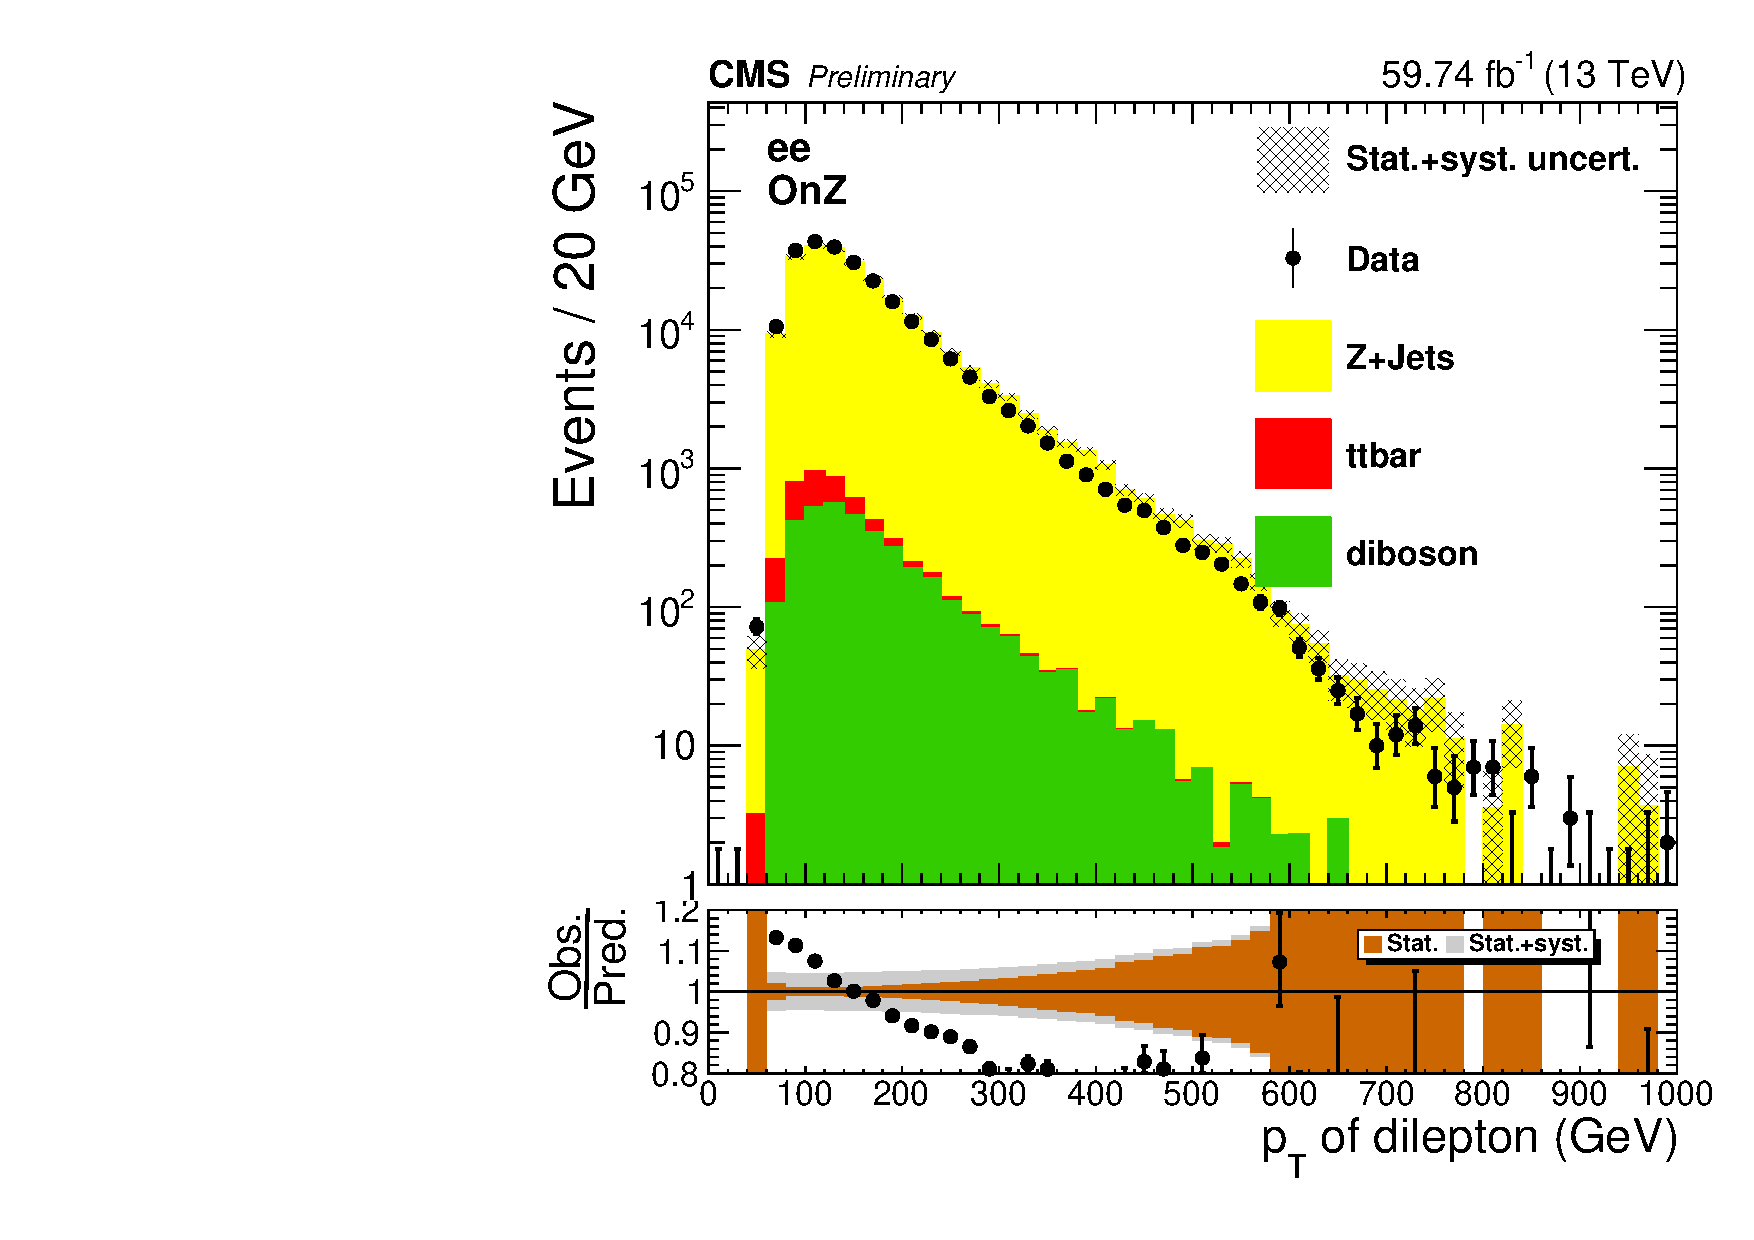
\includegraphics[width=0.45\textwidth]{figures/2018/AfterNormSF_ZCand_Pt_HNWR_SingleElectron_OnZ.pdf}
  \hspace{0.01\textwidth}
  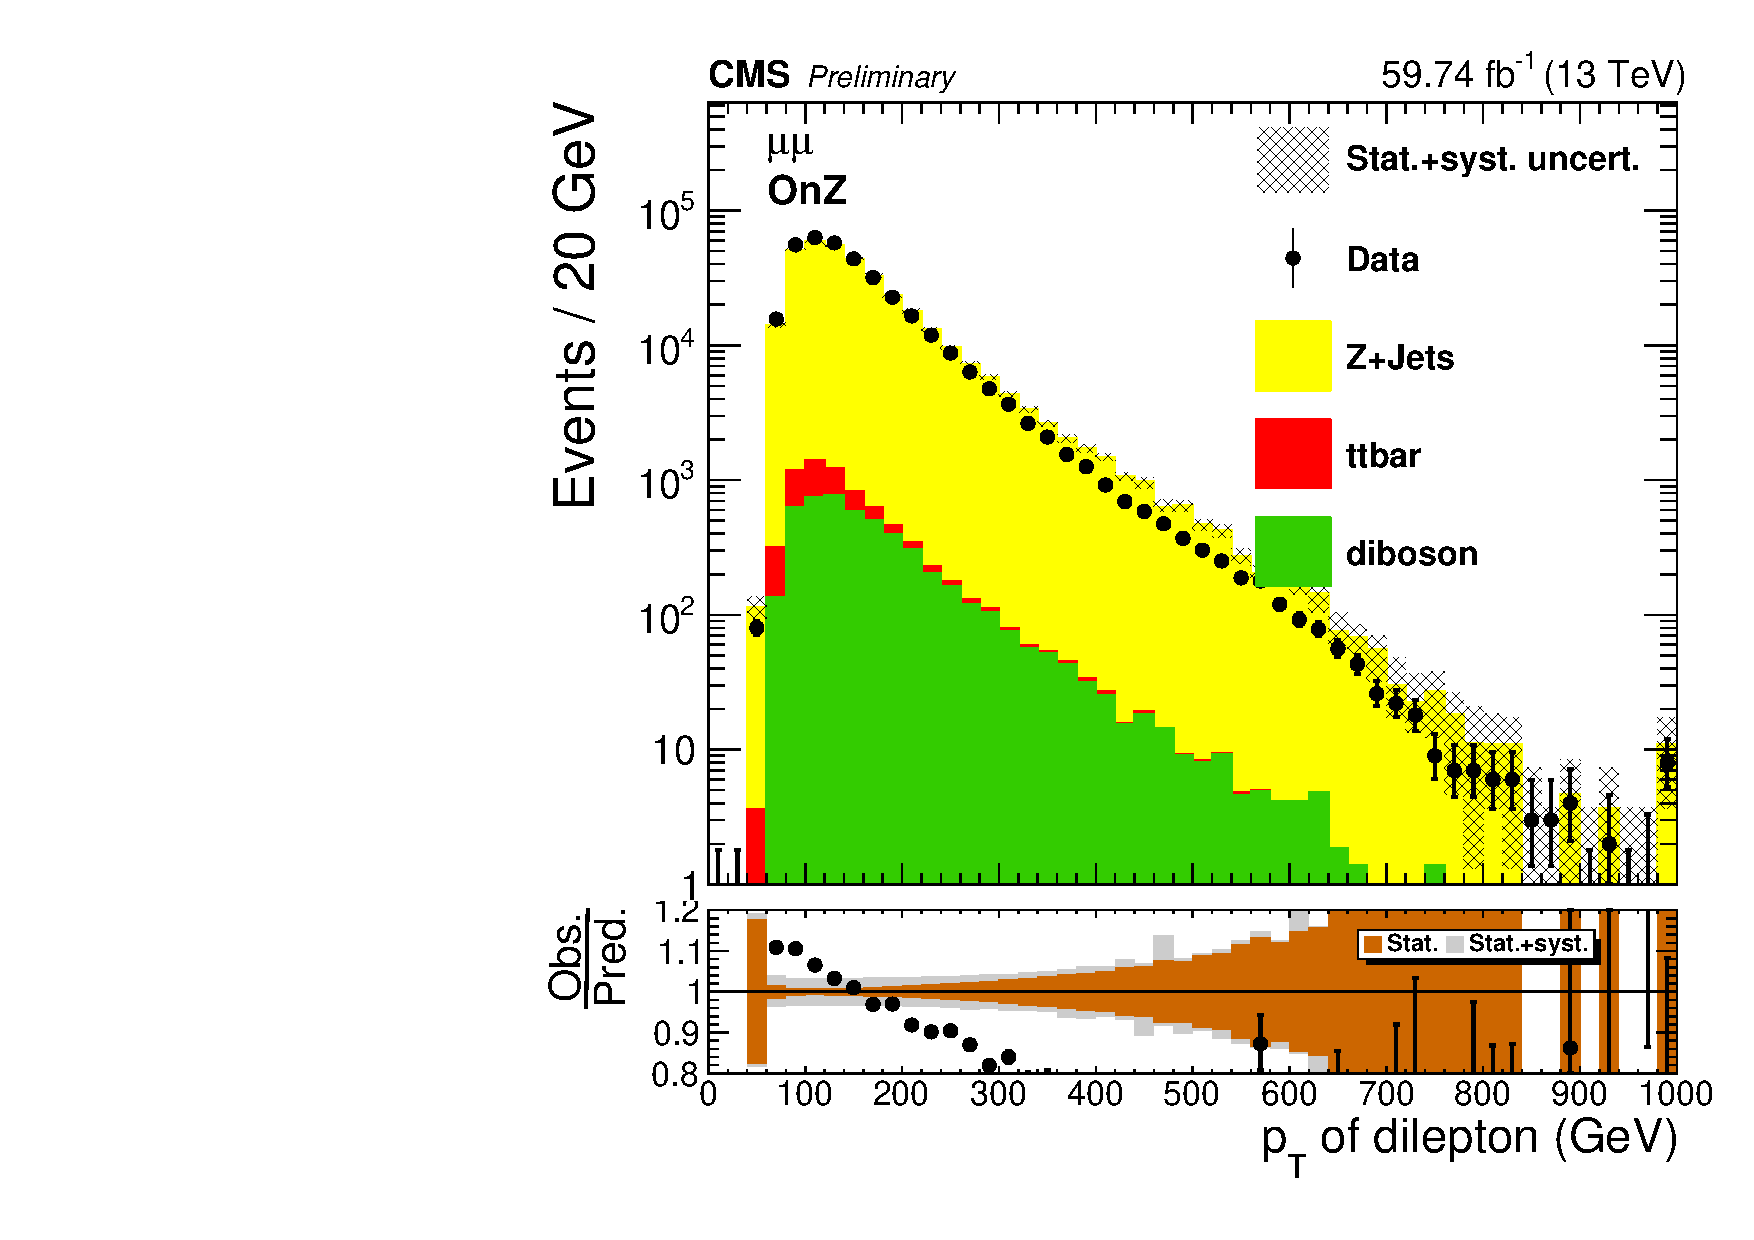
\includegraphics[width=0.45\textwidth]{figures/2018/AfterNormSF_ZCand_Pt_HNWR_SingleMuon_OnZ.pdf}

  \topcaption{
    The dilepton \pt distribution in the $\PZ$+Jets dominant control region, after applying the normalization scale factors.
    Results for dielectron (dimuon) channel is shown on the left (right), for 2016 (top), 2017 (middle) and 2018 (bottom).
  }
  \label{fig:BkgdZptllAfter}
\end{figure}

\begin{figure}[htbp]
  \centering

  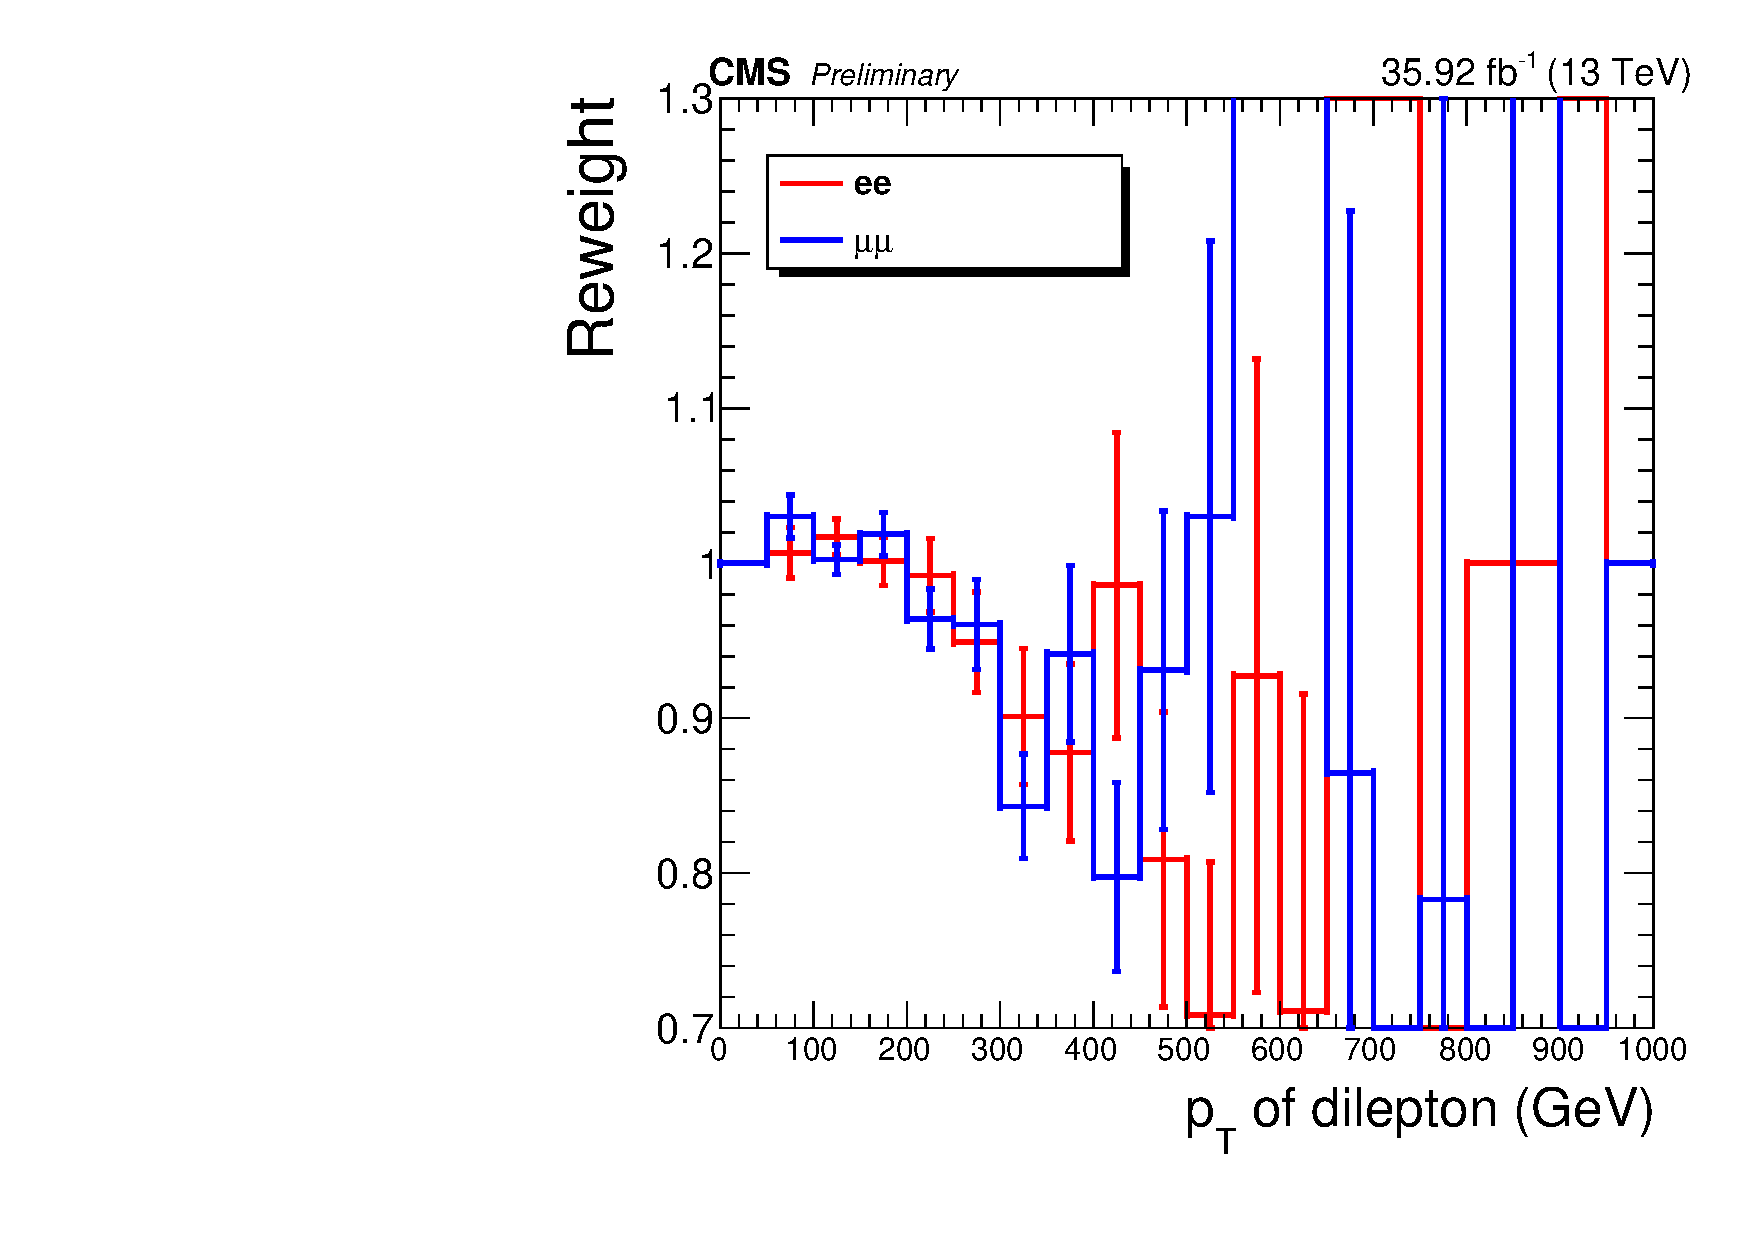
\includegraphics[width=0.45\textwidth]{figures/2016/Reweight.pdf}
  \hspace{0.01\textwidth}

  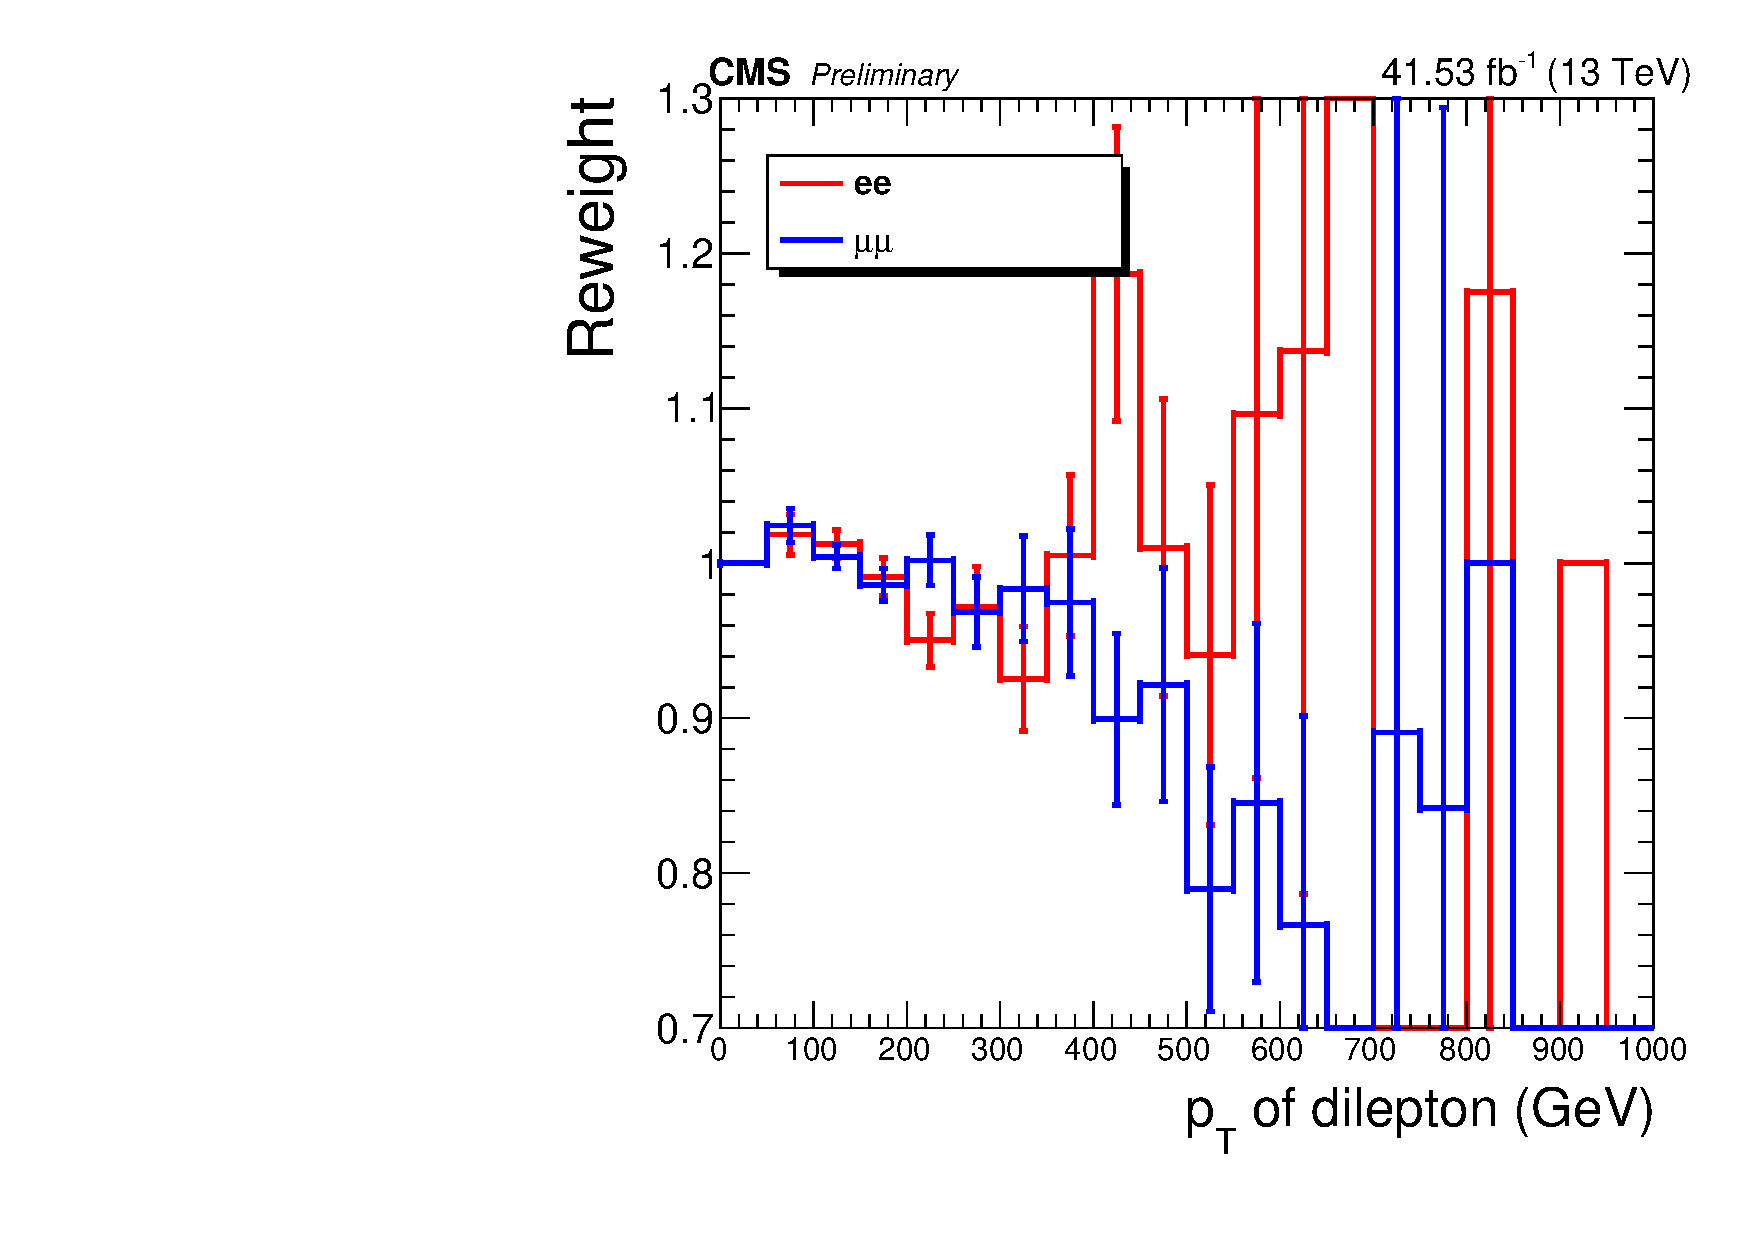
\includegraphics[width=0.45\textwidth]{figures/2017/Reweight.pdf}
  \hspace{0.01\textwidth}

  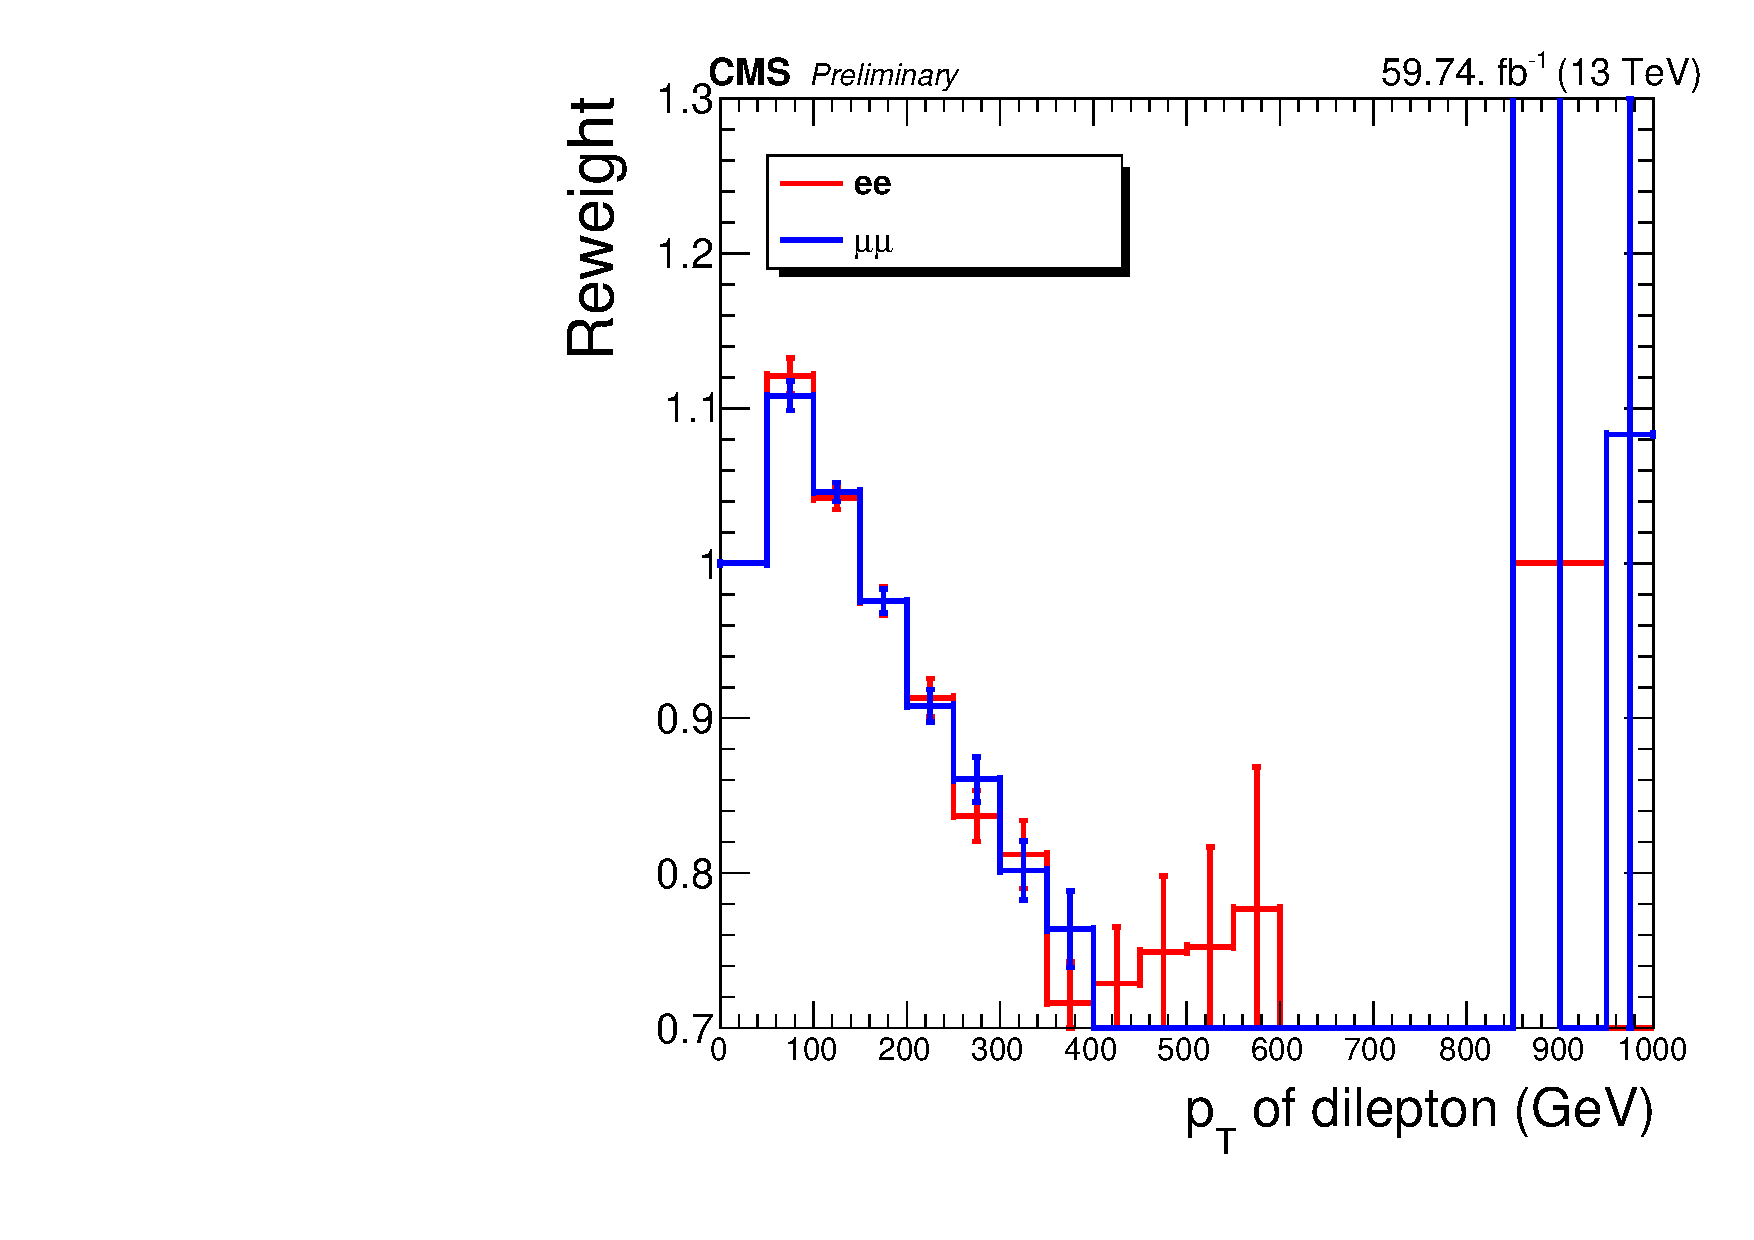
\includegraphics[width=0.45\textwidth]{figures/2018/Reweight.pdf}

  \topcaption{
    The dilepton \pt reweighting function, for 2016 (left), 2017 (middle) and 2018 (right).
  }
  \label{fig:BkgdZptReweight}
\end{figure}

\begin{figure}[htbp]
  \centering

  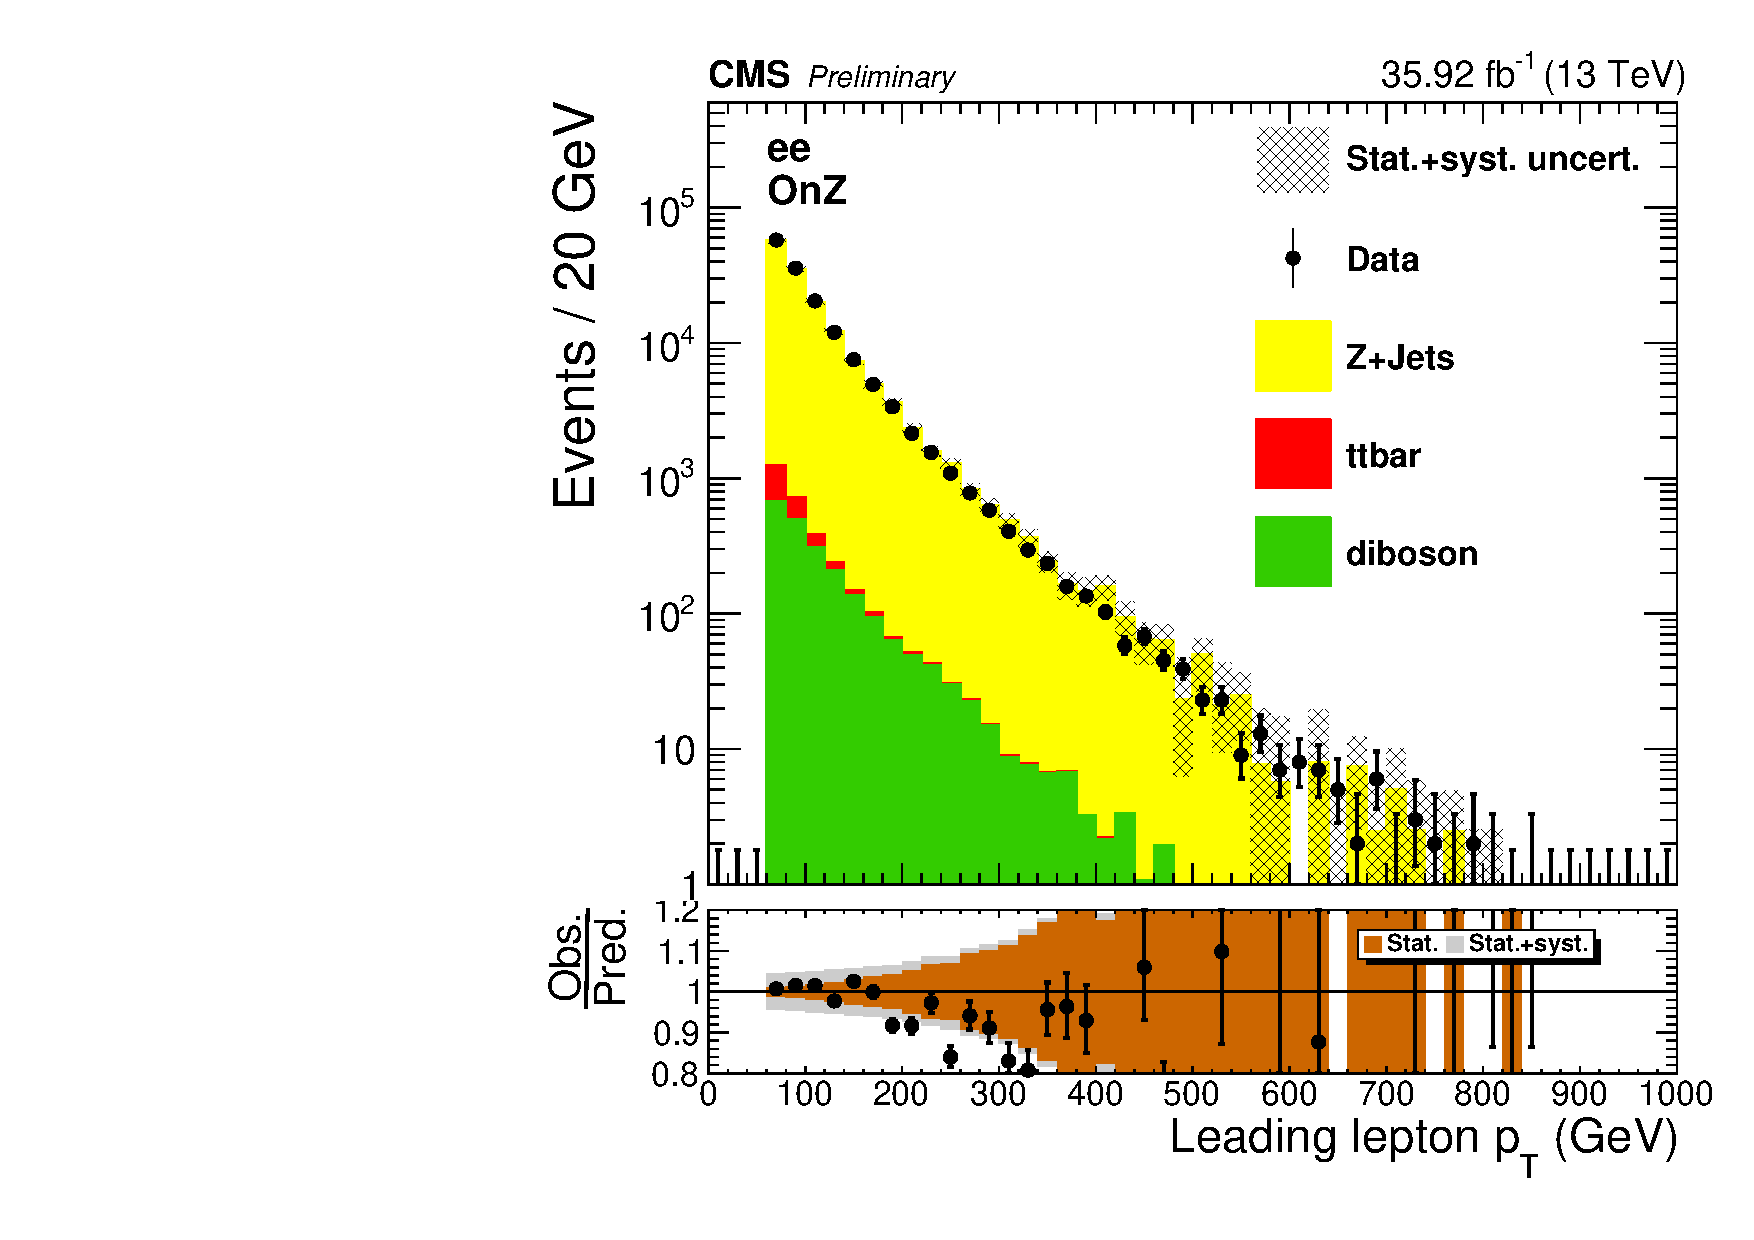
\includegraphics[width=0.45\textwidth]{figures/2016/AfterNormSF_Lepton_0_Pt_HNWR_SingleElectron_OnZ.pdf}
  \hspace{0.01\textwidth}
  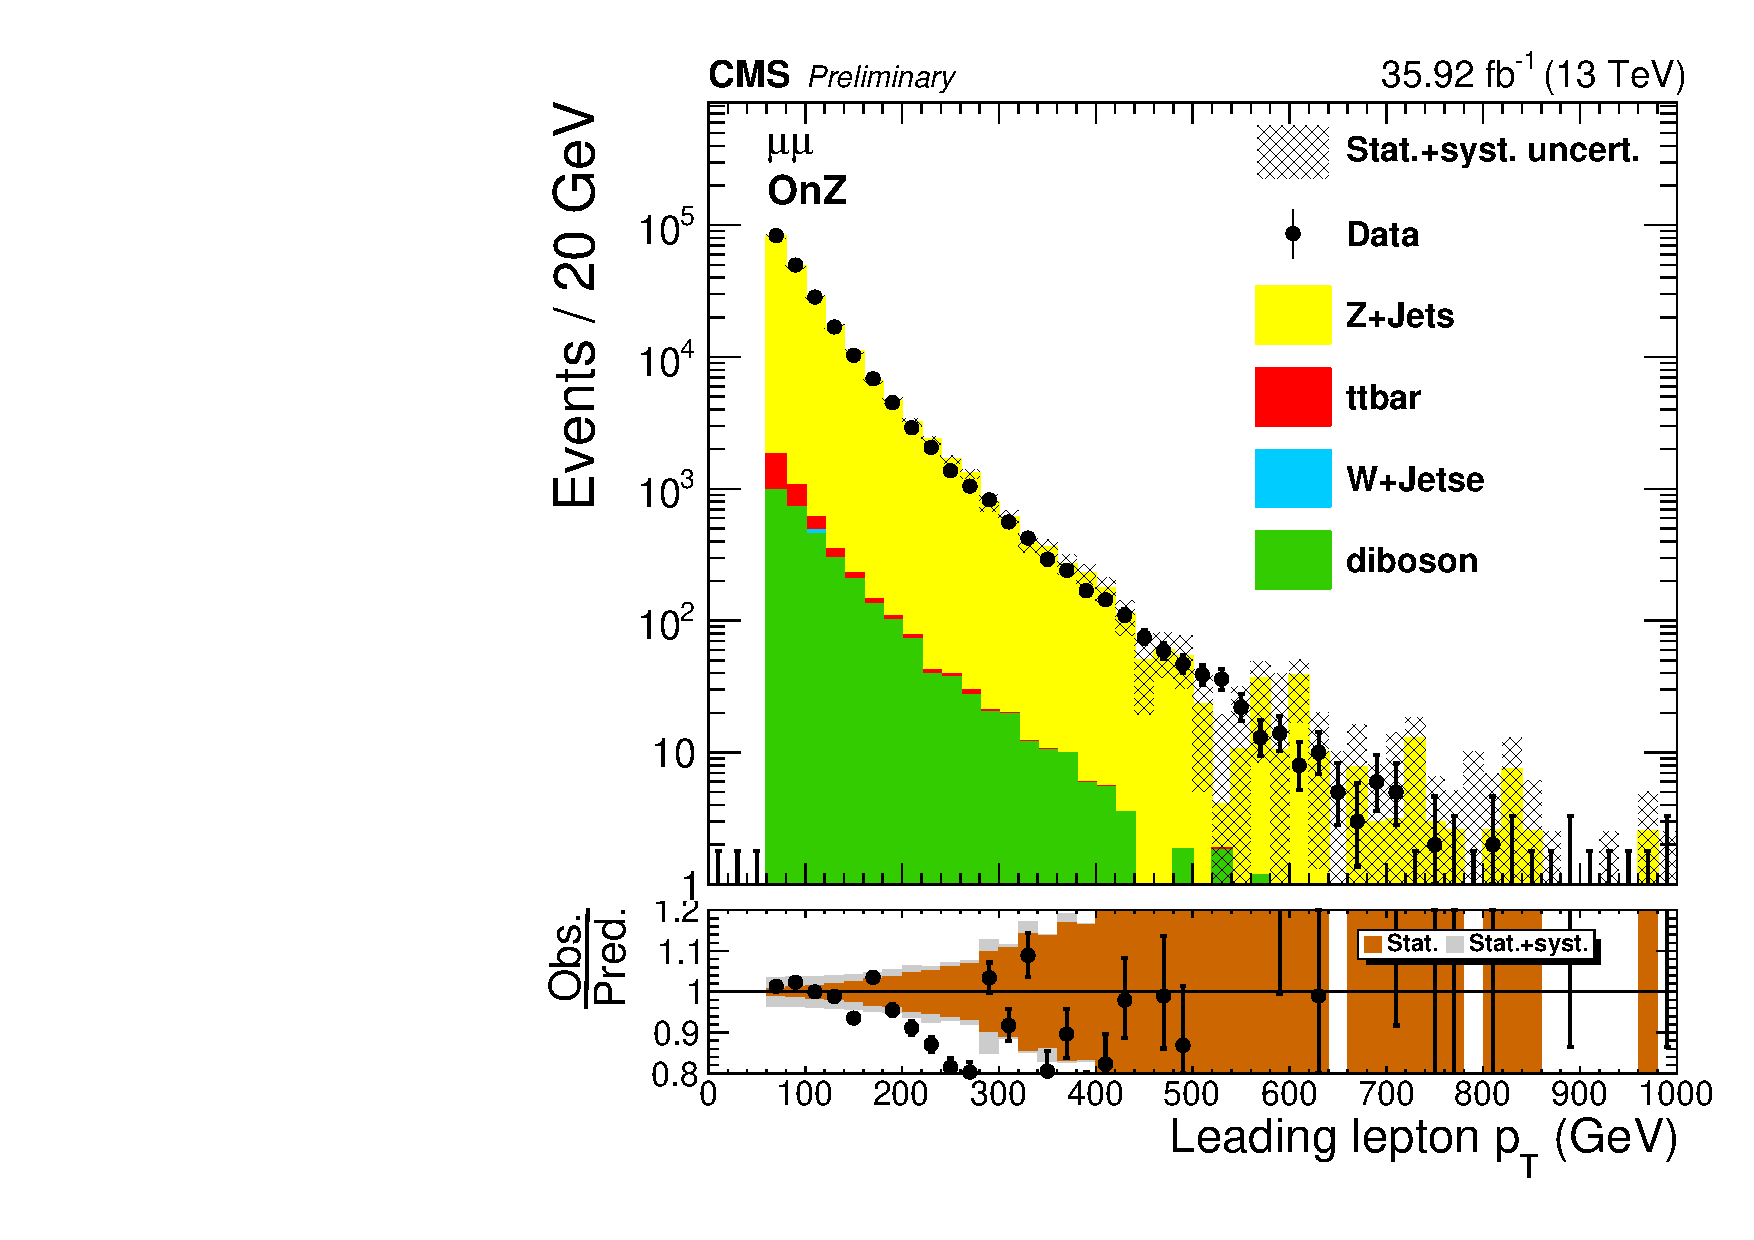
\includegraphics[width=0.45\textwidth]{figures/2016/AfterNormSF_Lepton_0_Pt_HNWR_SingleMuon_OnZ.pdf}
  \vspace{0.01\textwidth}

  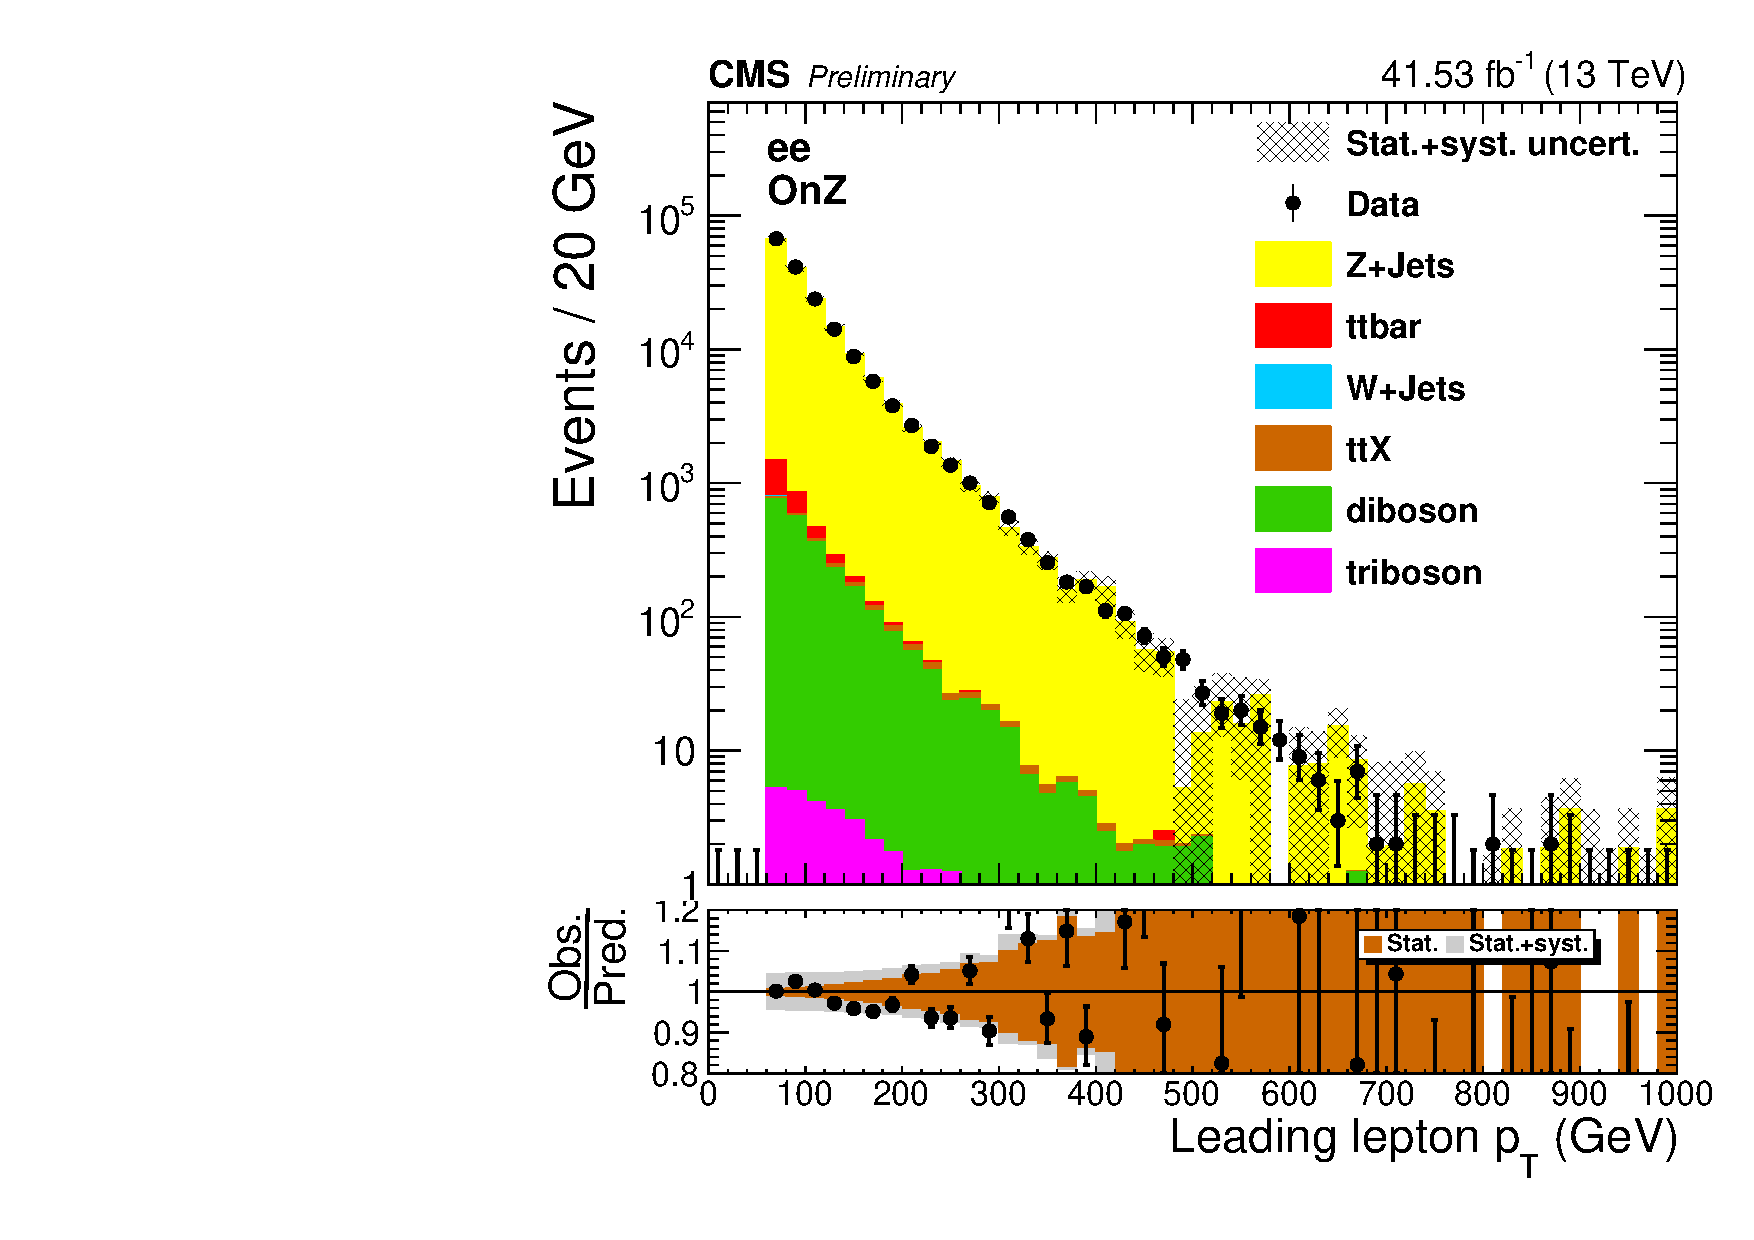
\includegraphics[width=0.45\textwidth]{figures/2017/AfterNormSF_Lepton_0_Pt_HNWR_SingleElectron_OnZ.pdf}
  \hspace{0.01\textwidth}
  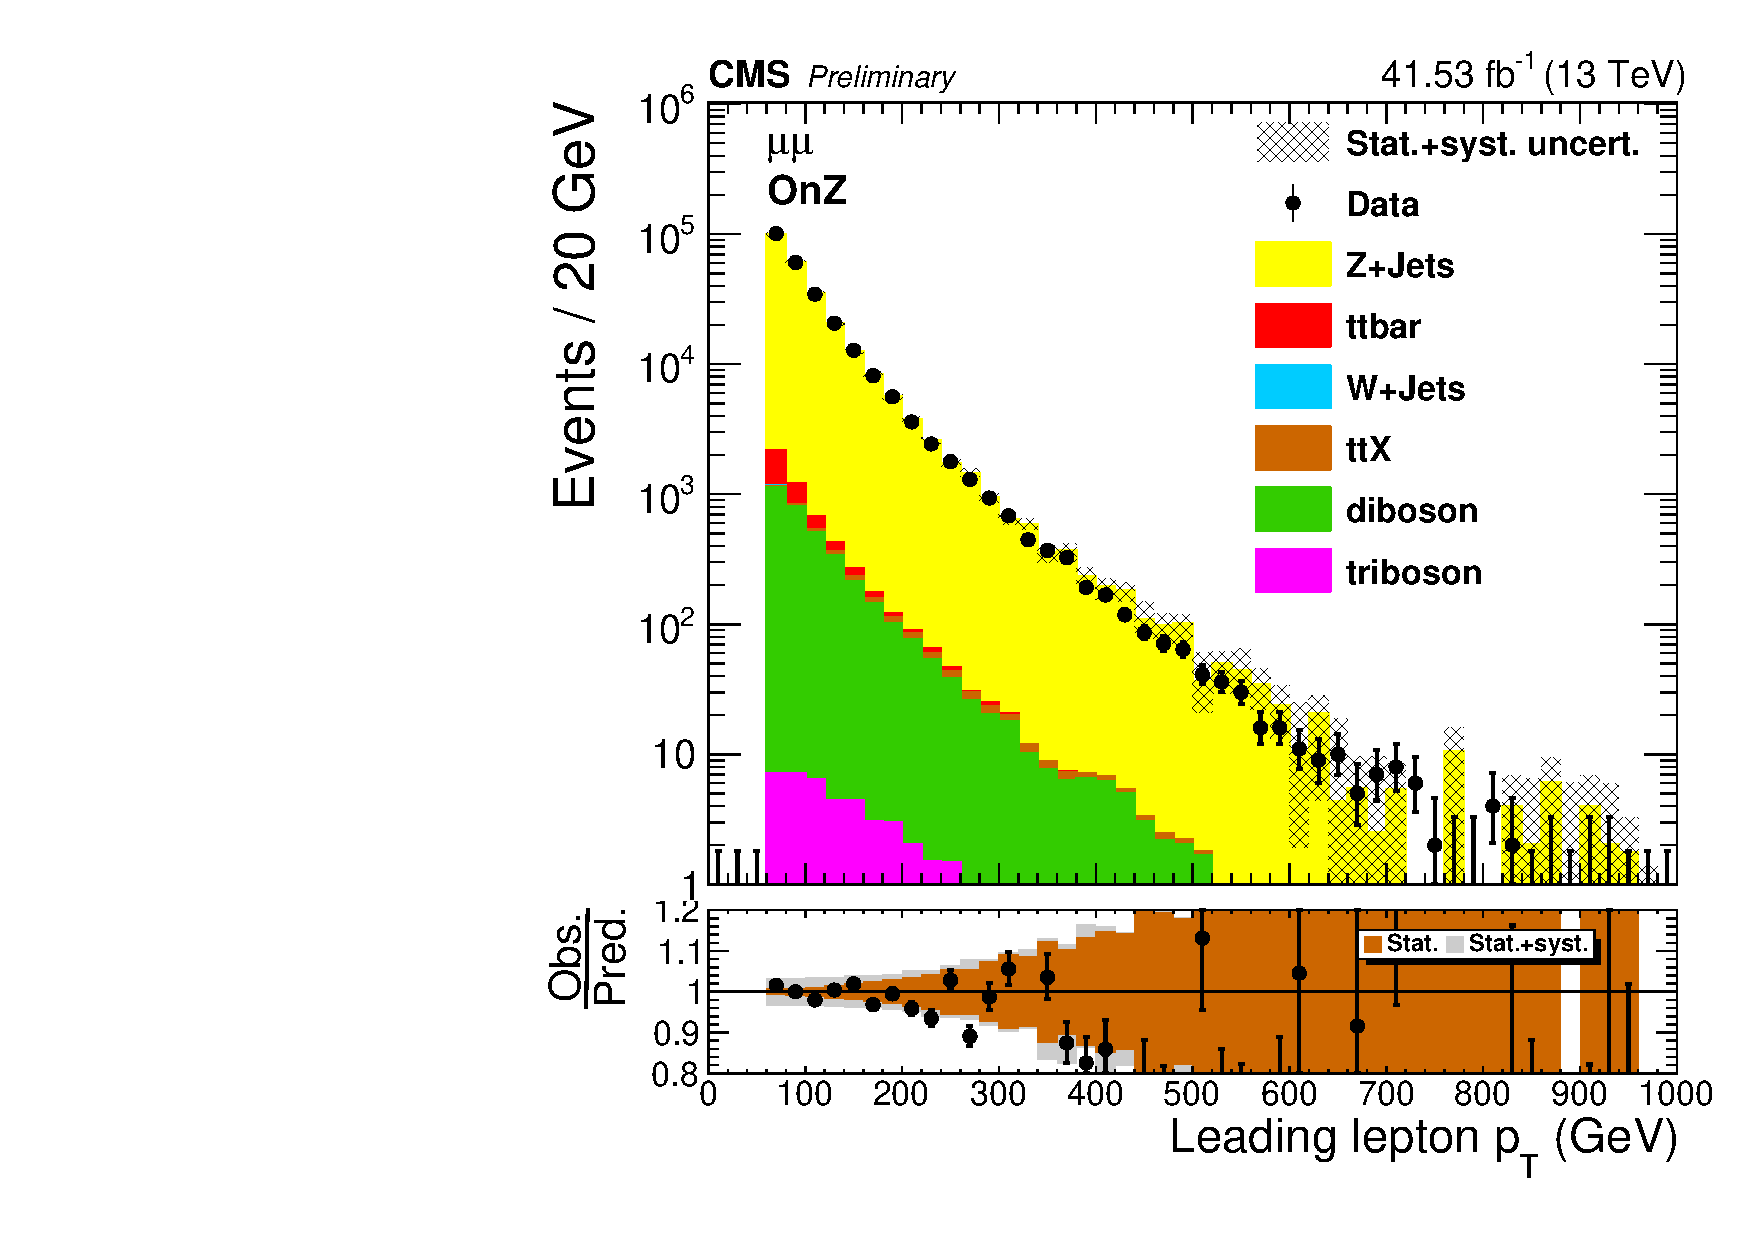
\includegraphics[width=0.45\textwidth]{figures/2017/AfterNormSF_Lepton_0_Pt_HNWR_SingleMuon_OnZ.pdf}
  \vspace{0.01\textwidth}

  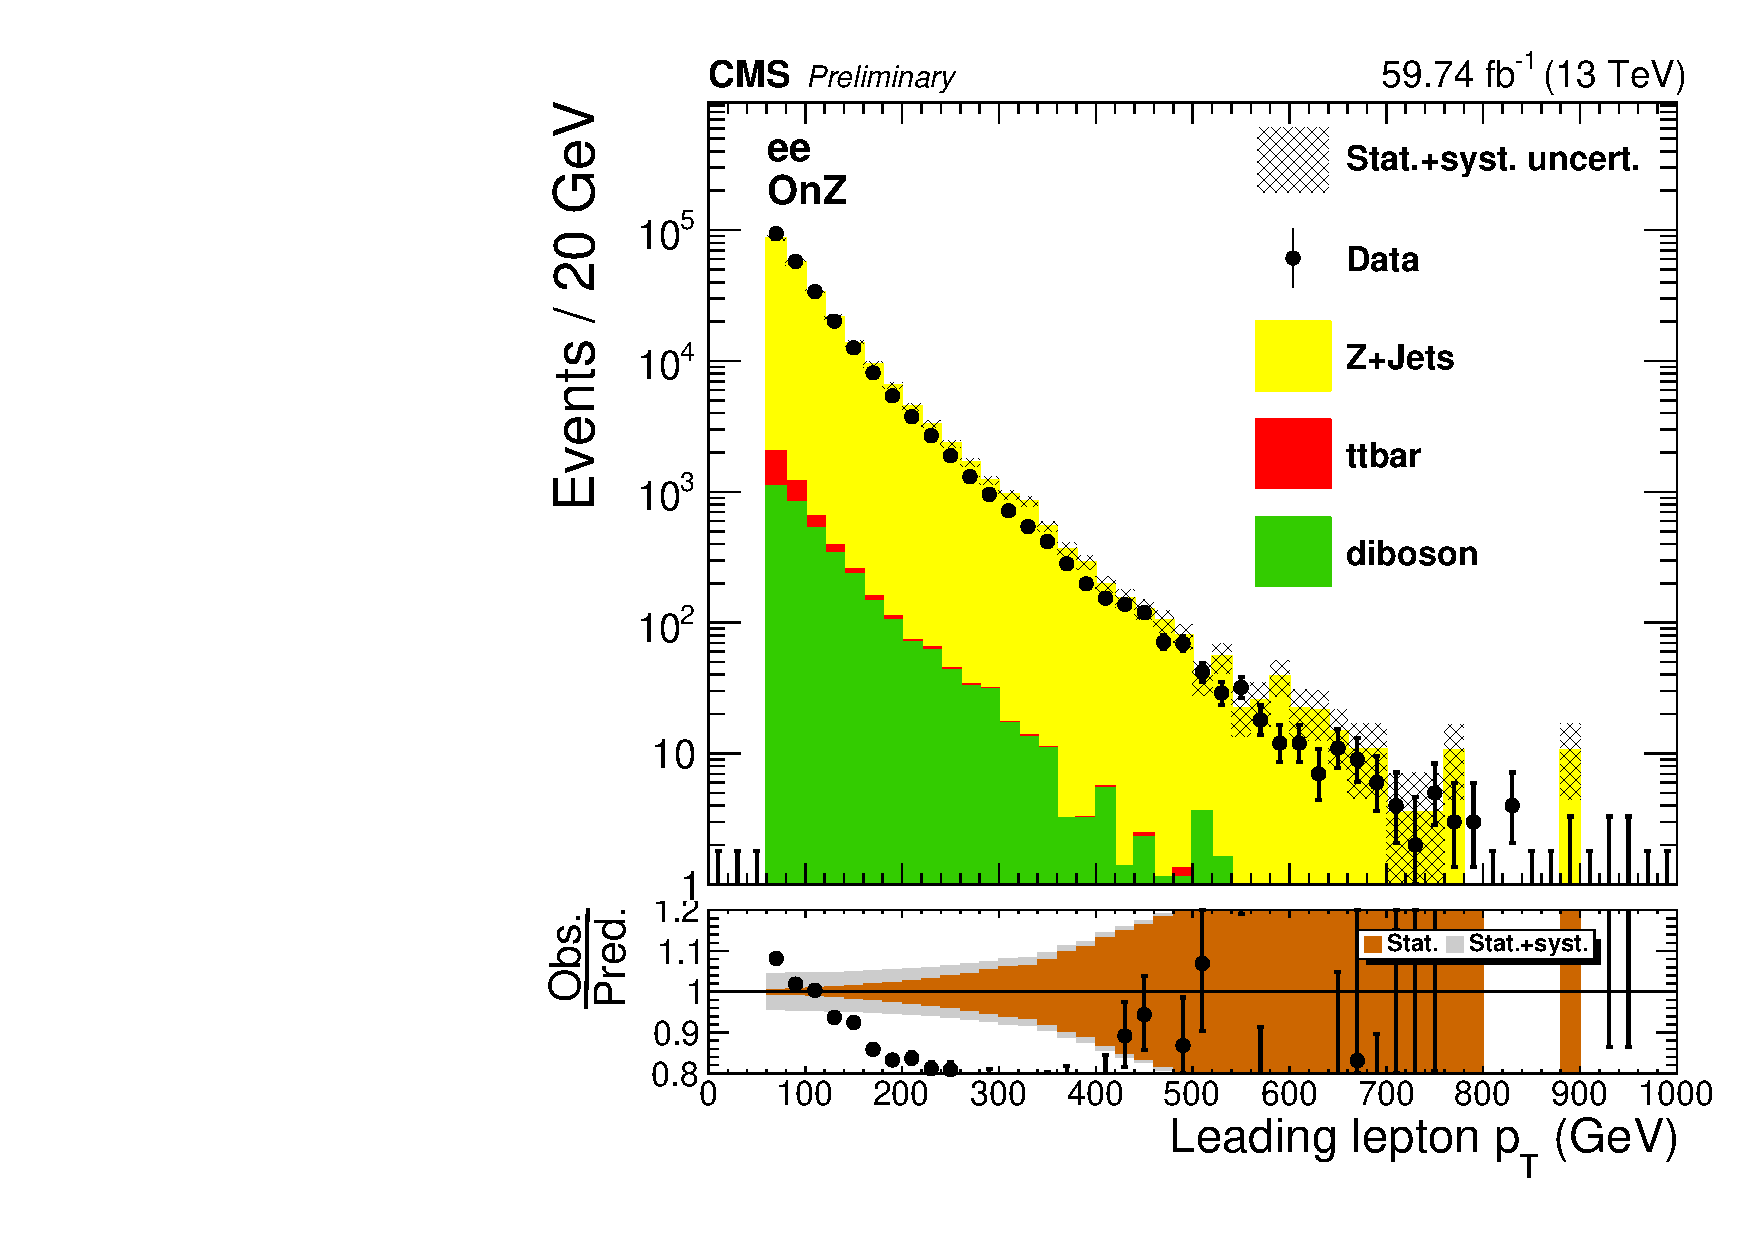
\includegraphics[width=0.45\textwidth]{figures/2018/AfterNormSF_Lepton_0_Pt_HNWR_SingleElectron_OnZ.pdf}
  \hspace{0.01\textwidth}
  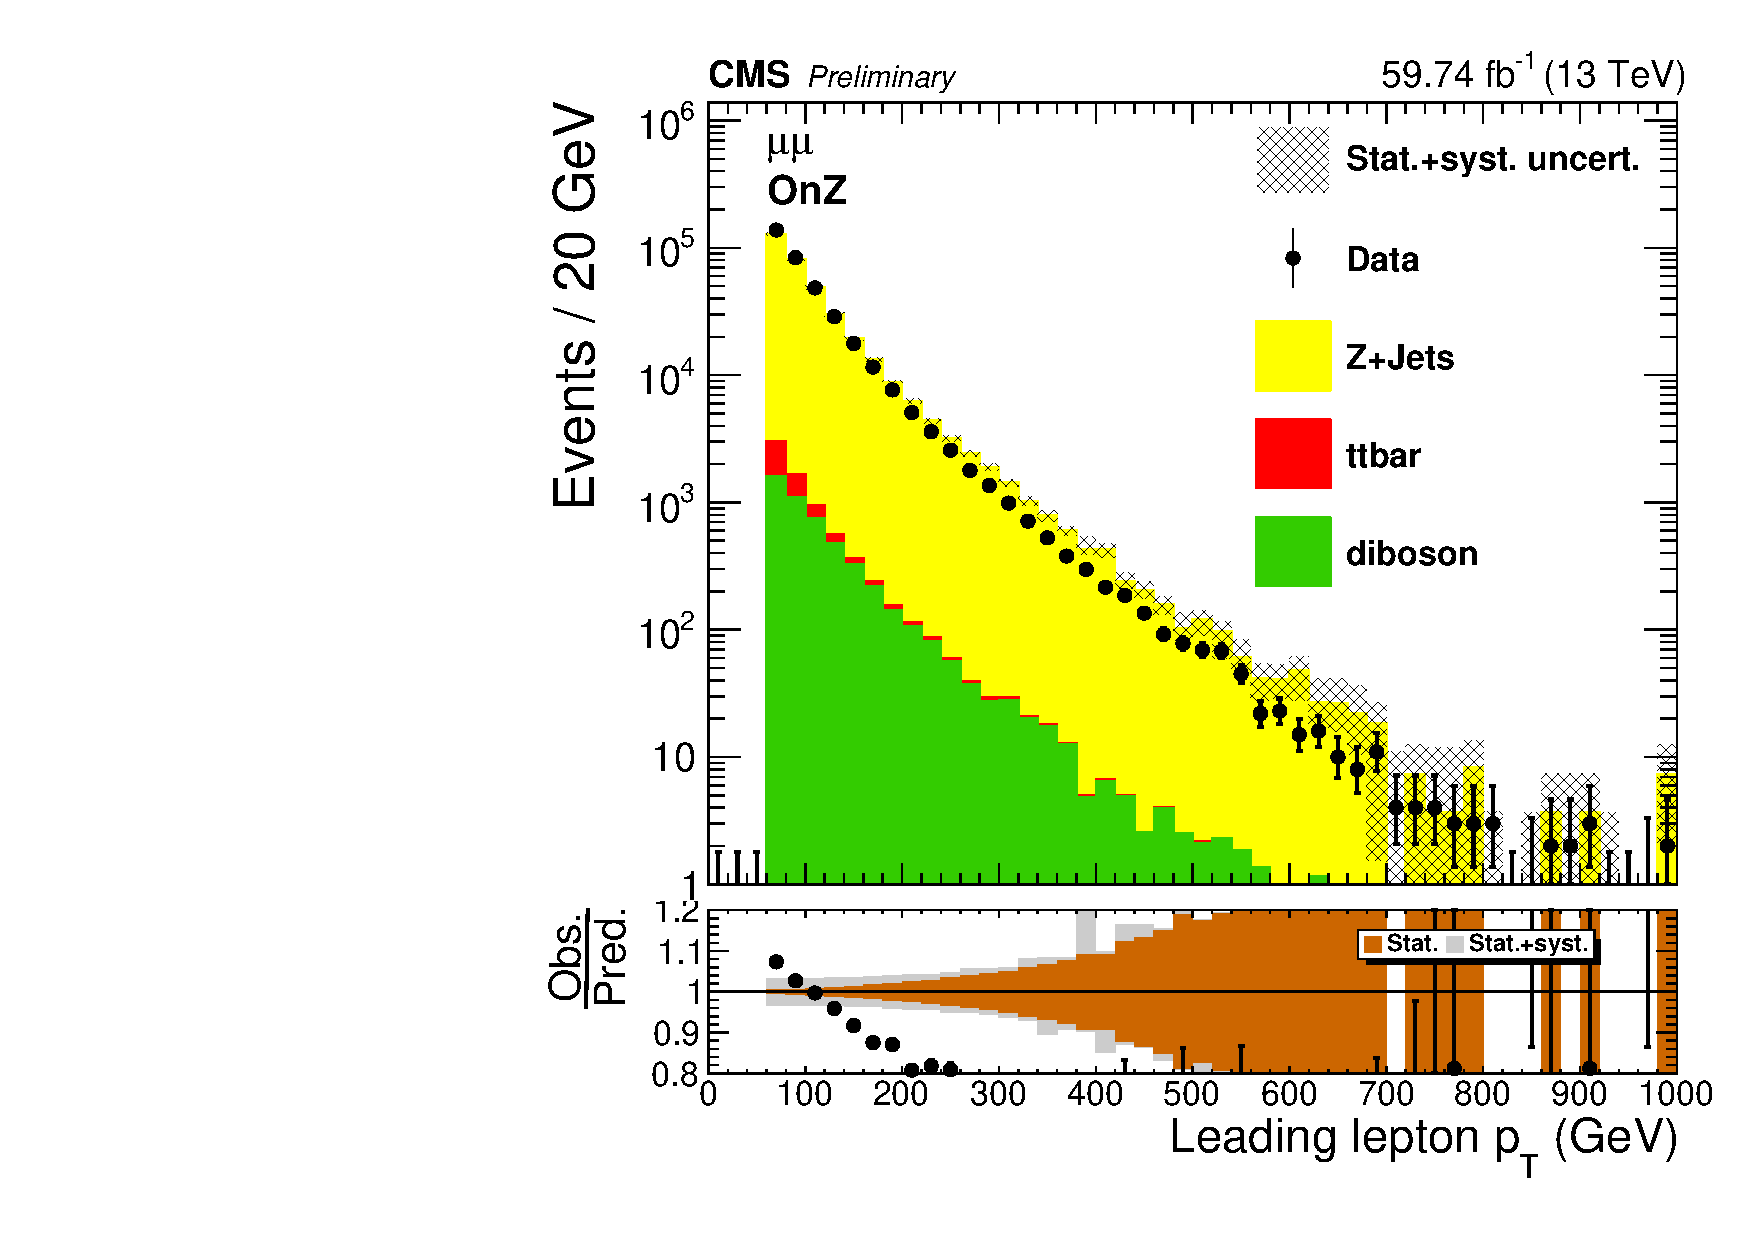
\includegraphics[width=0.45\textwidth]{figures/2018/AfterNormSF_Lepton_0_Pt_HNWR_SingleMuon_OnZ.pdf}

  \topcaption{
    The lepton \pt distributions in the $\PZ$+Jets dominant control region, after applying the normalization scale factors, but not the $\PZ$-$\pt$ reweighting..
    Results for dielectron (dimuon) channel is shown on the left (right), for 2016 (top), 2017 (middle) and 2018 (bottom).
  }
  \label{fig:BkgdZptLepPtBefore}
\end{figure}

\begin{figure}[htbp]
  \centering

  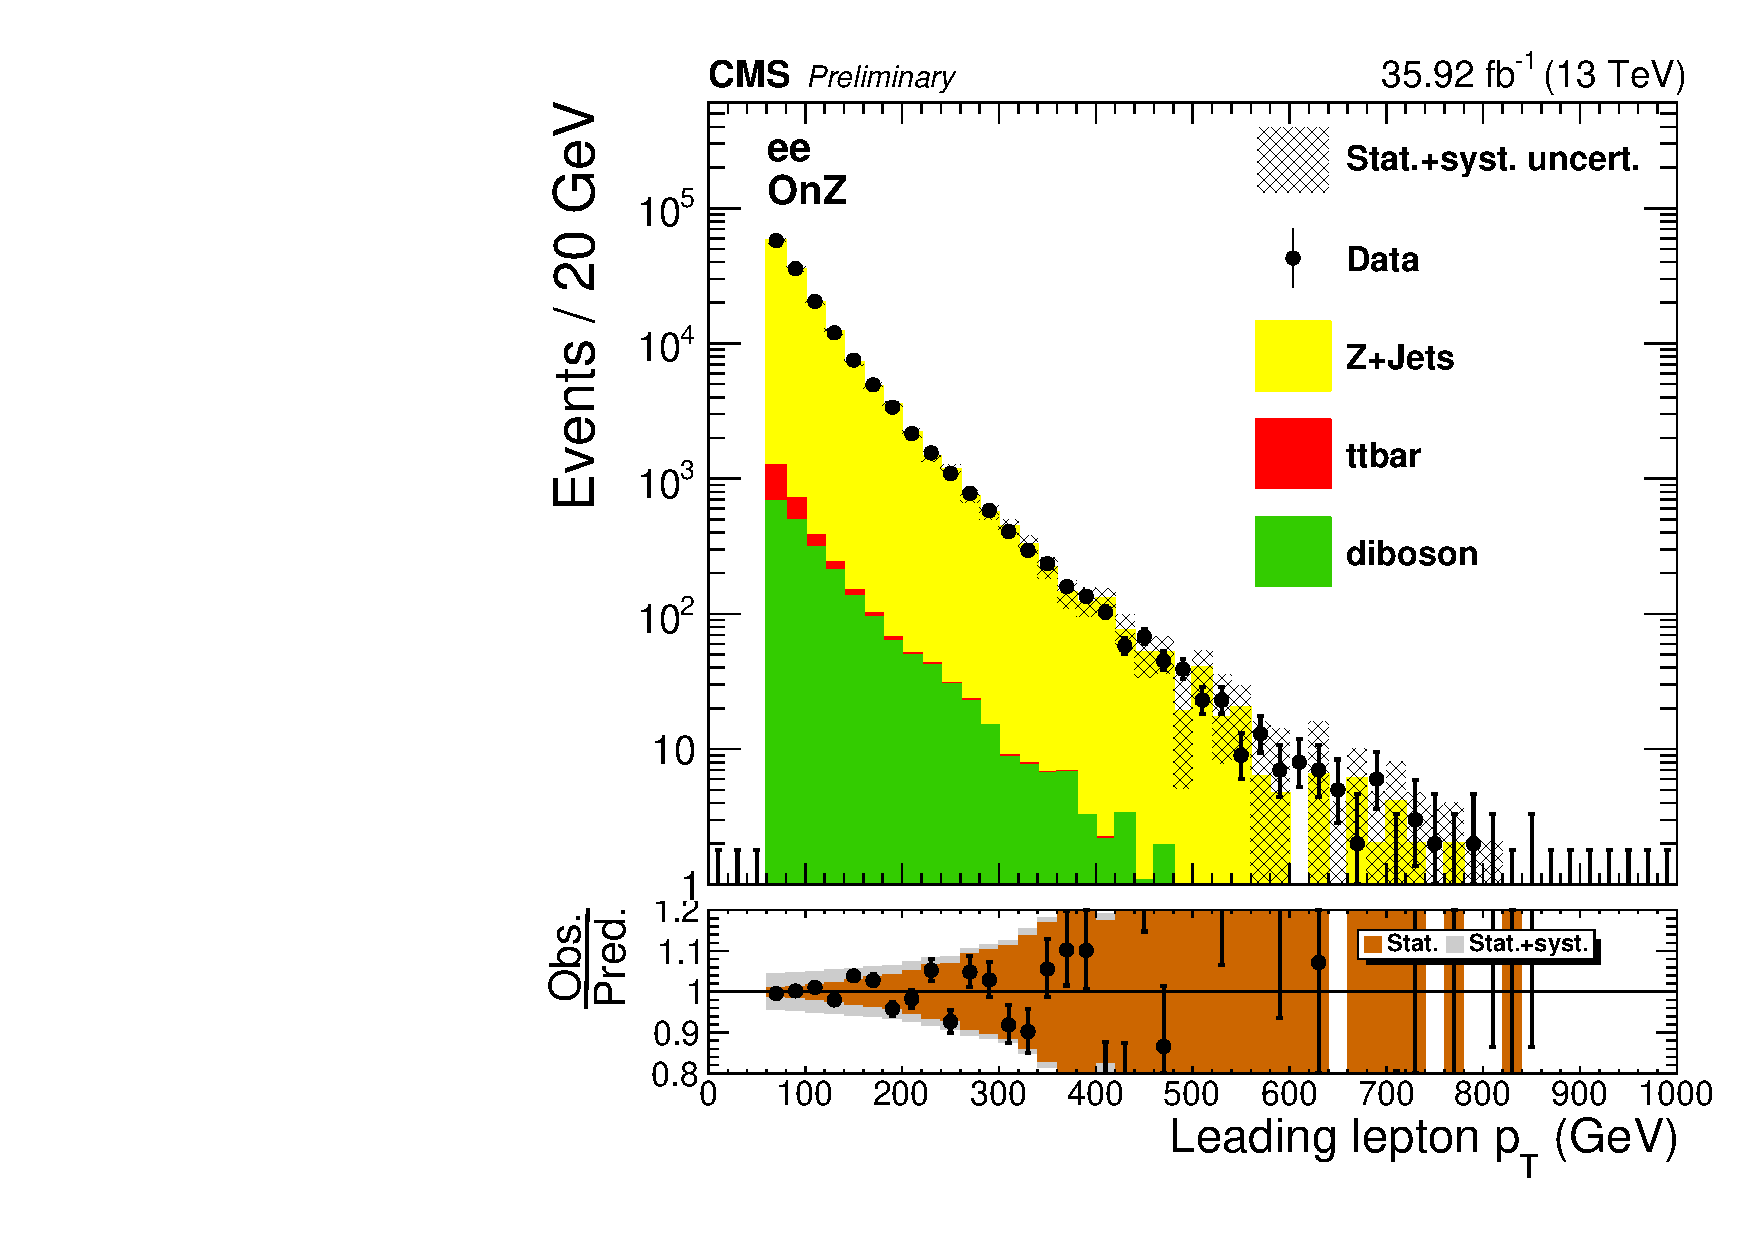
\includegraphics[width=0.45\textwidth]{figures/2016/AfterNormSFAndZPtReweighting_Lepton_0_Pt_HNWR_SingleElectron_OnZ.pdf}
  \hspace{0.01\textwidth}
  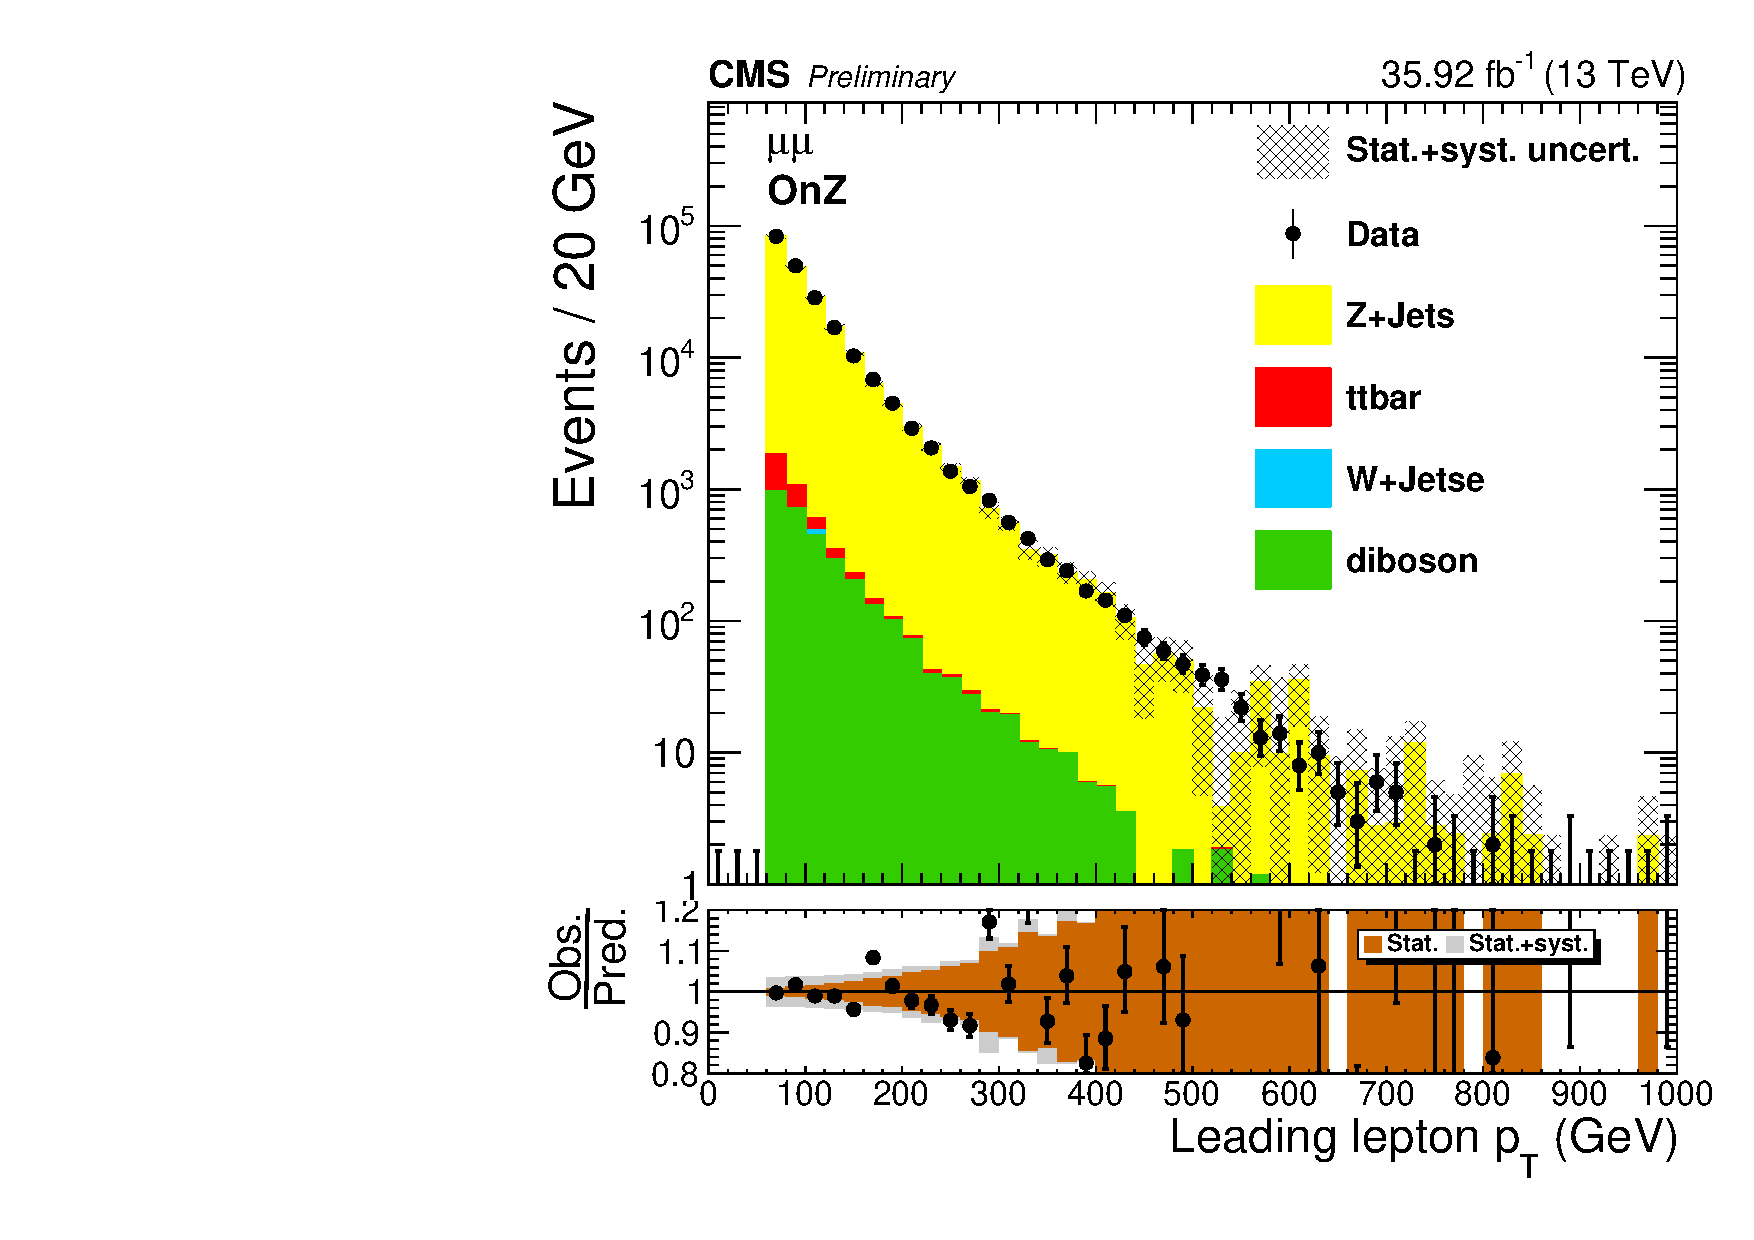
\includegraphics[width=0.45\textwidth]{figures/2016/AfterNormSFAndZPtReweighting_Lepton_0_Pt_HNWR_SingleMuon_OnZ.pdf}
  \vspace{0.01\textwidth}

  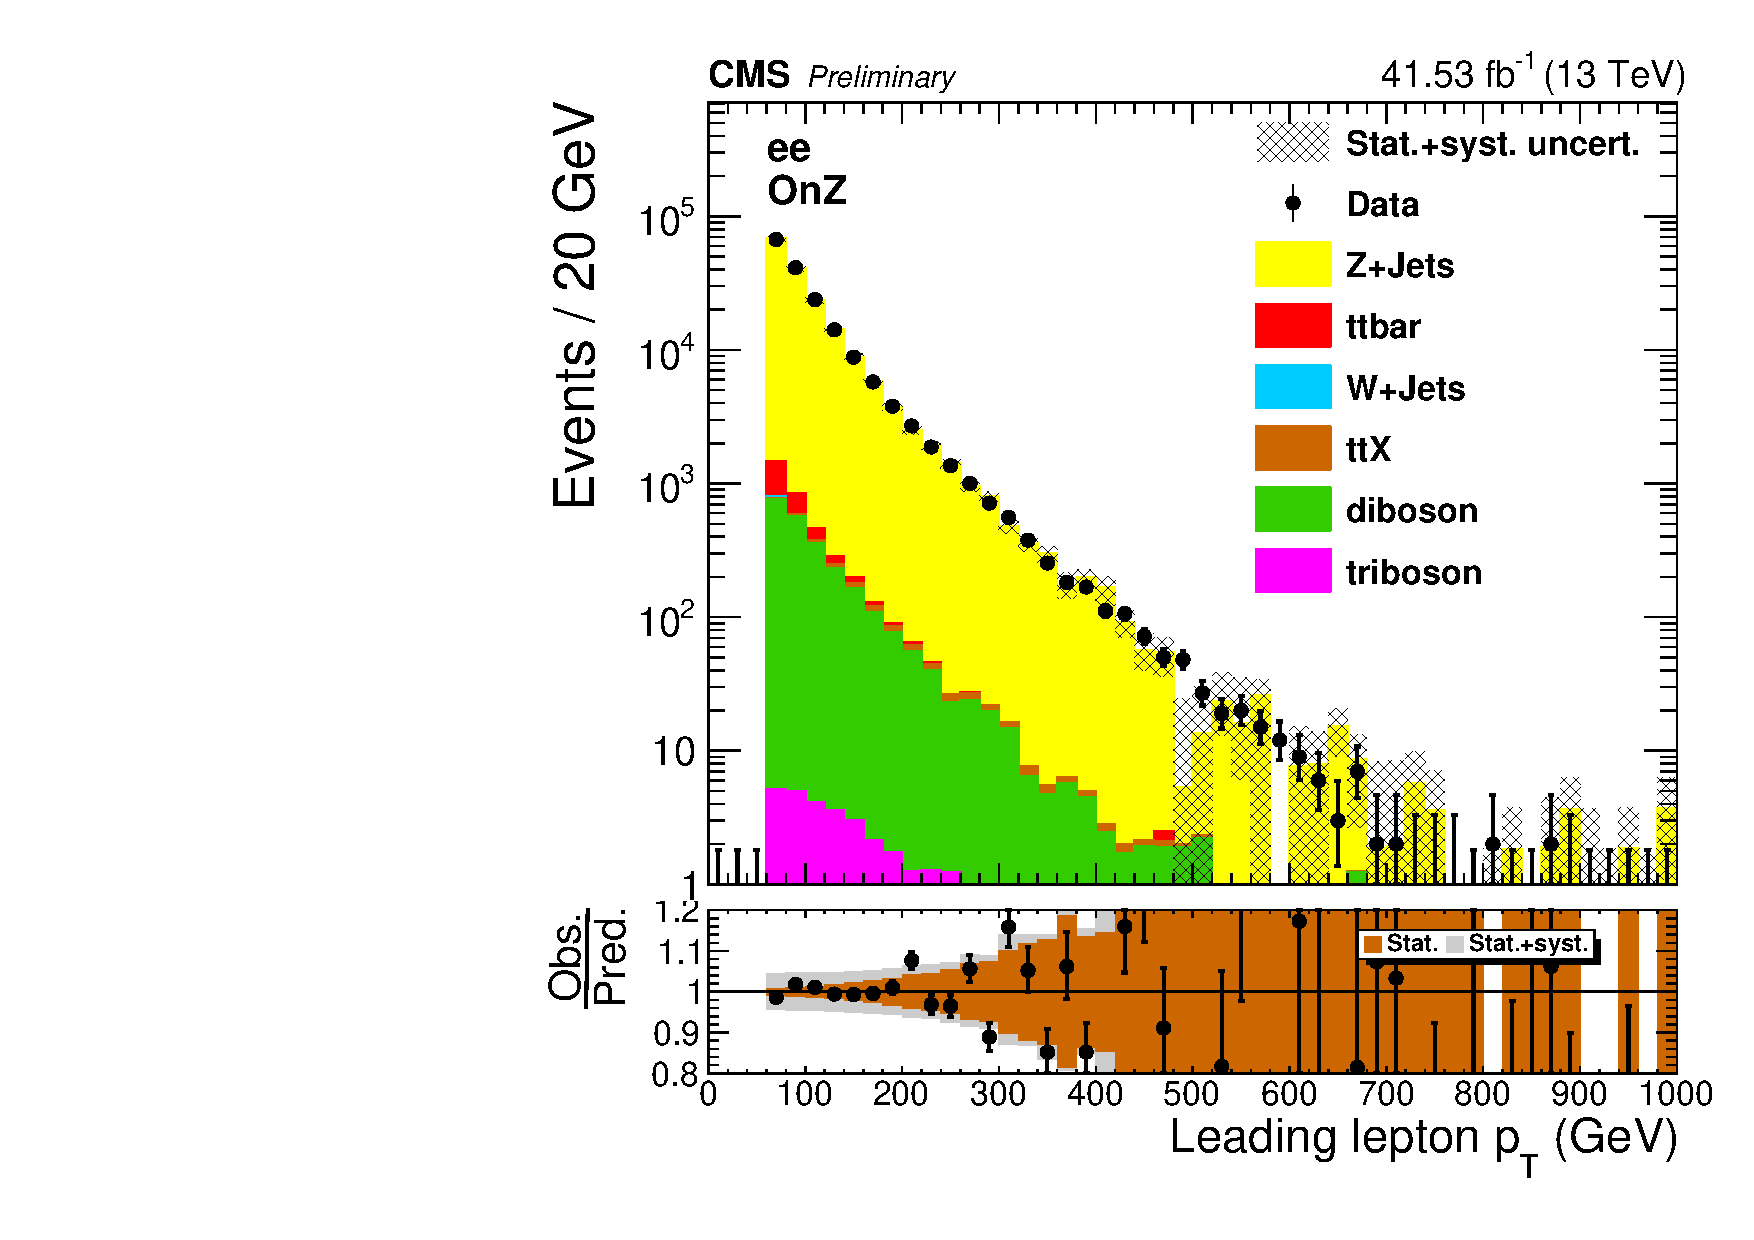
\includegraphics[width=0.45\textwidth]{figures/2017/AfterNormSFAndZPtReweighting_Lepton_0_Pt_HNWR_SingleElectron_OnZ.pdf}
  \hspace{0.01\textwidth}
  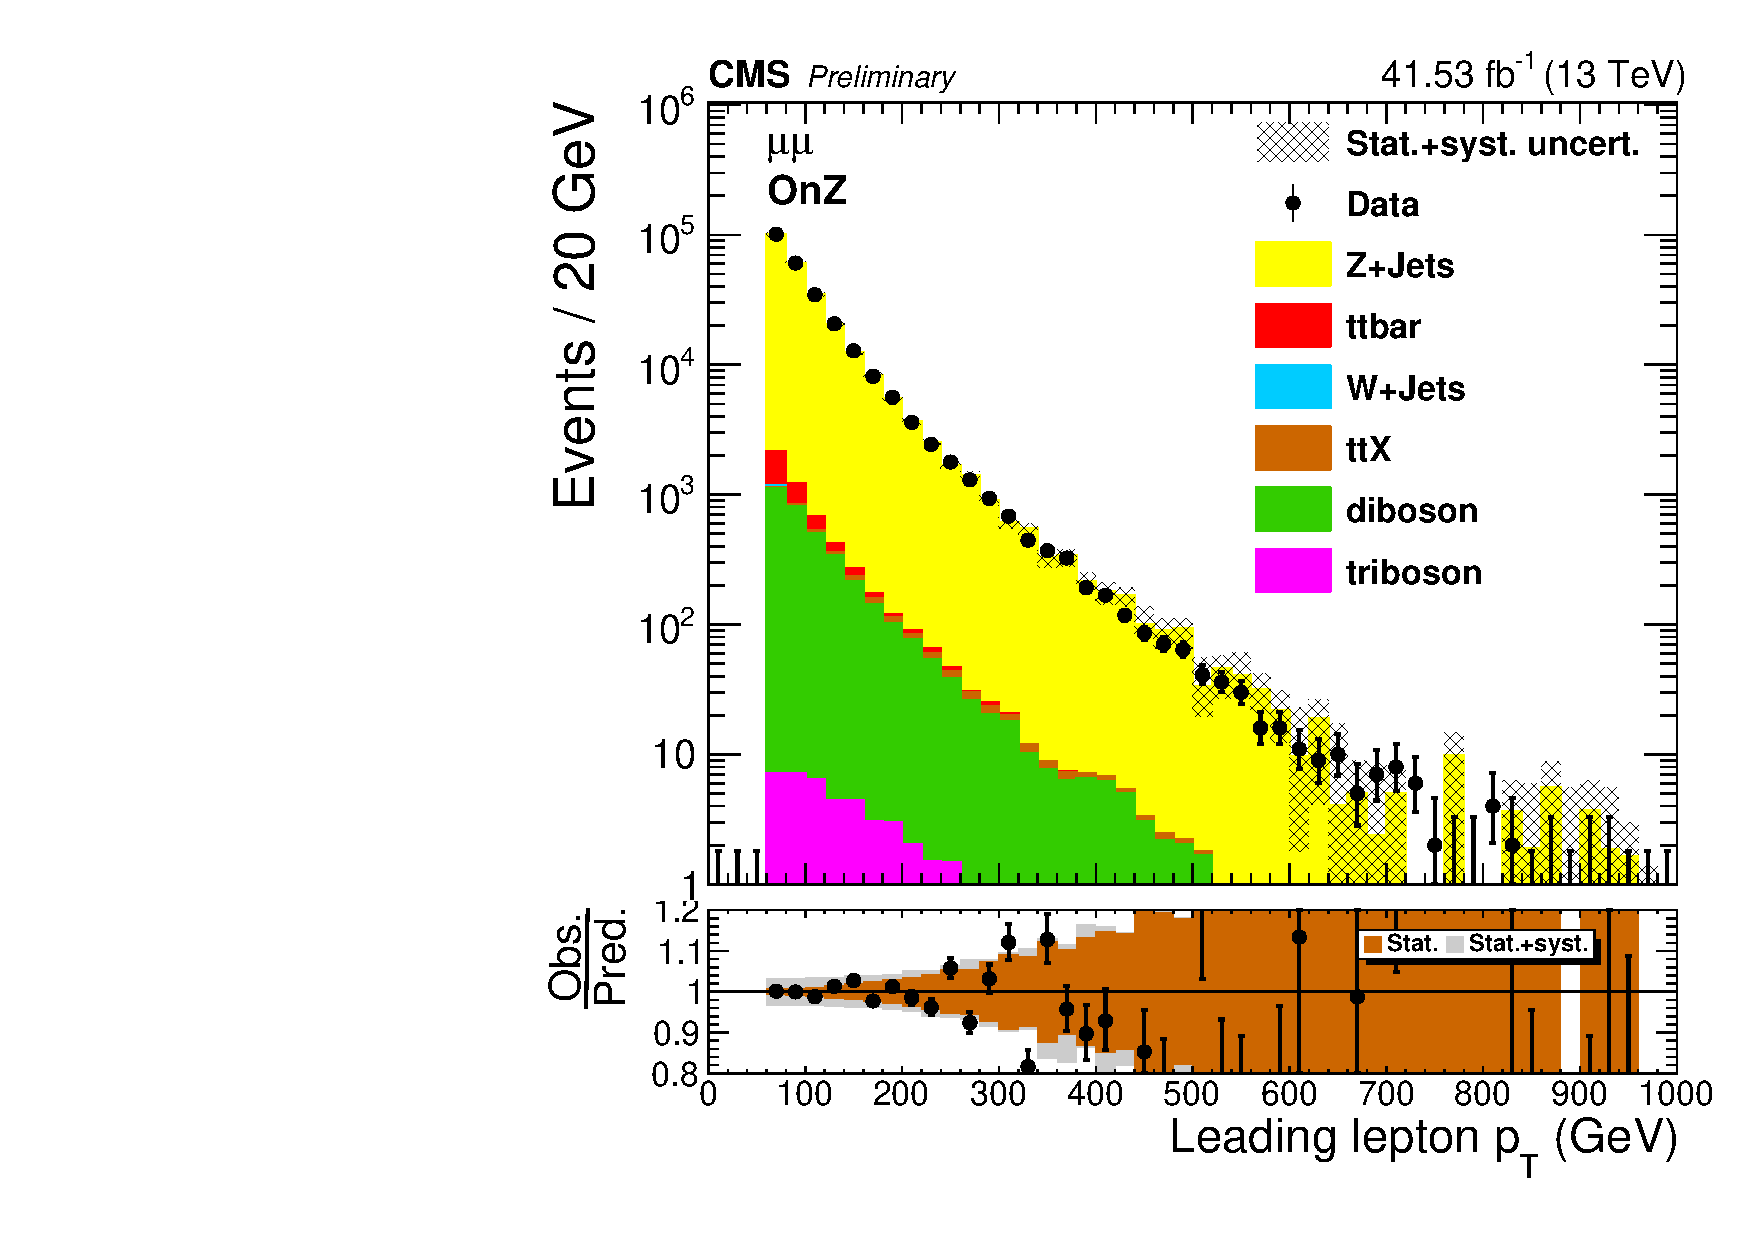
\includegraphics[width=0.45\textwidth]{figures/2017/AfterNormSFAndZPtReweighting_Lepton_0_Pt_HNWR_SingleMuon_OnZ.pdf}
  \vspace{0.01\textwidth}
   
  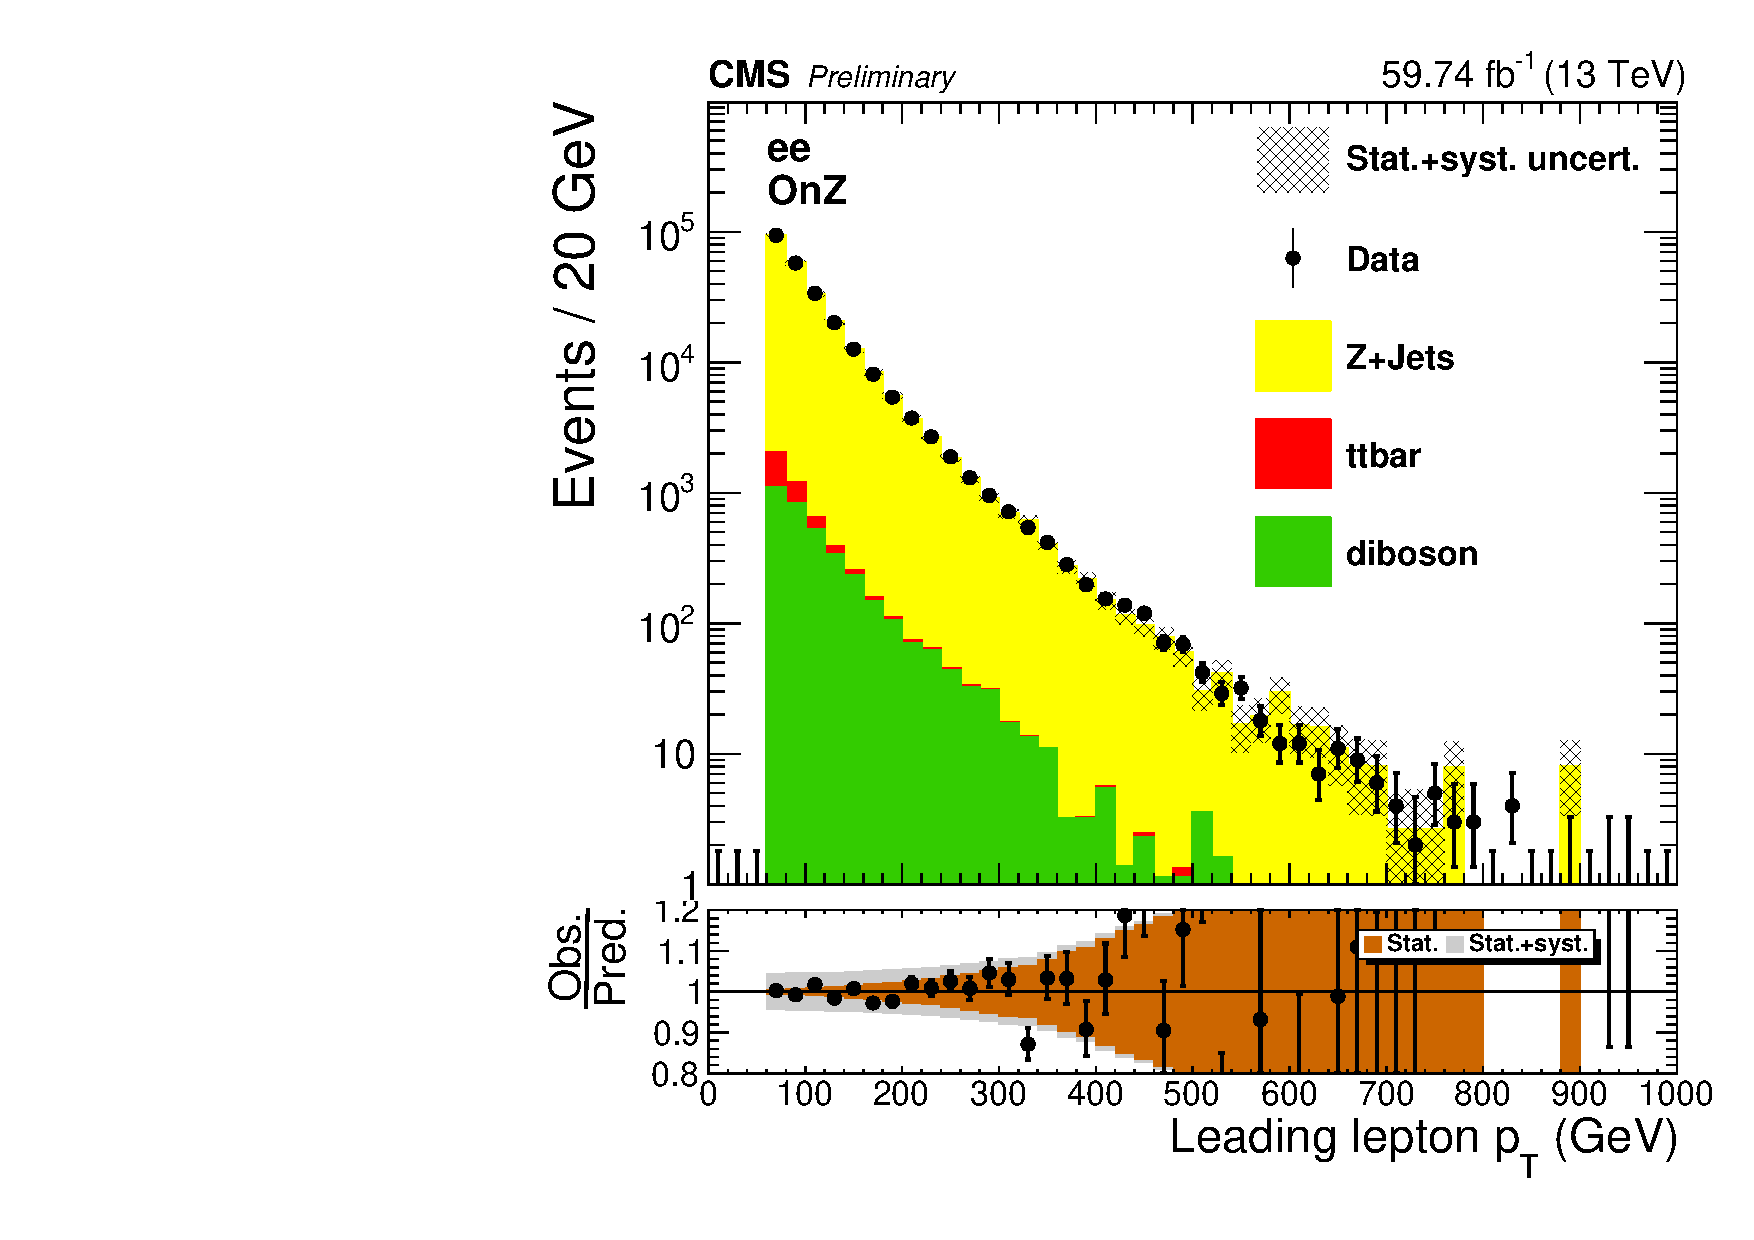
\includegraphics[width=0.45\textwidth]{figures/2018/AfterNormSFAndZPtReweighting_Lepton_0_Pt_HNWR_SingleElectron_OnZ.pdf}
  \hspace{0.01\textwidth}
  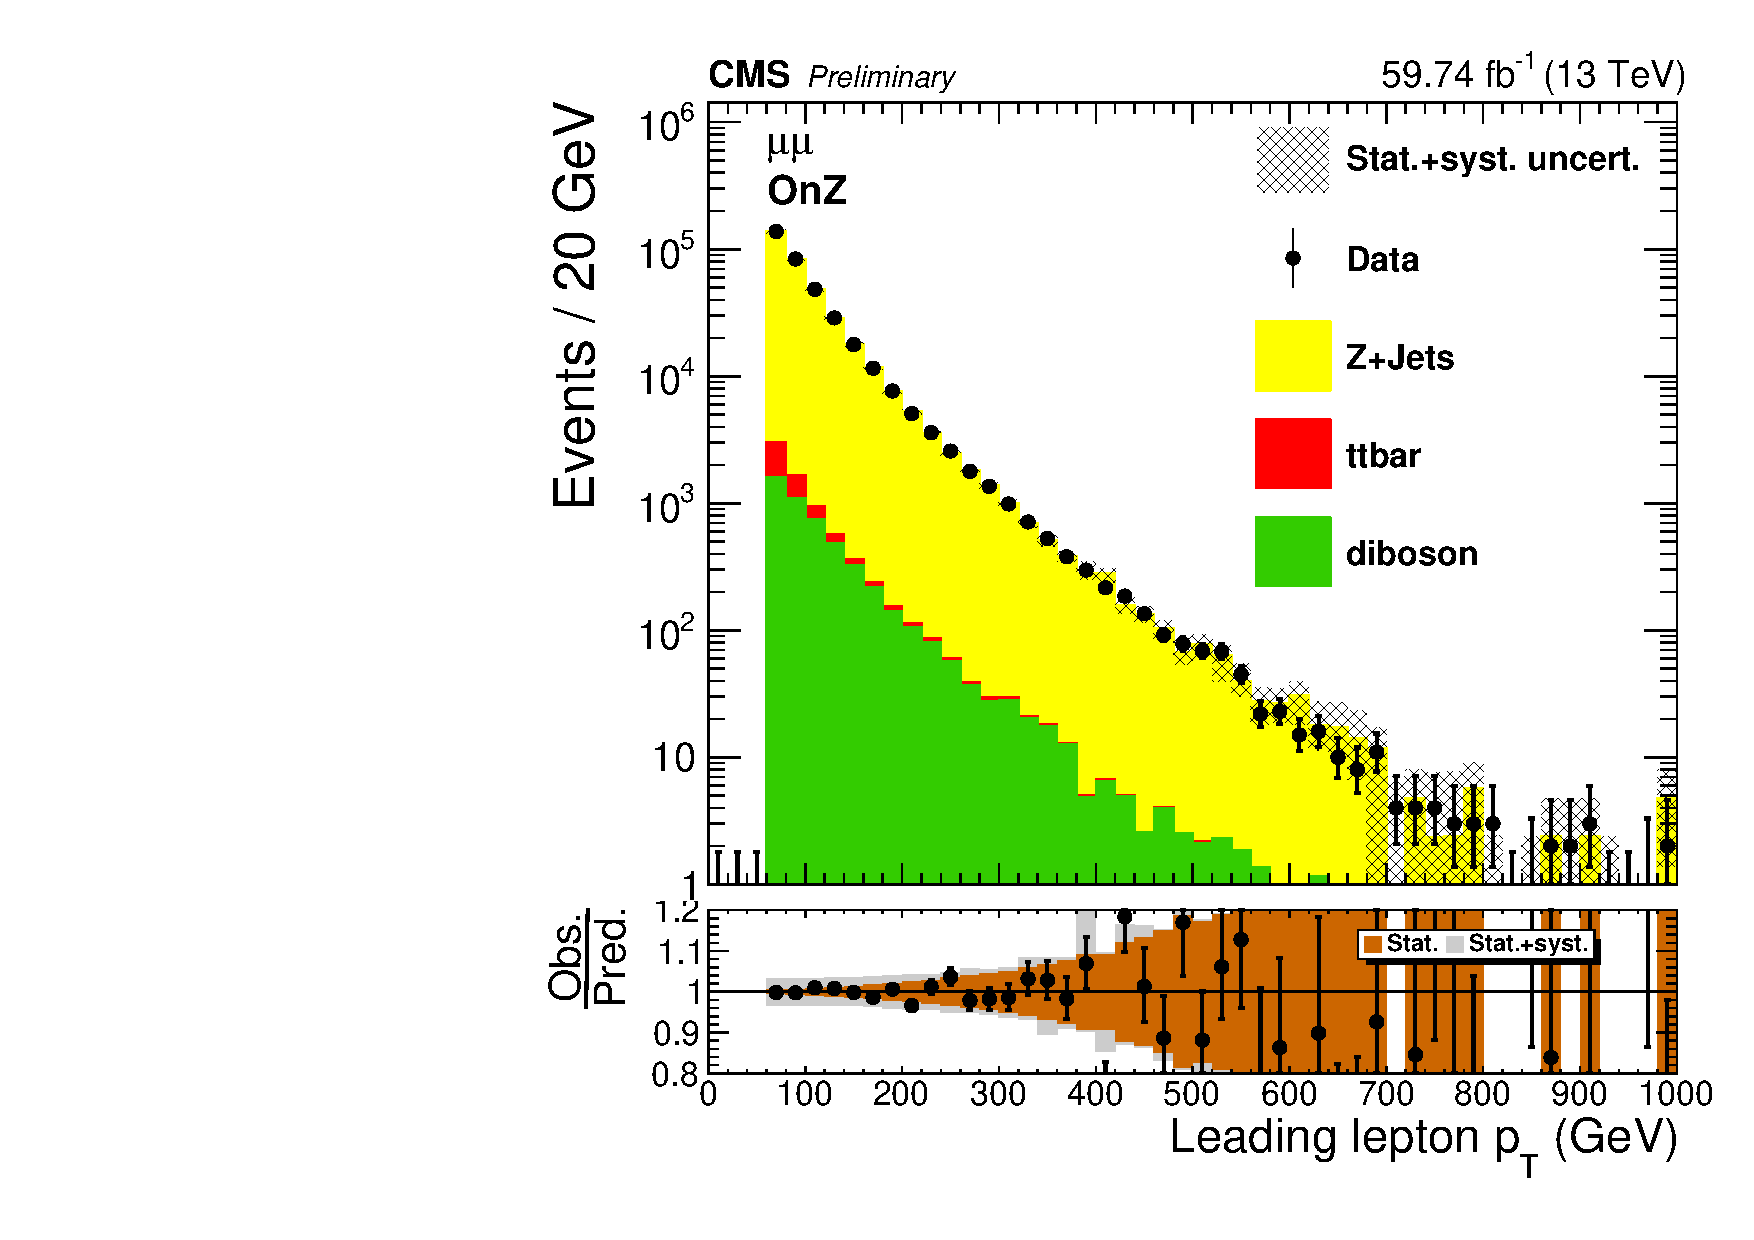
\includegraphics[width=0.45\textwidth]{figures/2018/AfterNormSFAndZPtReweighting_Lepton_0_Pt_HNWR_SingleMuon_OnZ.pdf}


  \topcaption{
    The lepton \pt distributions in the $\PZ$+Jets dominant control region, after applying the normalization scale factors and $\PZ$-$\pt$ reweighting.
    Results for dielectron (dimuon) channel is shown on the left (right), for 2016 (top), 2017 (middle) and 2018 (bottom).
  }
  \label{fig:BkgdZptLepPtAfter}
\end{figure}

The comparison between before and after applying $\PZ$-$\pt$ reweighting in the signal regions are shown in Figs.~\ref{fig:BkgdZptSRCompResolved}--\ref{fig:BkgdZptSRCompBoosted}.

\begin{figure}[htbp]
  \centering

  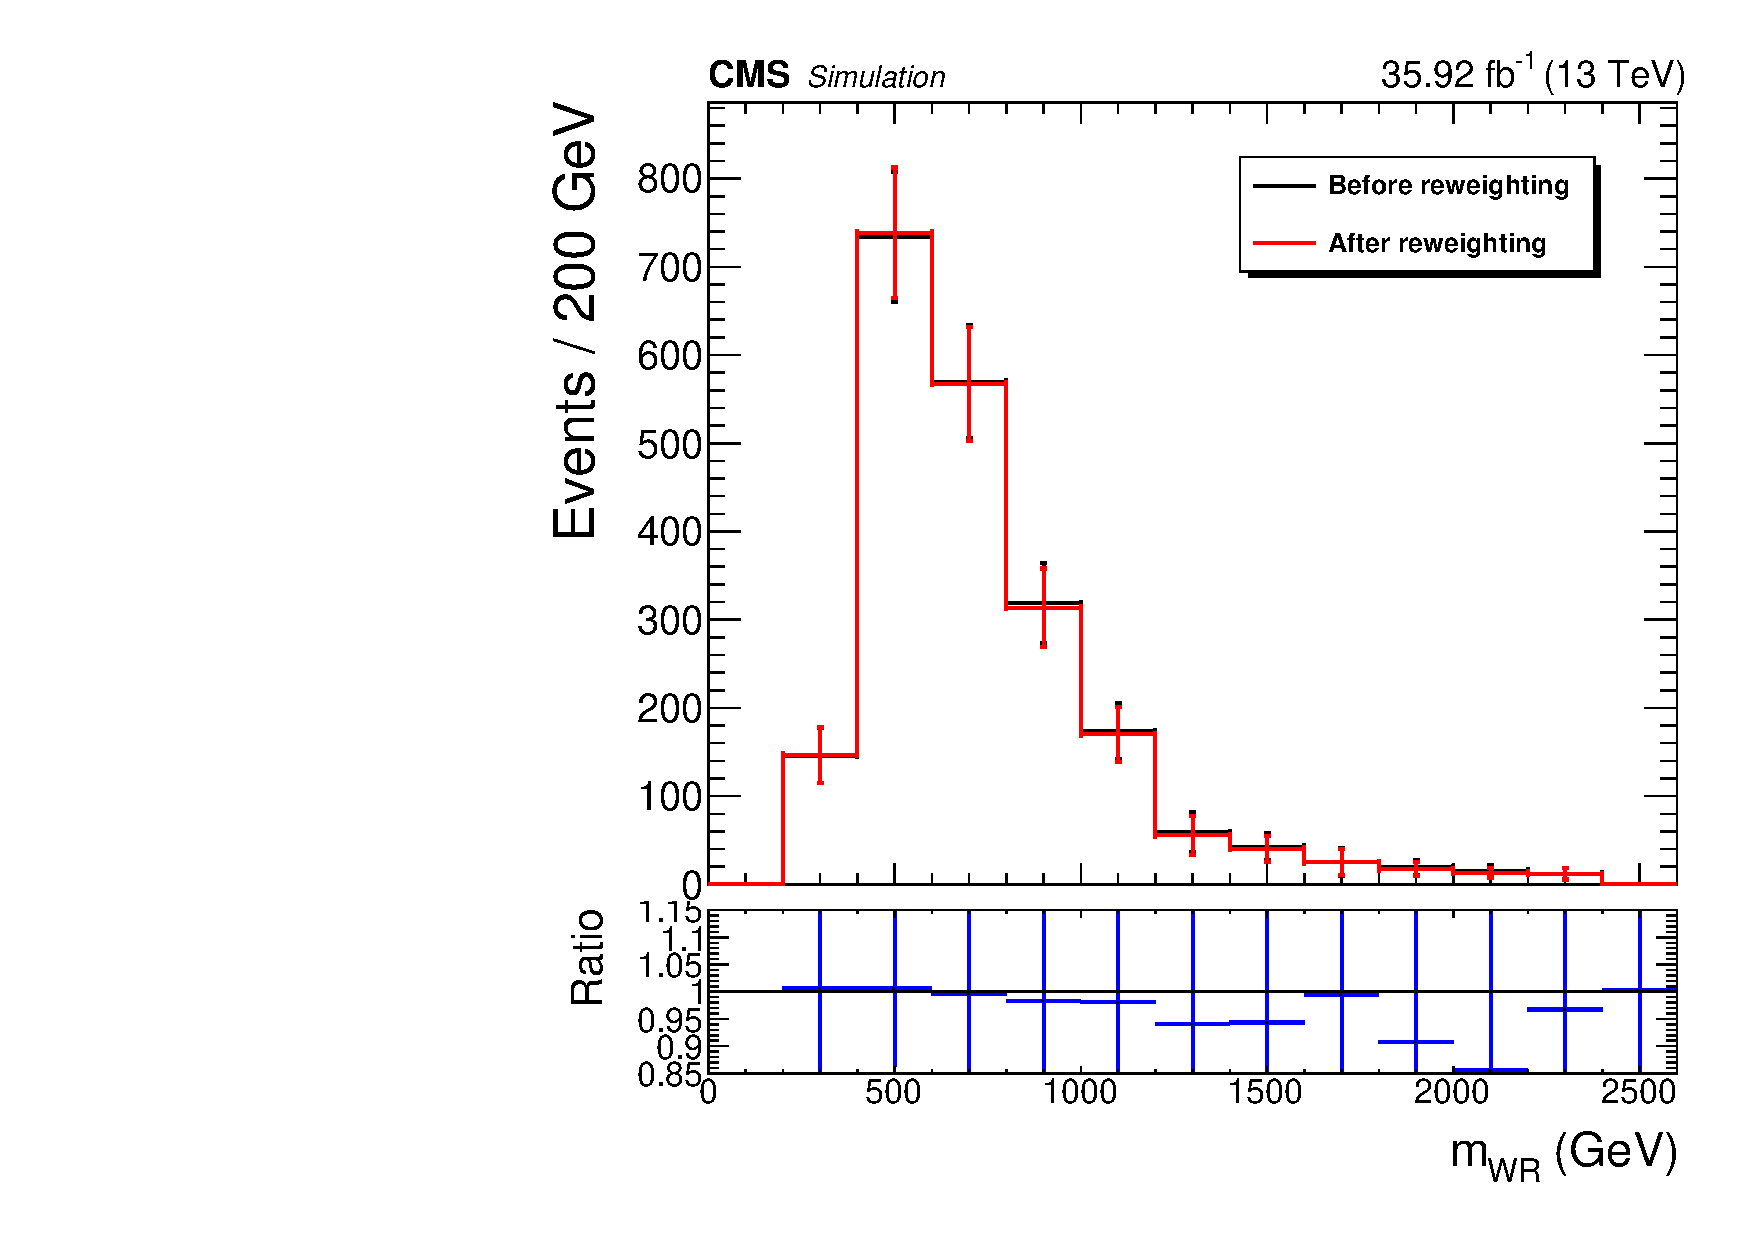
\includegraphics[width=0.45\textwidth]{figures/2016/Resolved_SR_Electron_WRCand_Mass.pdf}
  \hspace{0.01\textwidth}
  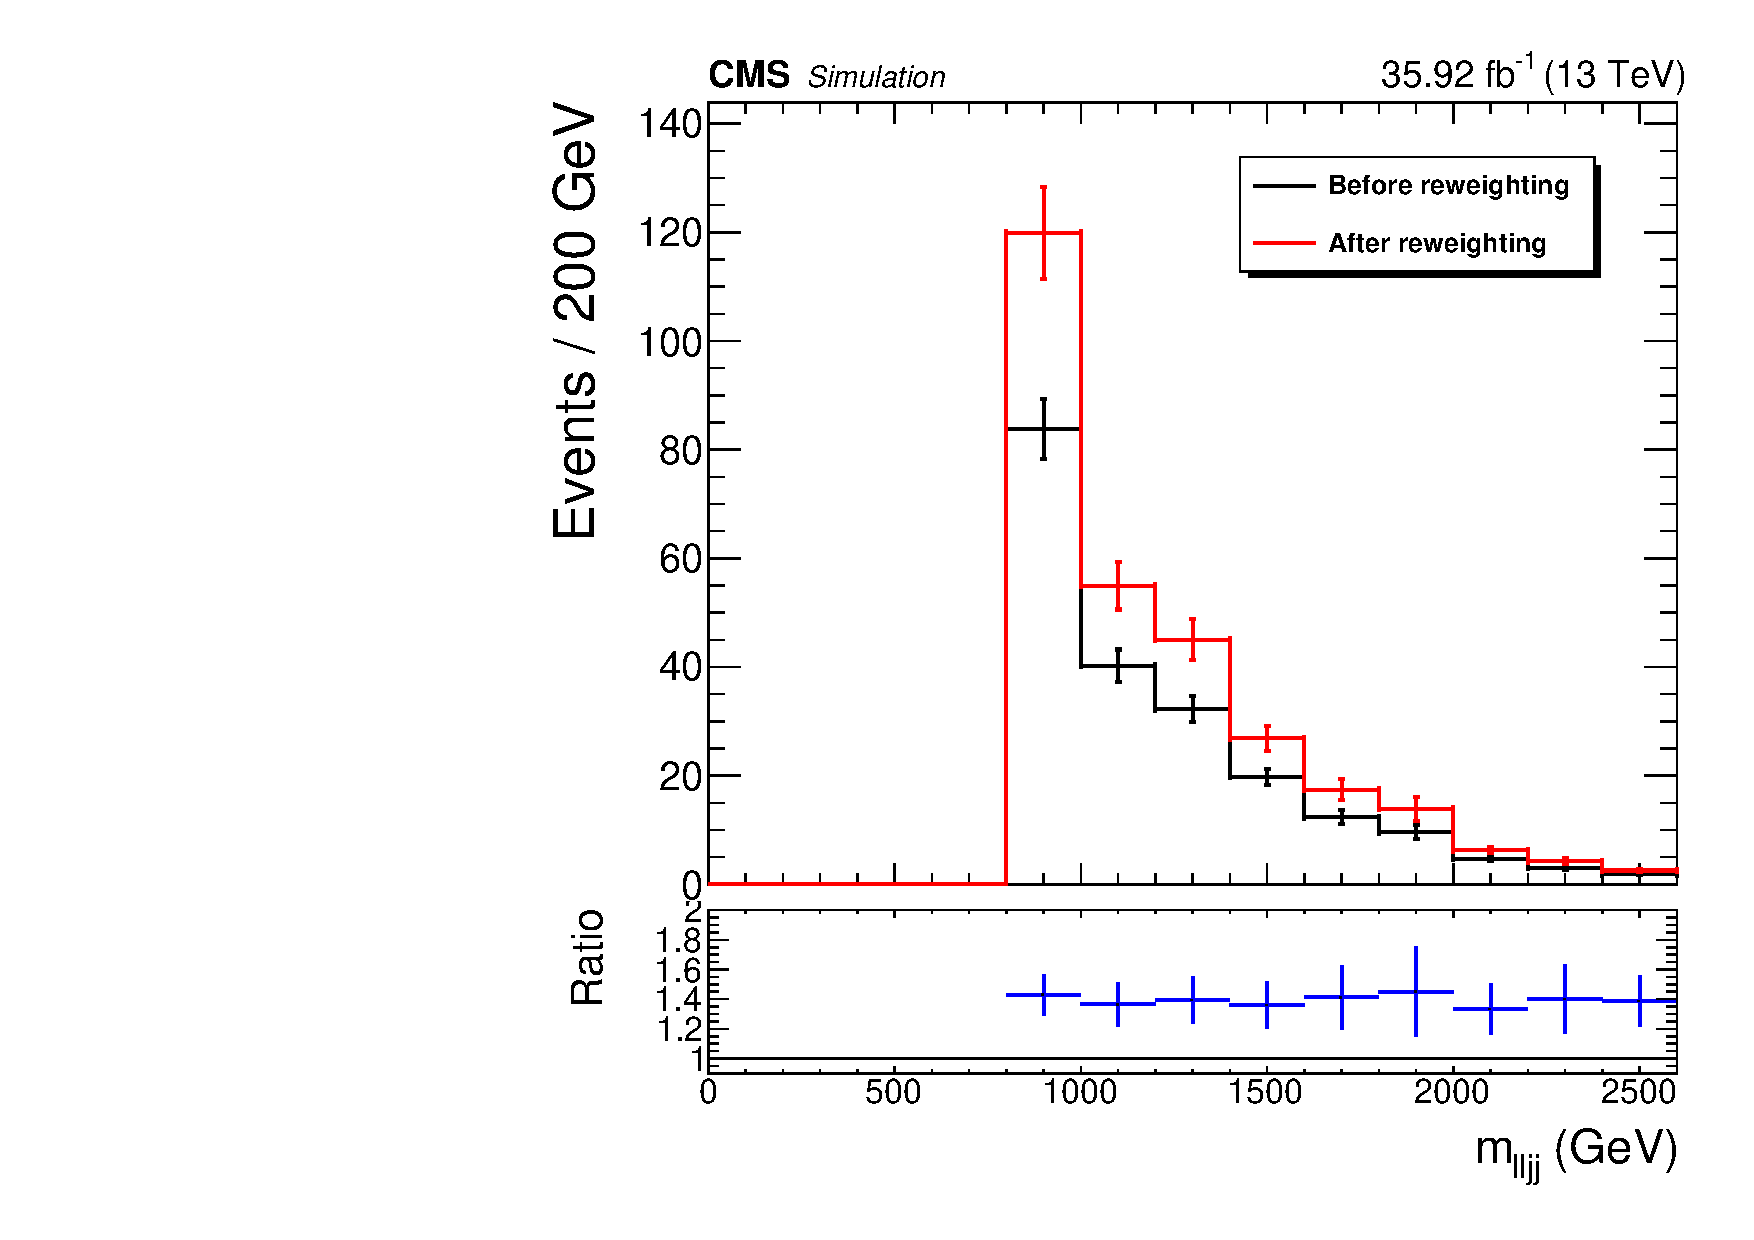
\includegraphics[width=0.45\textwidth]{figures/2016/Resolved_SR_Muon_WRCand_Mass.pdf}
  \vspace{0.01\textwidth}

  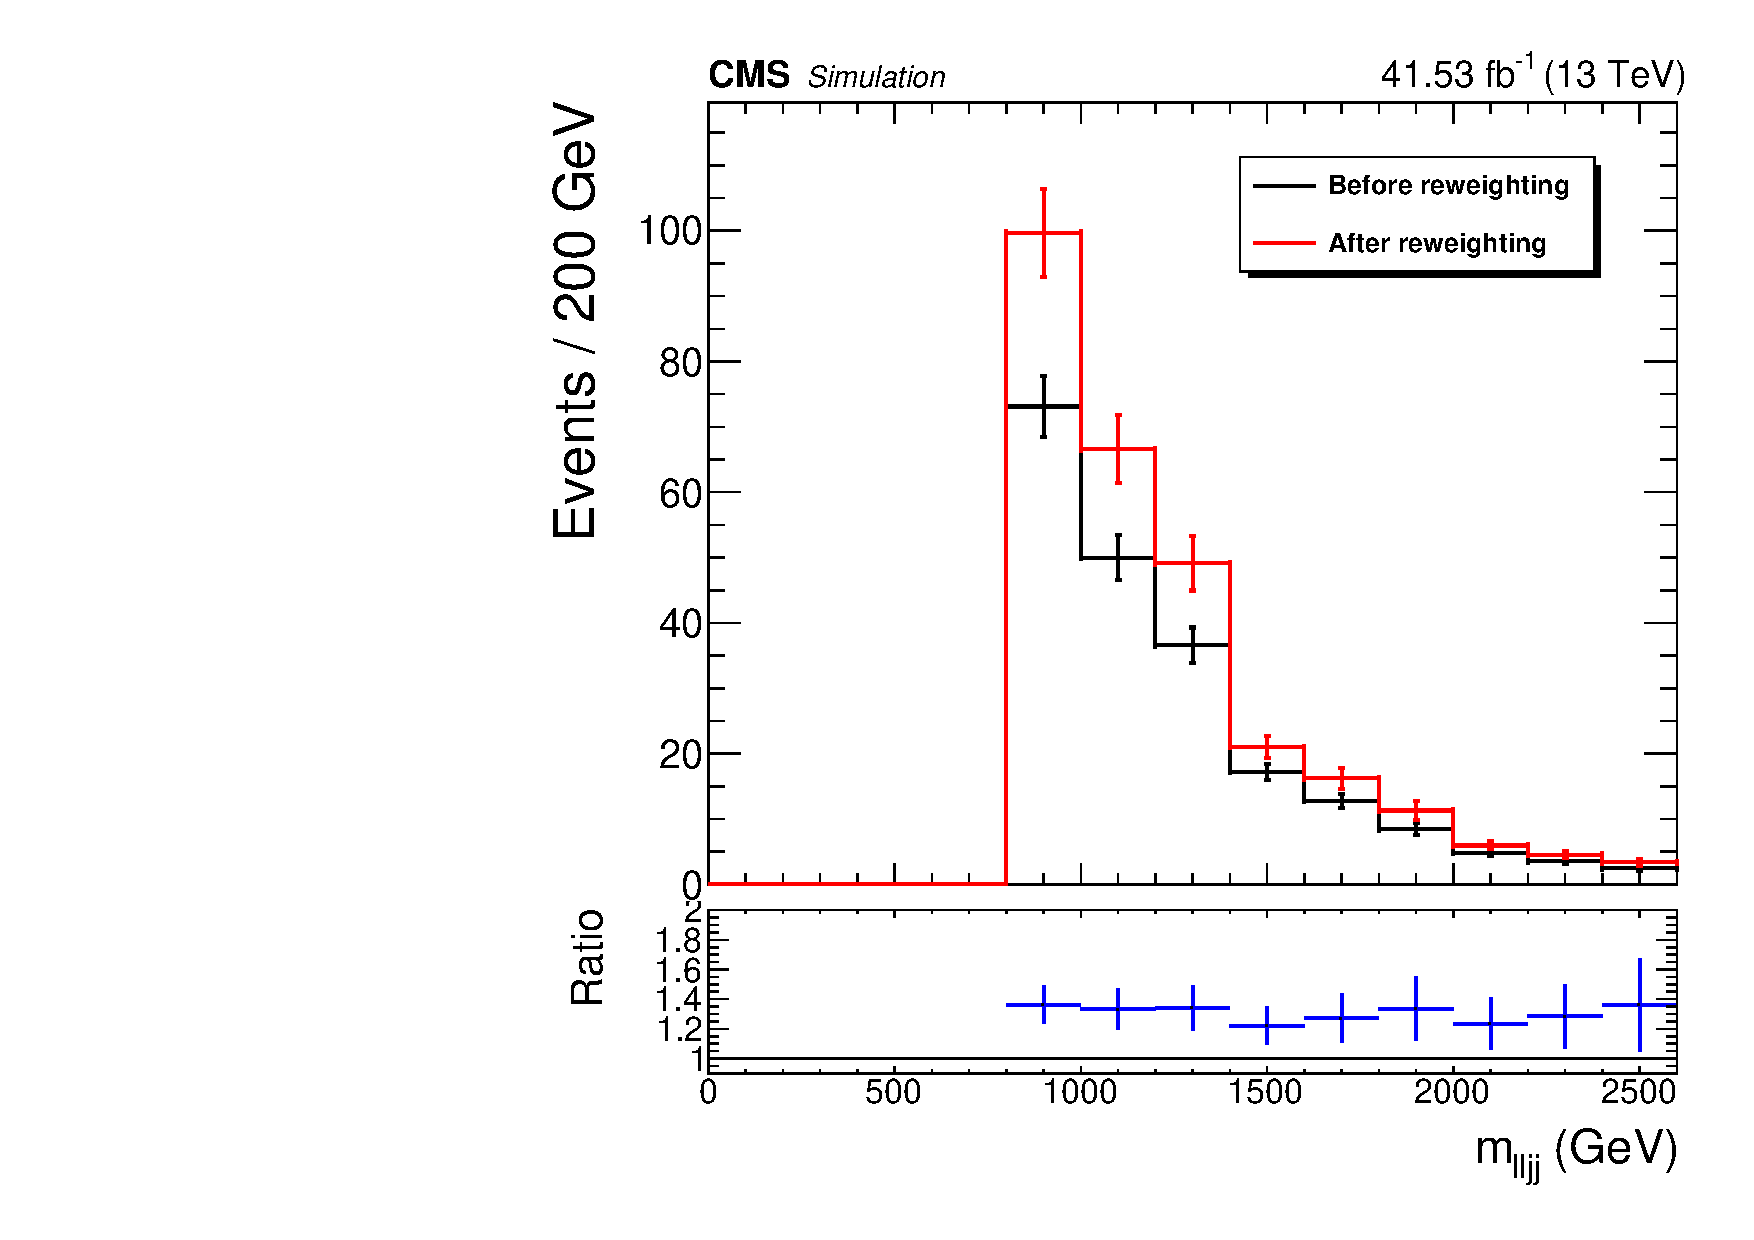
\includegraphics[width=0.45\textwidth]{figures/2017/Resolved_SR_Electron_WRCand_Mass.pdf}
  \hspace{0.01\textwidth}
  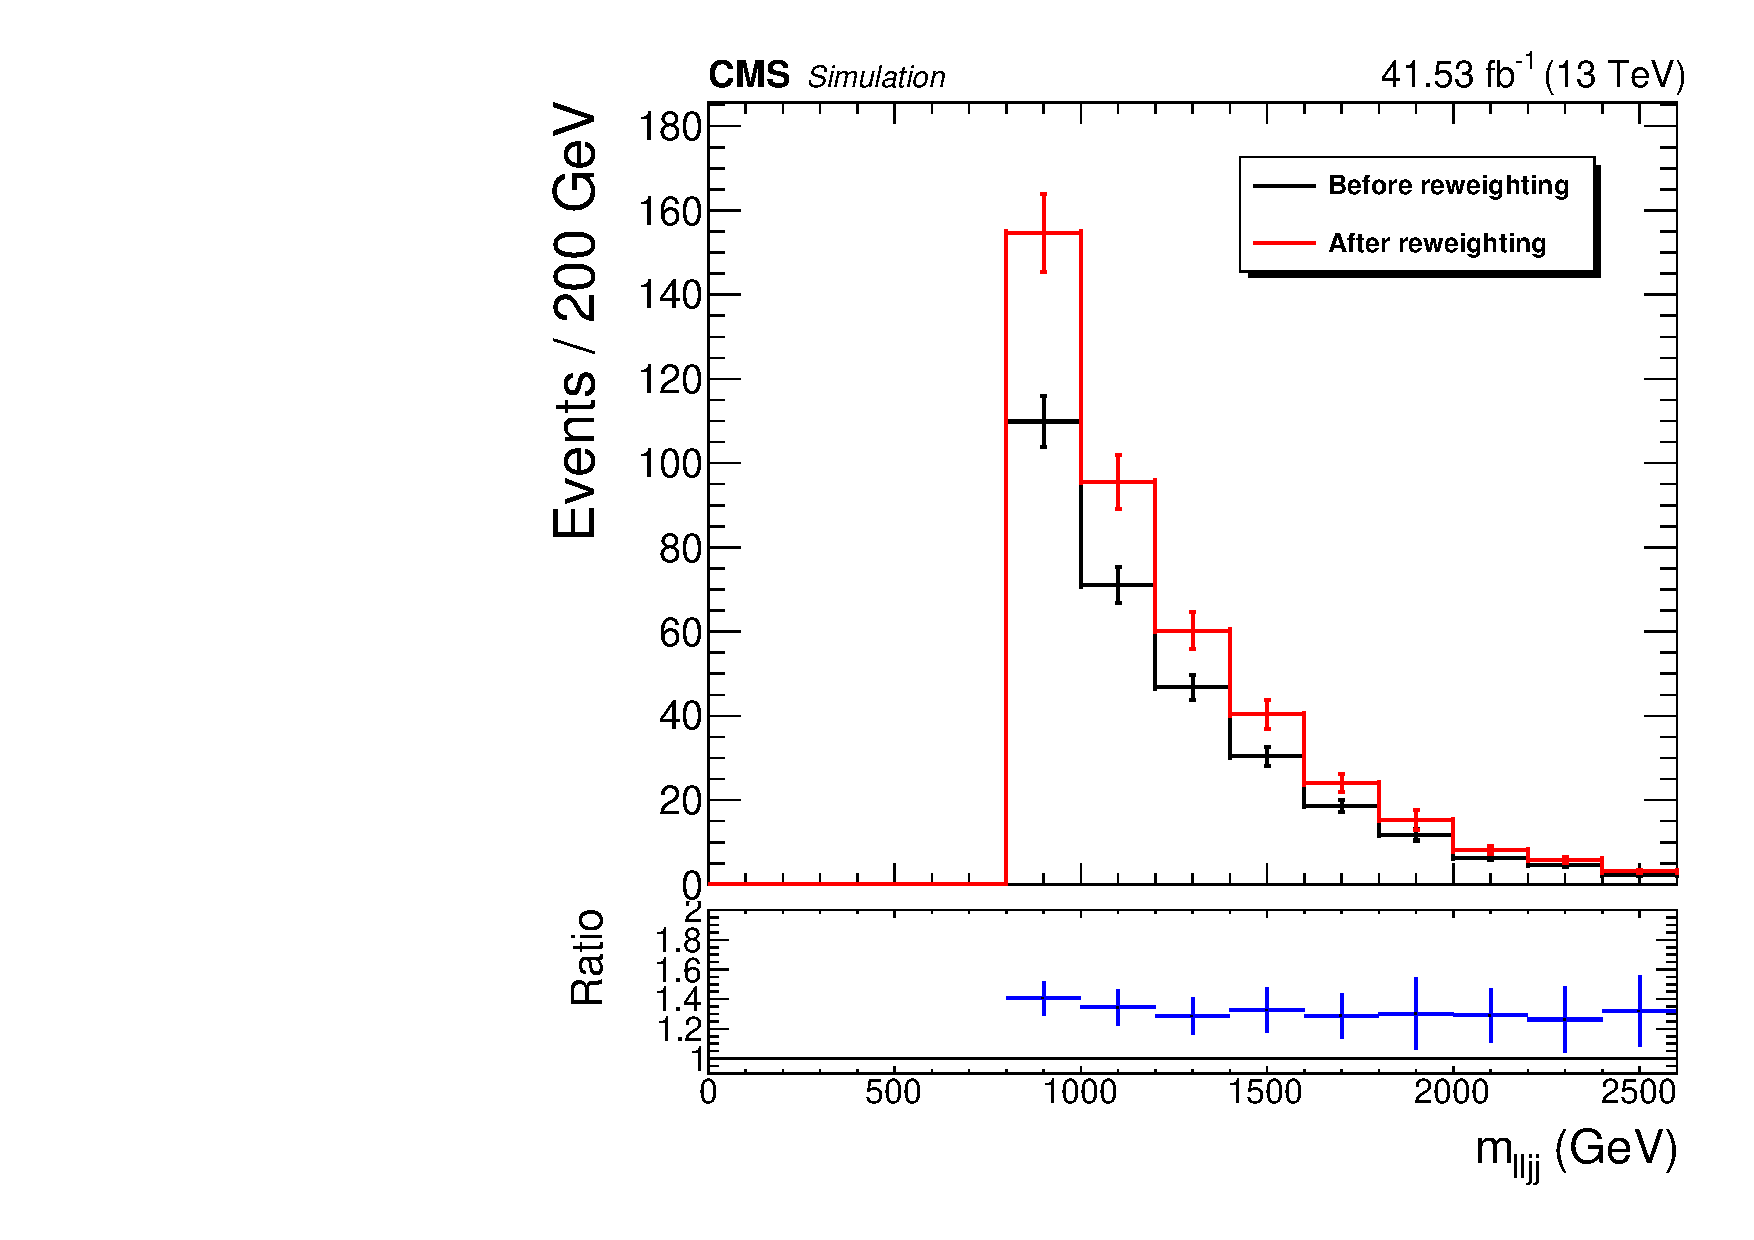
\includegraphics[width=0.45\textwidth]{figures/2017/Resolved_SR_Muon_WRCand_Mass.pdf}
  \vspace{0.01\textwidth}

  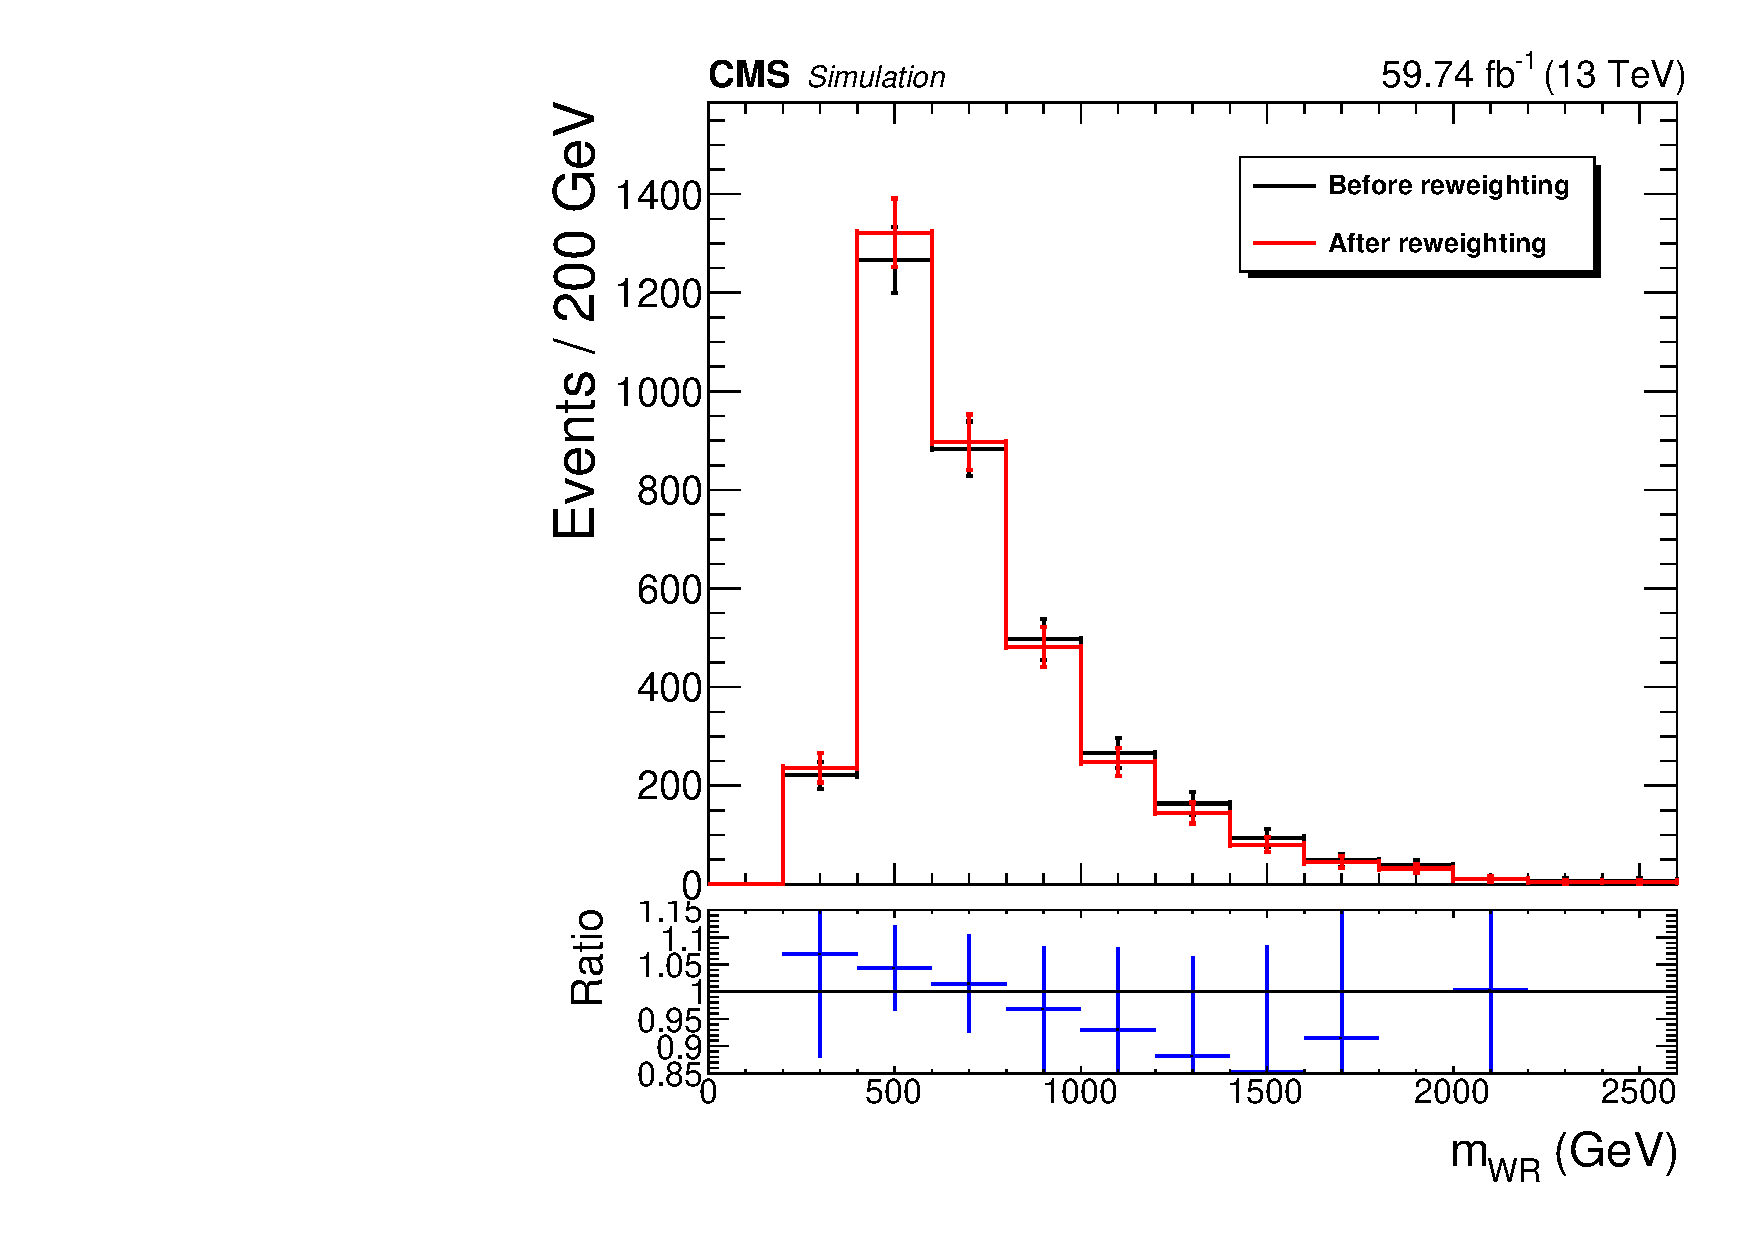
\includegraphics[width=0.45\textwidth]{figures/2018/Resolved_SR_Electron_WRCand_Mass.pdf}
  \hspace{0.01\textwidth}
  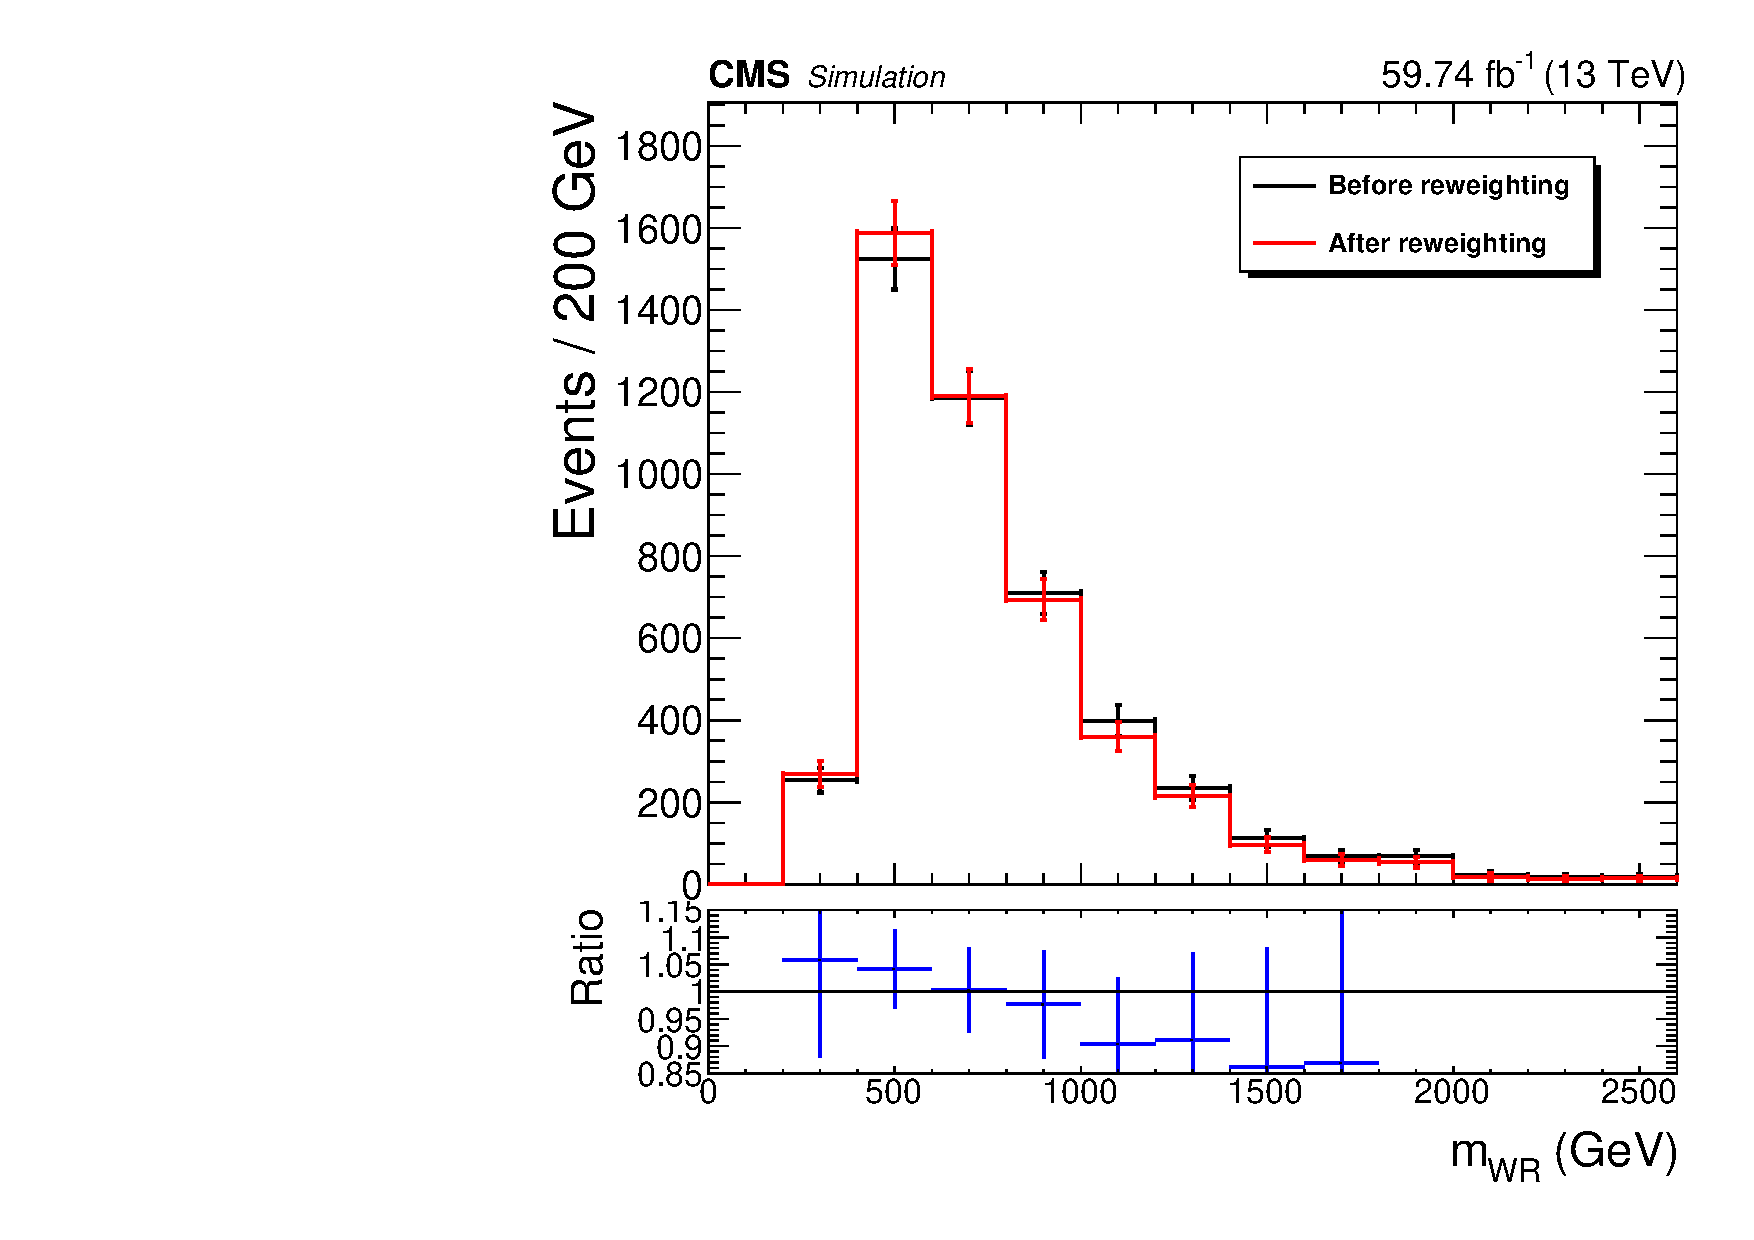
\includegraphics[width=0.45\textwidth]{figures/2018/Resolved_SR_Muon_WRCand_Mass.pdf}

  \topcaption{
    The reconstructed \PWR mass distributions in the resolved signal region, before and after applying $\PZ$-$\pt$ reweighting.
  }
  \label{fig:BkgdZptSRCompResolved}
\end{figure}

\begin{figure}[htbp]
  \centering

  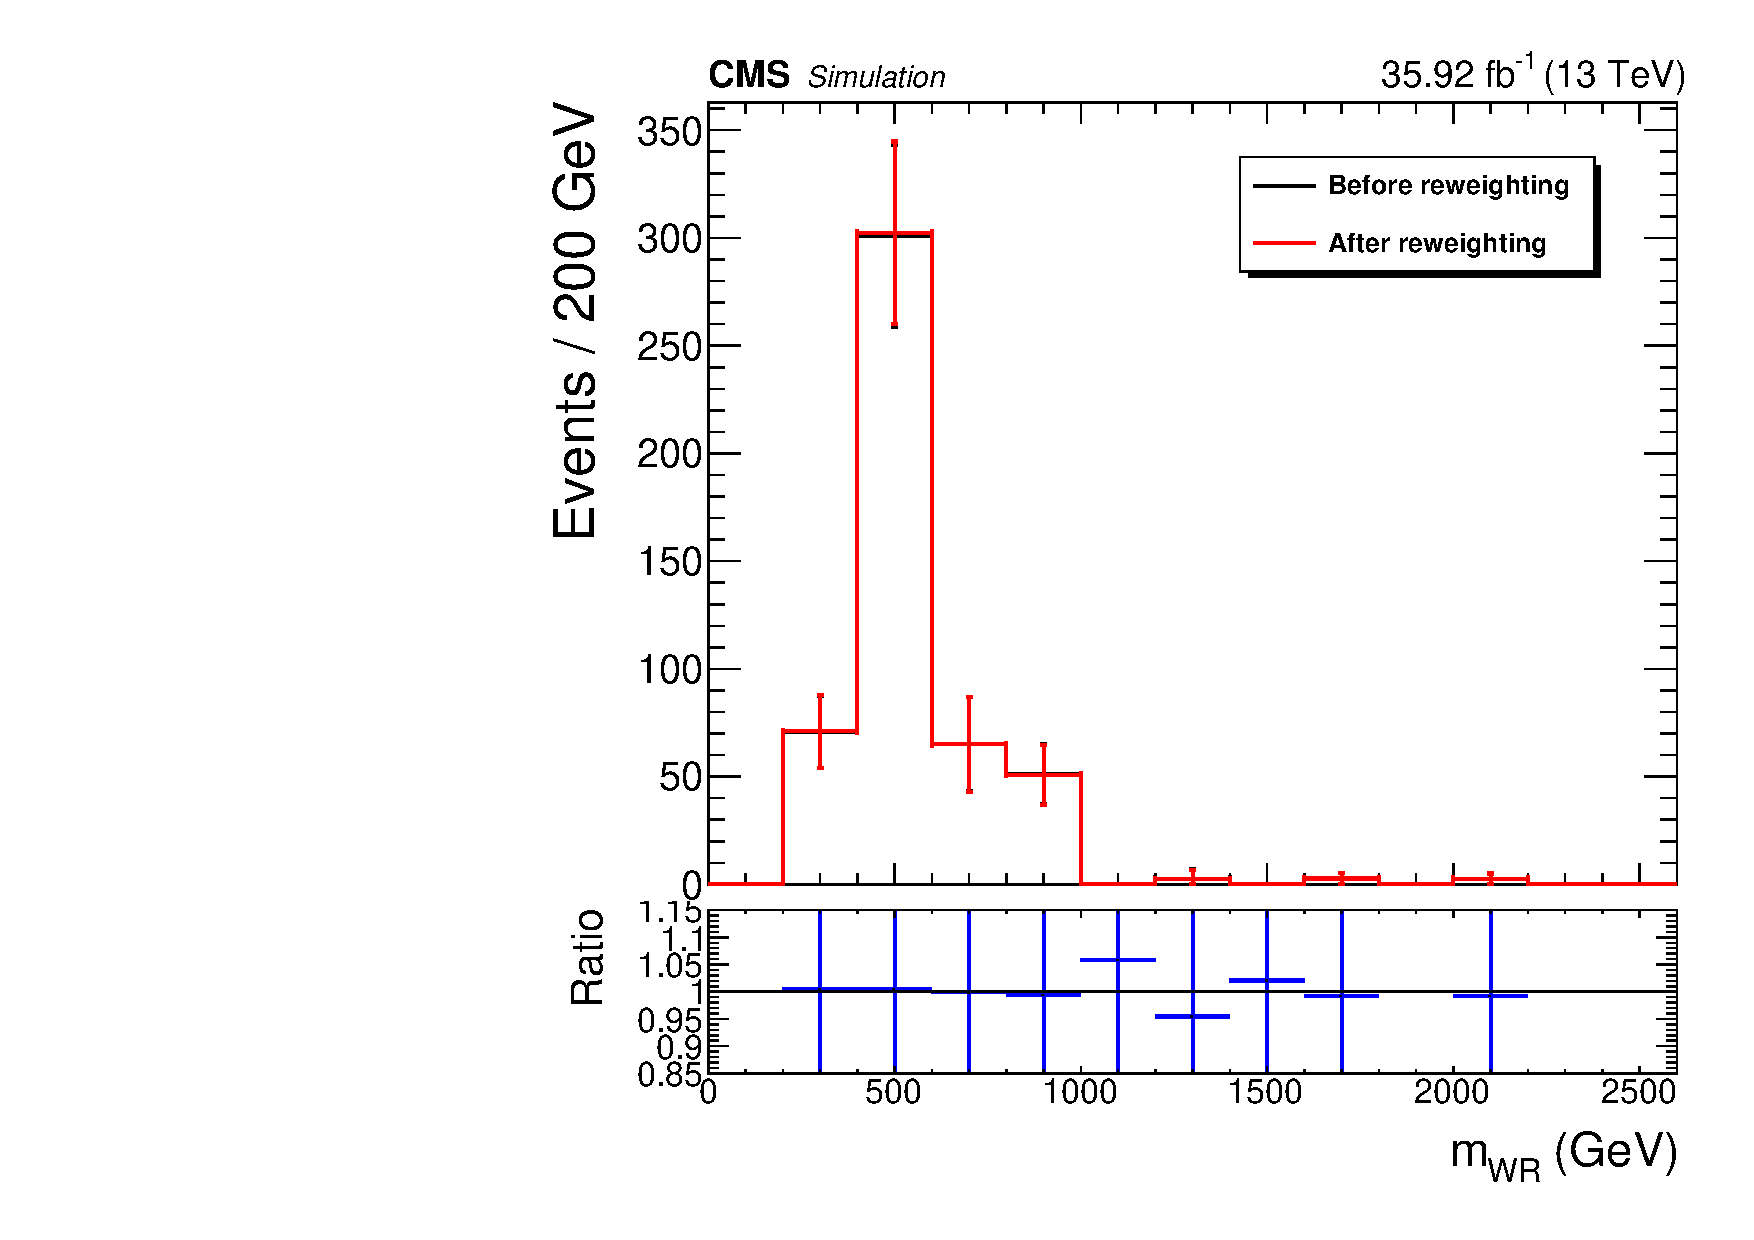
\includegraphics[width=0.45\textwidth]{figures/2016/Boosted_SR_Electron_WRCand_Mass.pdf}
  \hspace{0.01\textwidth}
  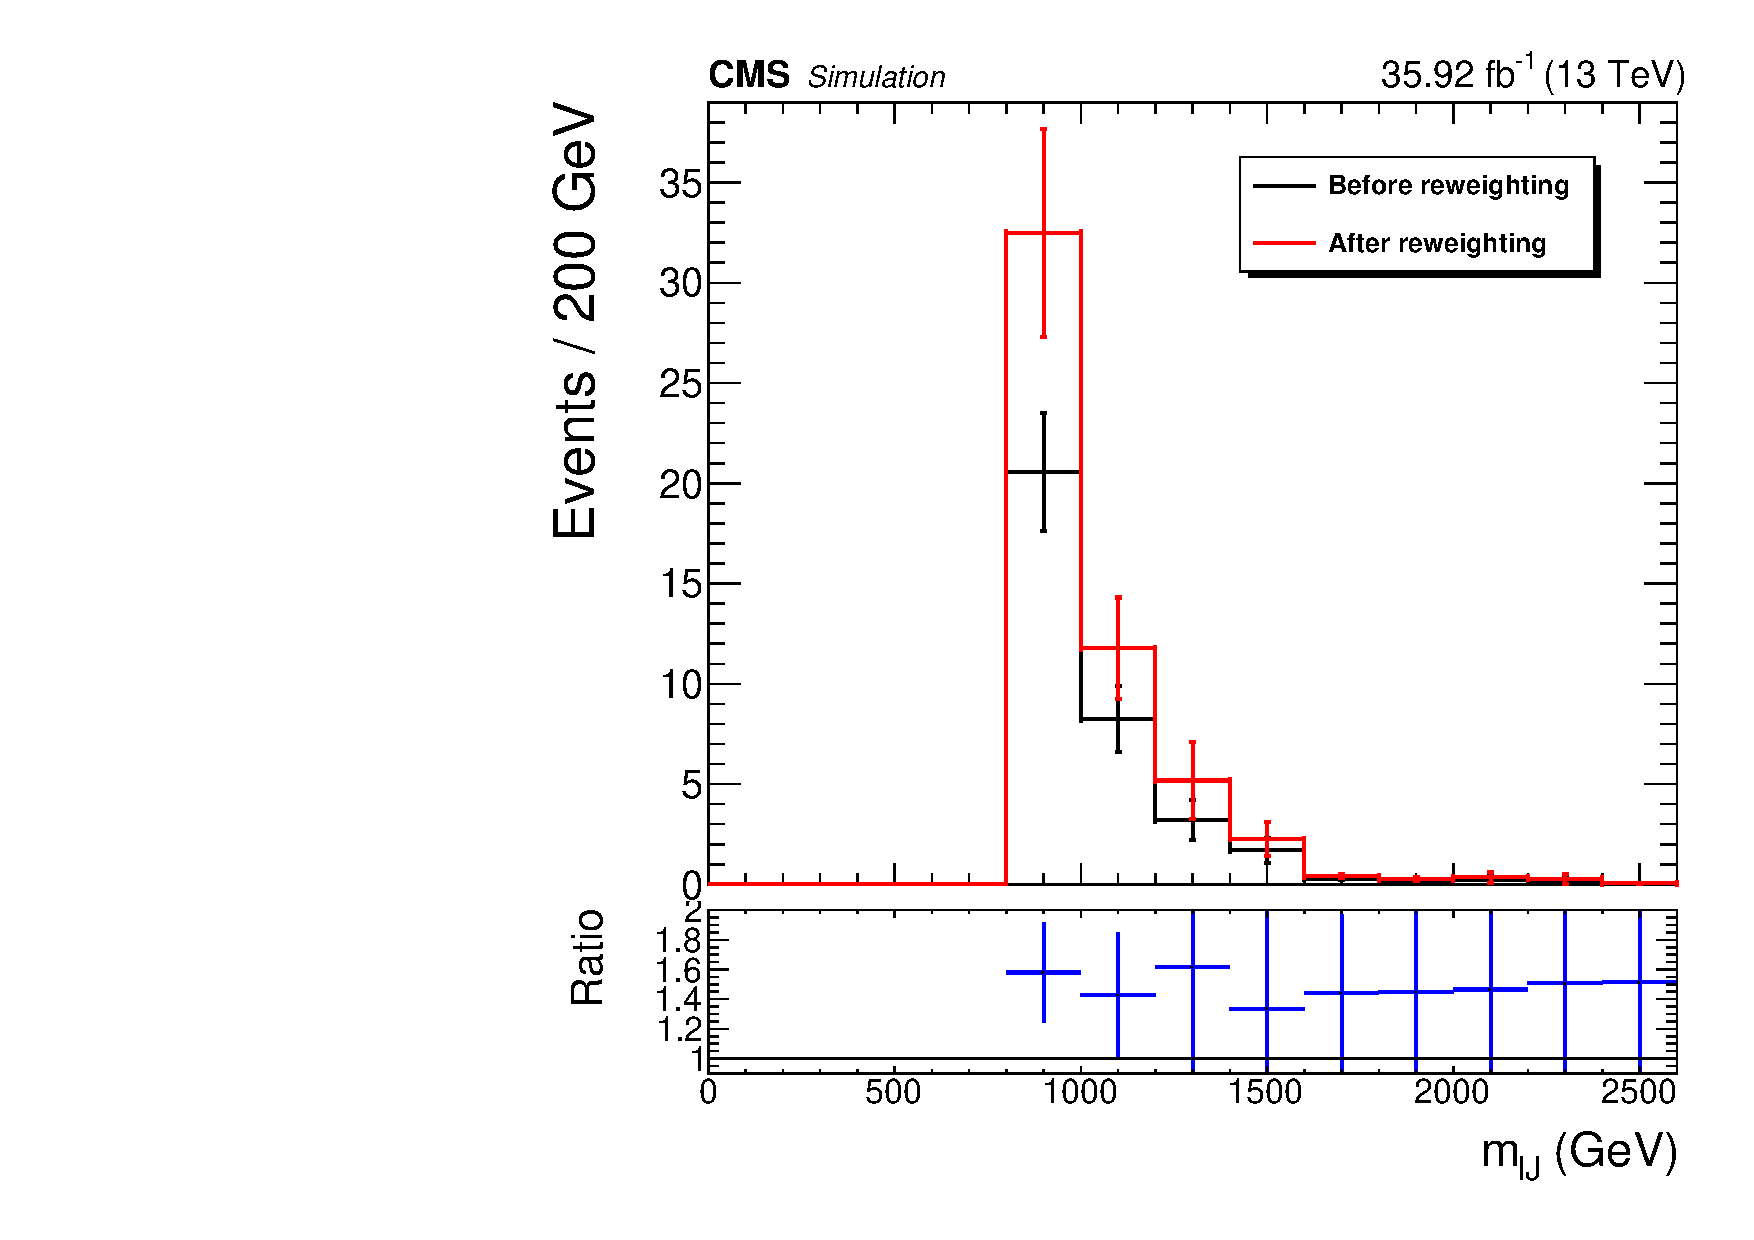
\includegraphics[width=0.45\textwidth]{figures/2016/Boosted_SR_Muon_WRCand_Mass.pdf}
  \vspace{0.01\textwidth}

  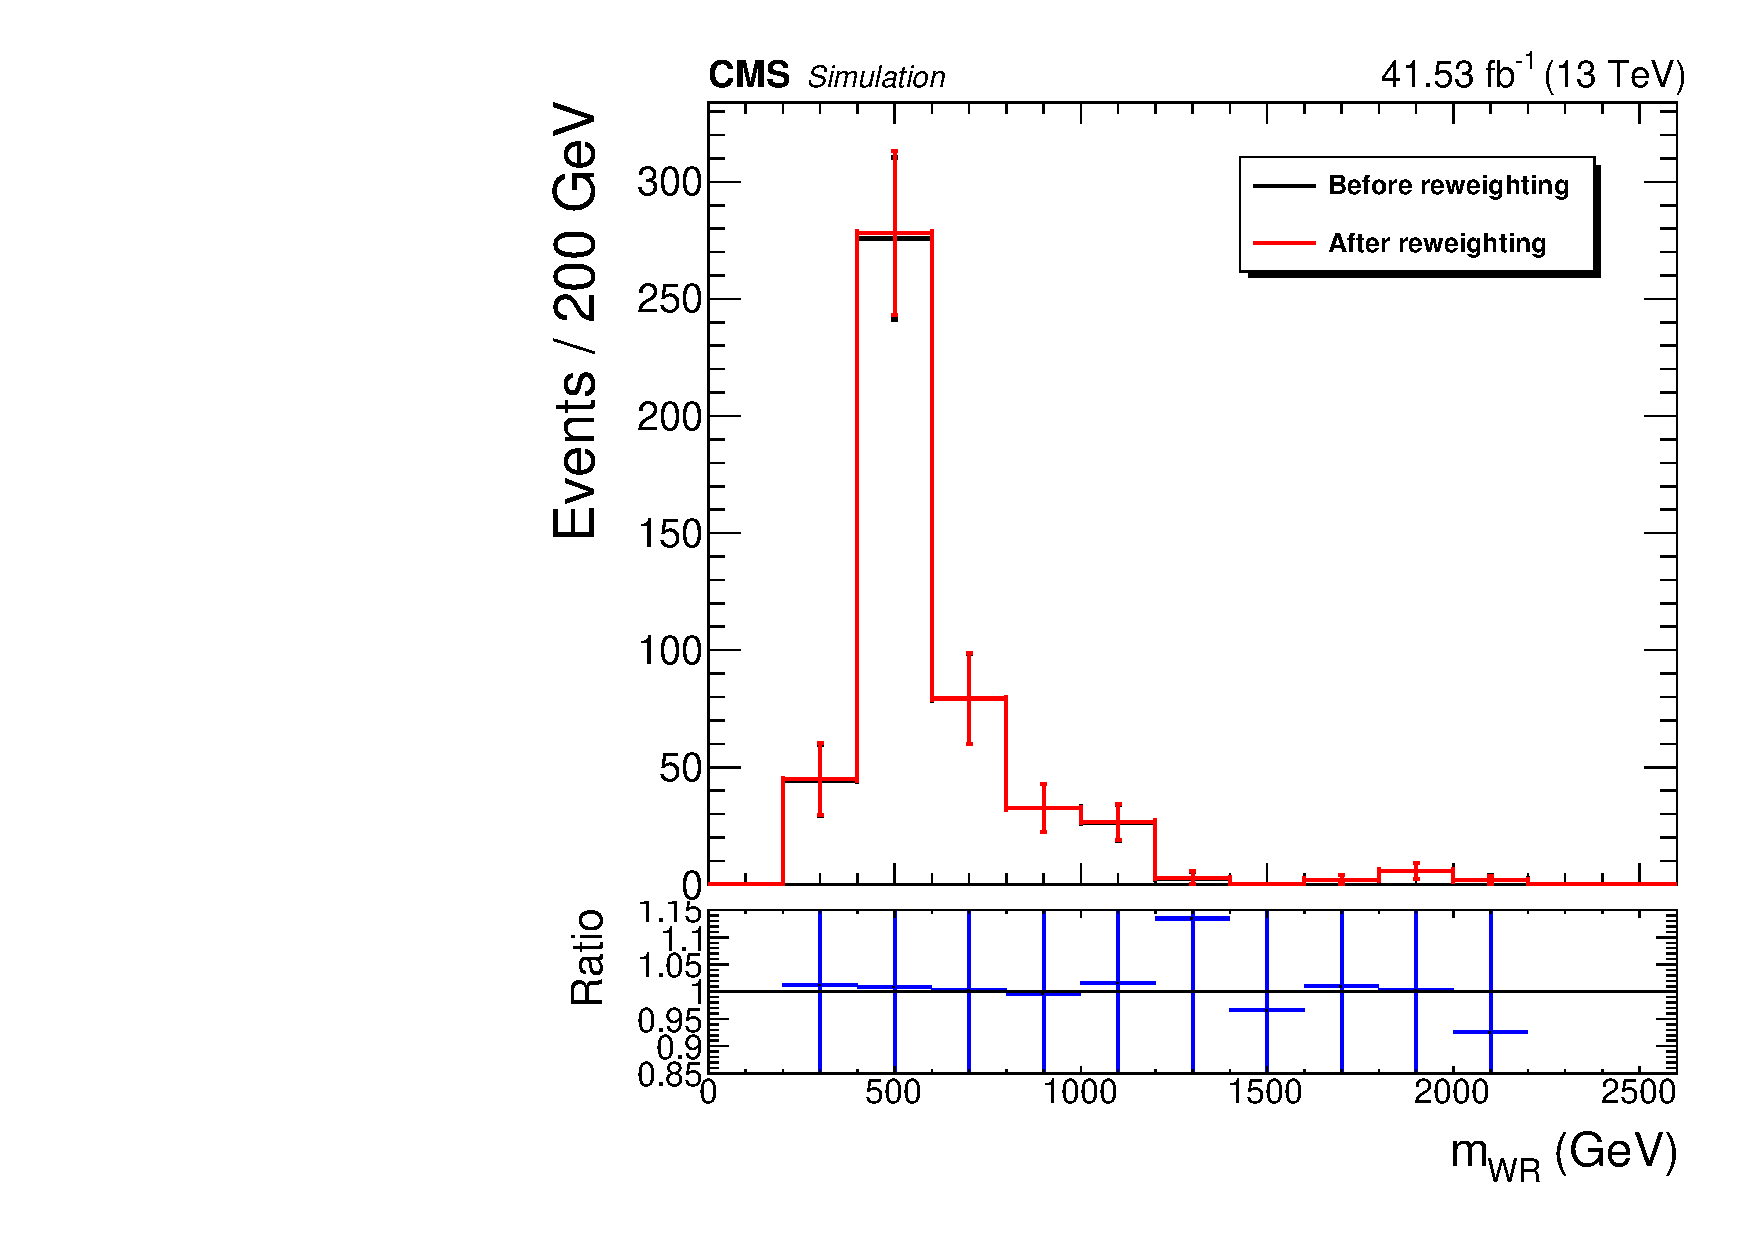
\includegraphics[width=0.45\textwidth]{figures/2017/Boosted_SR_Electron_WRCand_Mass.pdf}
  \hspace{0.01\textwidth}
  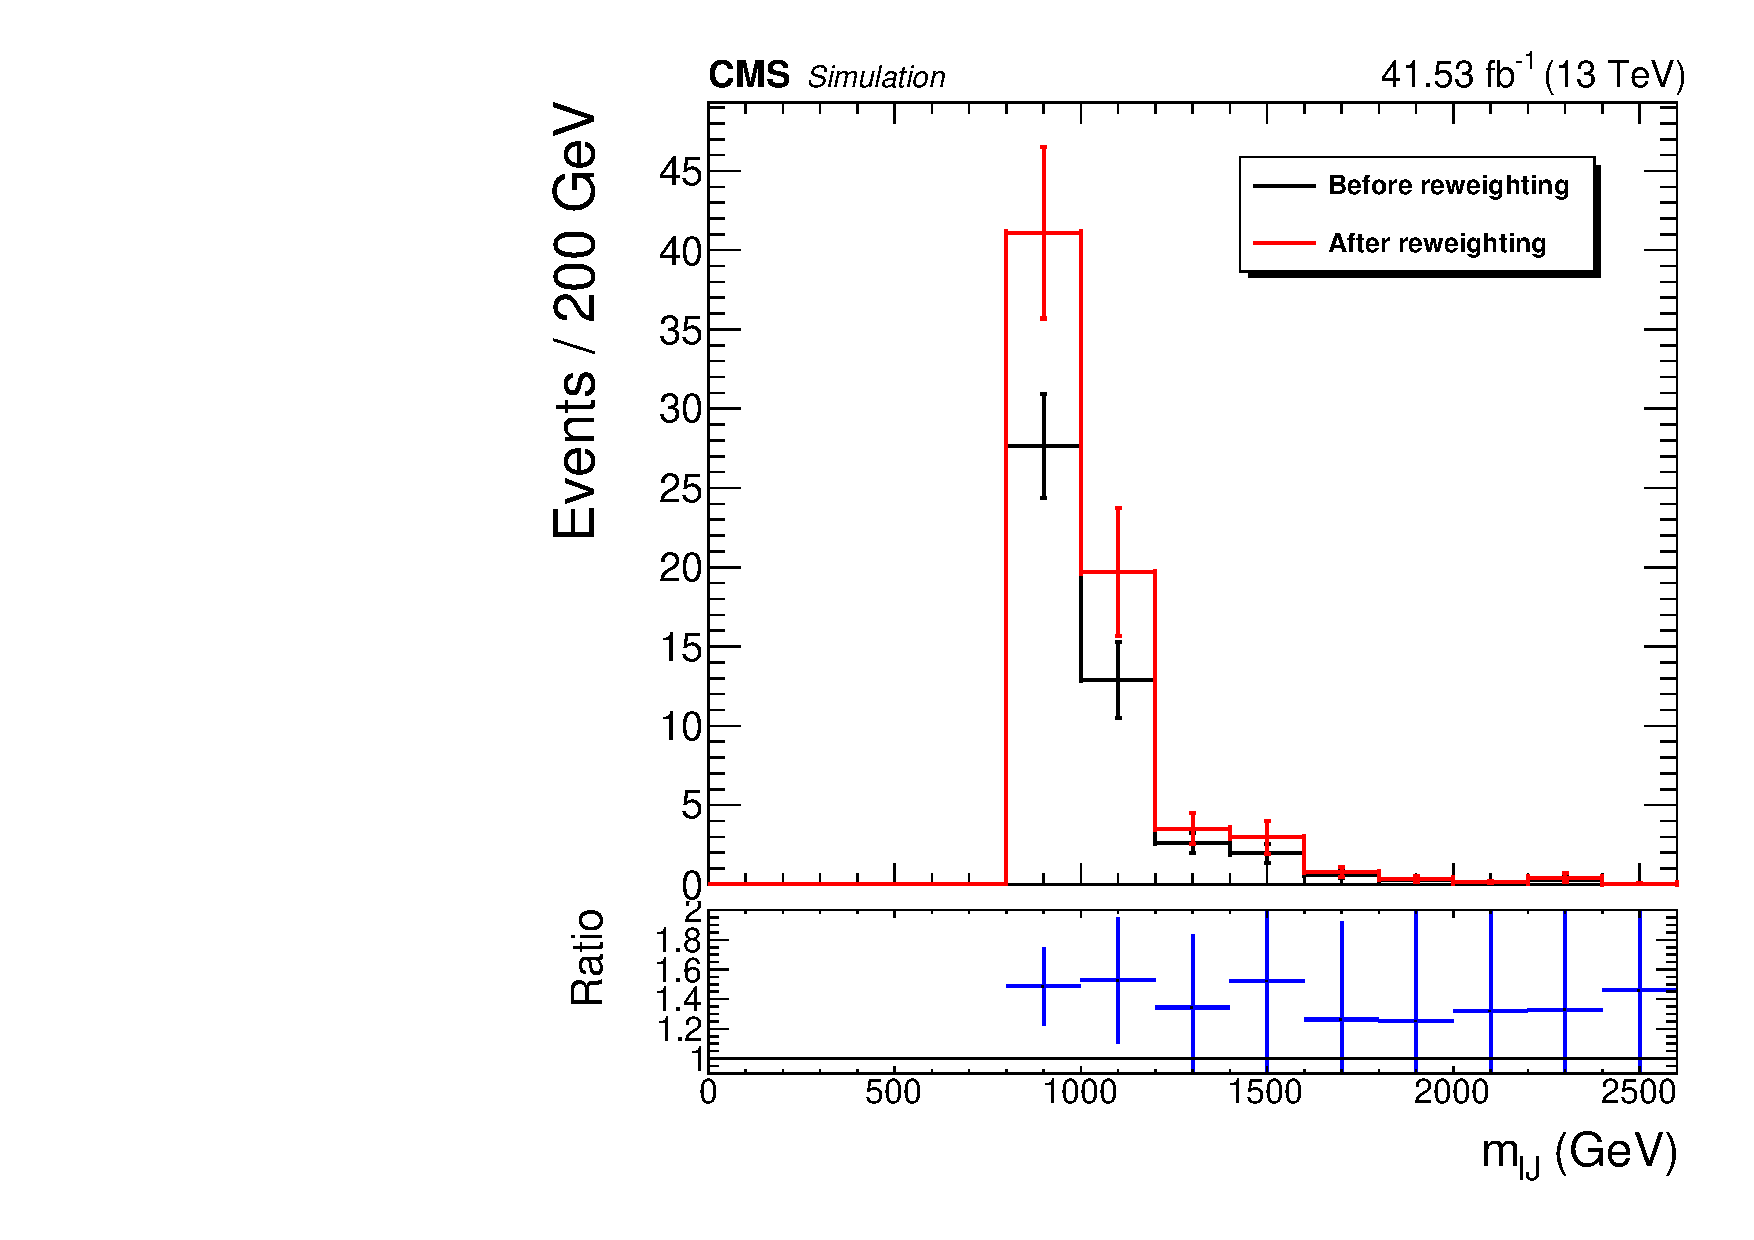
\includegraphics[width=0.45\textwidth]{figures/2017/Boosted_SR_Muon_WRCand_Mass.pdf}
  \vspace{0.01\textwidth}

  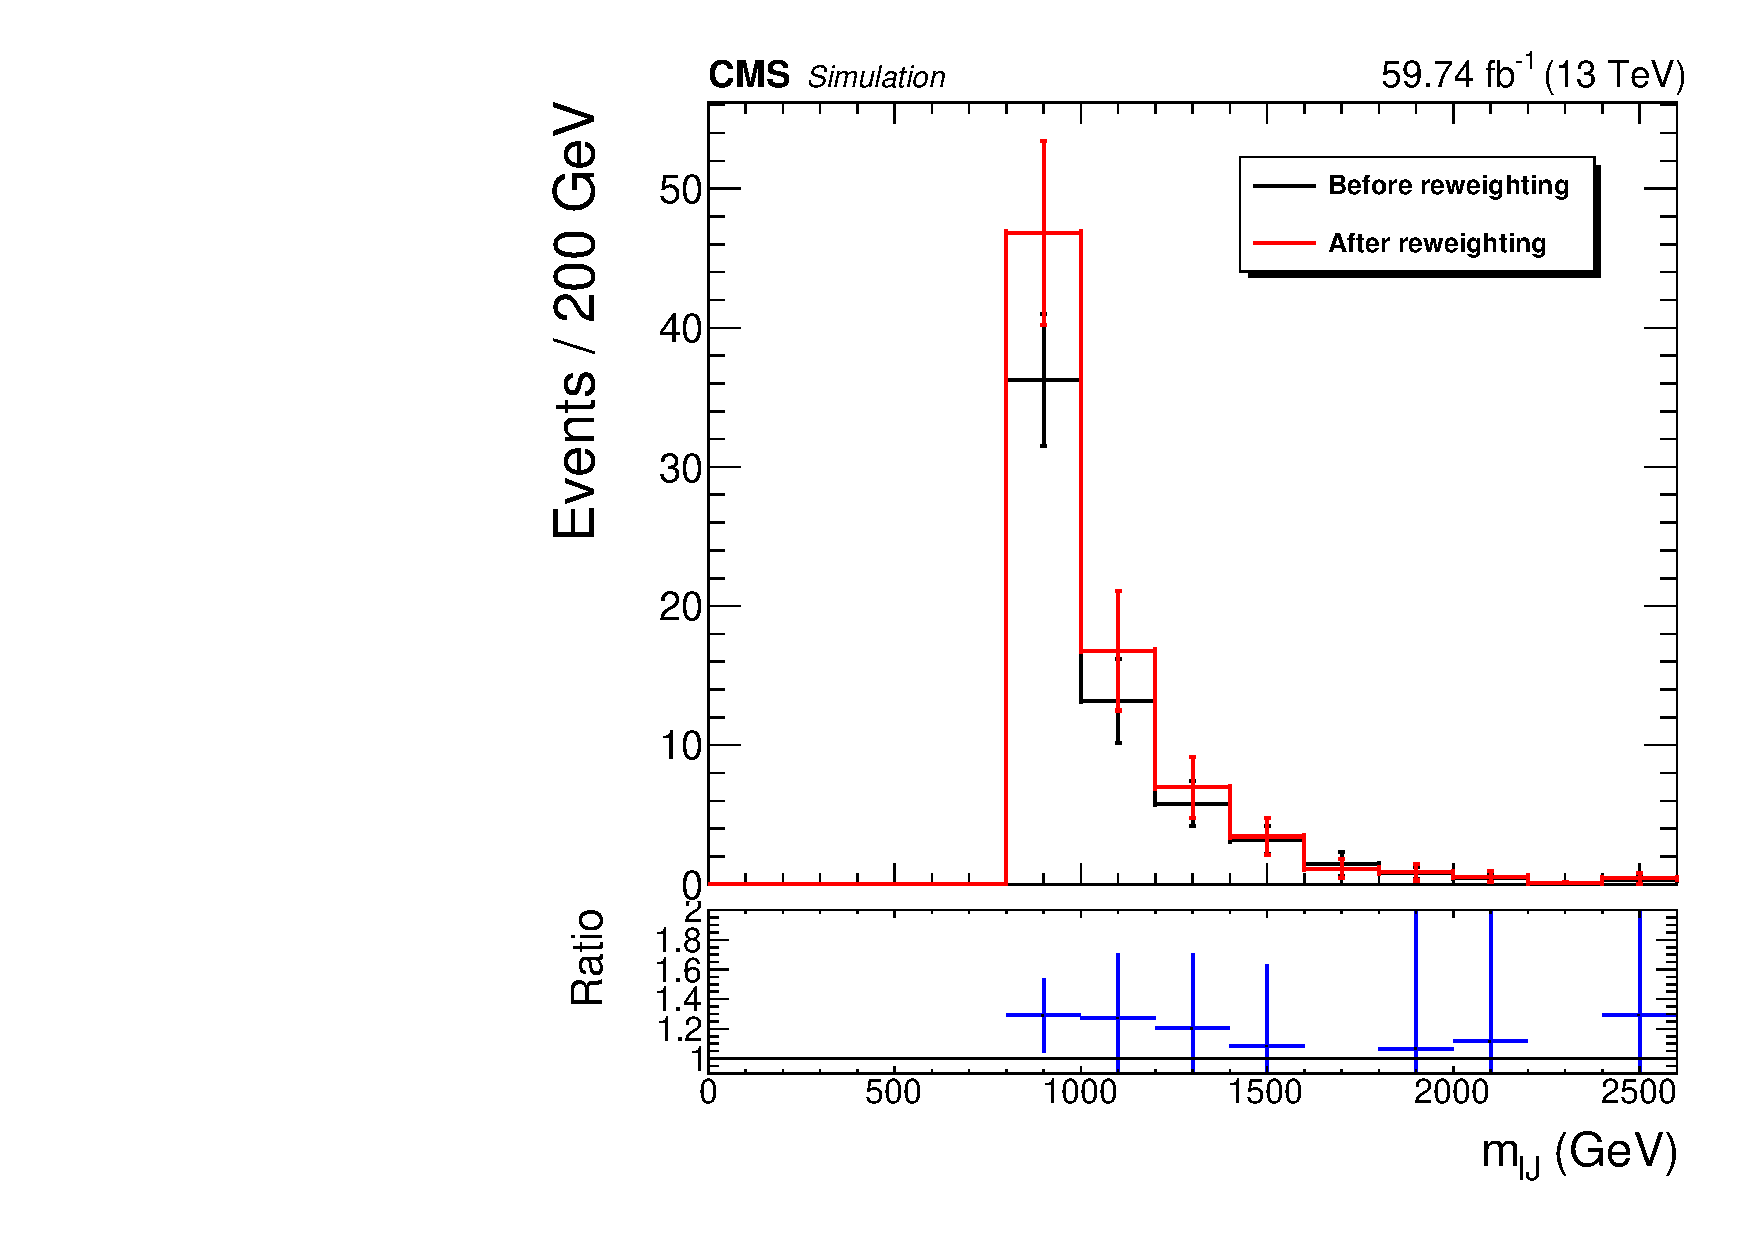
\includegraphics[width=0.45\textwidth]{figures/2018/Boosted_SR_Electron_WRCand_Mass.pdf}
  \hspace{0.01\textwidth}
  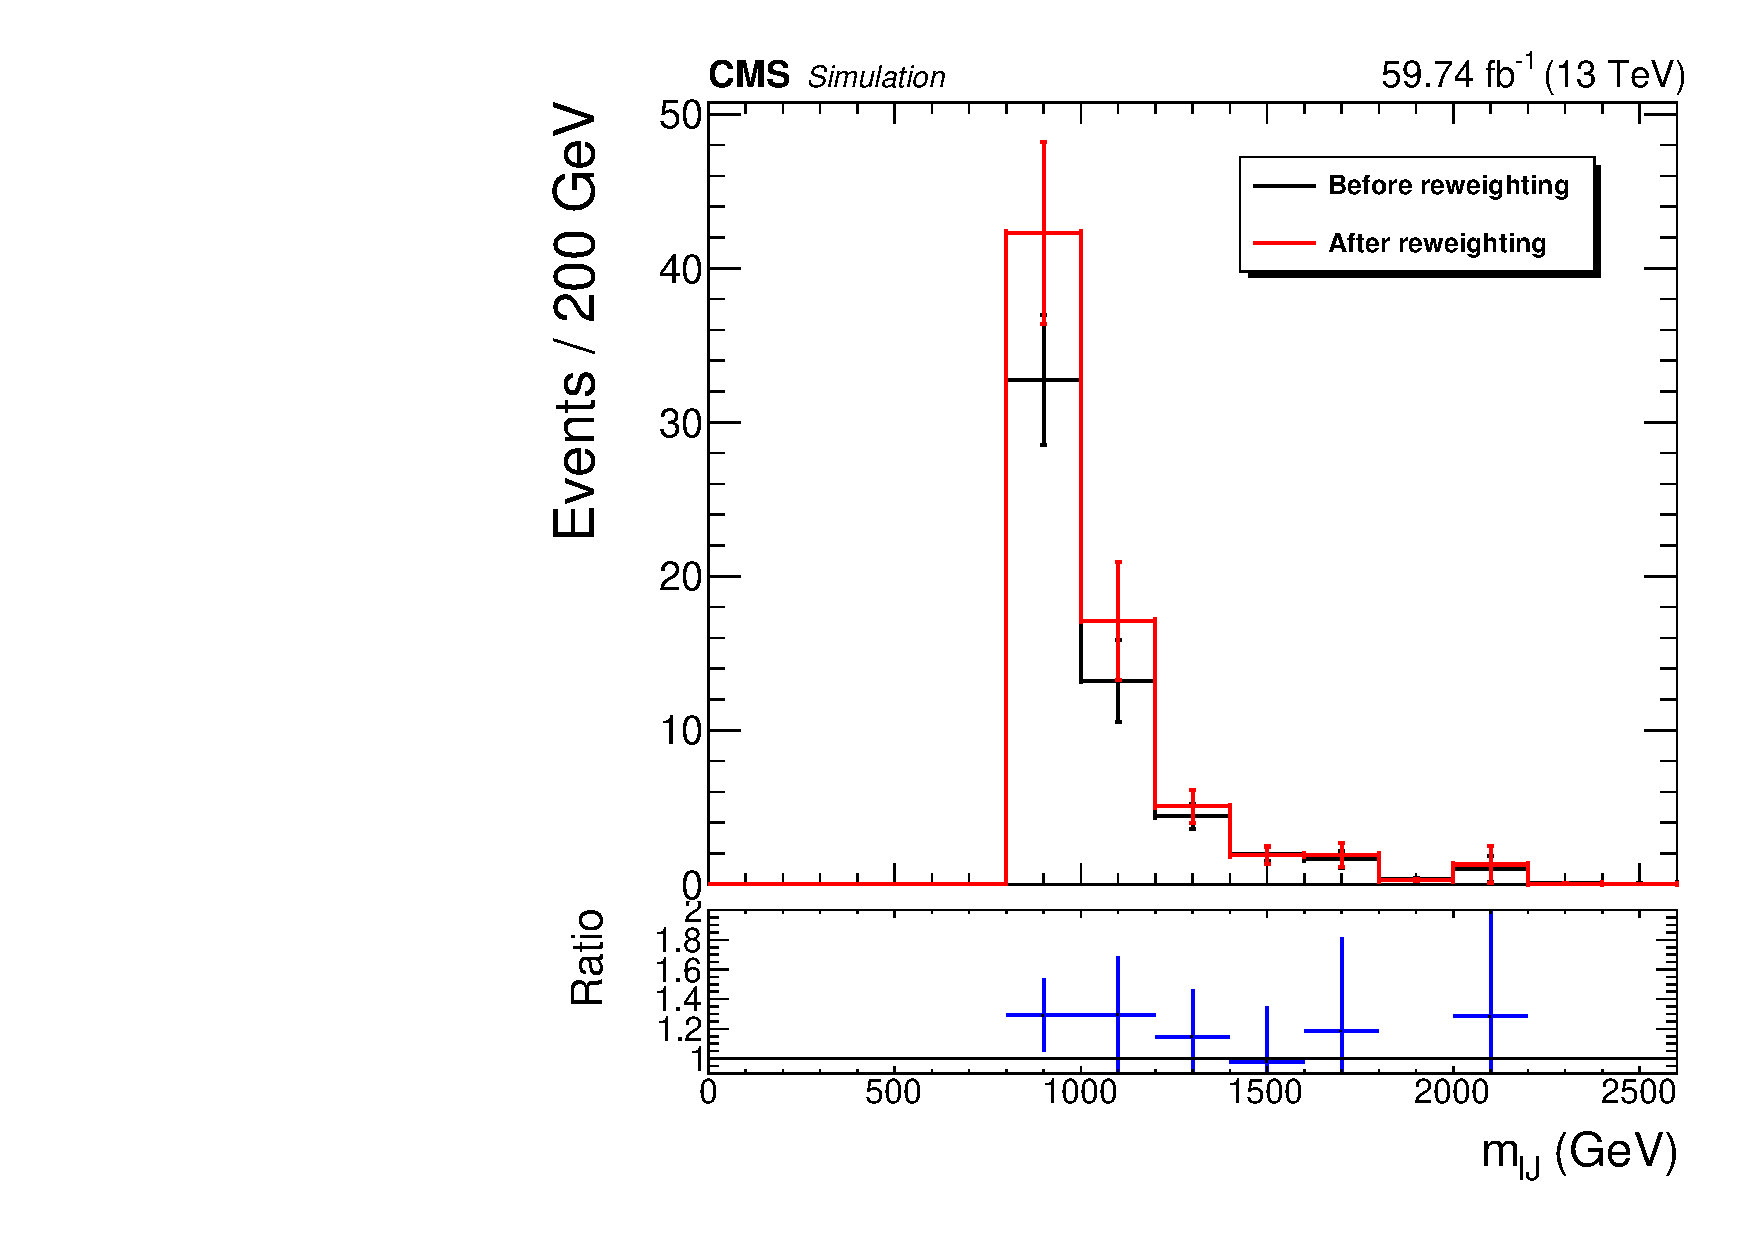
\includegraphics[width=0.45\textwidth]{figures/2018/Boosted_SR_Muon_WRCand_Mass.pdf}

  \topcaption{
    The reconstructed \PWR mass distributions in the boosted signal region, before and after applying $\PZ$-$\pt$ reweighting.
  }
  \label{fig:BkgdZptSRCompBoosted}
\end{figure}



\subsubsection{Resolved}
\iffalse
The invariant mass distributions in the resolved low $m_{ll}$ control region are shown in Figure~\ref{fig:ResZPeak} for all three years of data taking.

\begin{figure}[h!]\begin{center}
    \includegraphics[width=0.49\textwidth]{figures/2016/resolvedRECOmass_ZPeak.png}
    \includegraphics[width=0.49\textwidth]{figures/2017/resolvedRECOmass_ZPeak.png}\\
    \includegraphics[width=0.49\textwidth]{figures/2018/resolvedRECOmass_ZPeak.png}
    \caption{The 4-object invariant mass distribution in the resolved low $m_{ll}$ control region in 2016 (top left), 2017 (top right), and 2018 (bottom).}
 \label{fig:ResZPeak}
 \end{center}
 \end{figure}
\fi
{\color{red} TO DO SF results for each year}

\subsubsection{Boosted}
\iffalse
The invariant mass distributions in the boosted low $m_{ll}$ control region are shown in Figure~\ref{fig:ResZPeak} for all three years of data taking.

\begin{figure}[h!]\begin{center}
    \includegraphics[width=0.49\textwidth]{figures/2016/leadAK8JetMuonMass_noLSF.png}
    \includegraphics[width=0.49\textwidth]{figures/2017/leadAK8JetMuonMass_noLSF.png}\\
    \includegraphics[width=0.49\textwidth]{figures/2018/leadAK8JetMuonMass_noLSF.png}
    \caption{The 2-object invariant mass distribution in the boosted low $m_{ll}$ control region in 2016 (top left), 2017 (top right), and 2018 (bottom).}
 \label{fig:BoostZPeak}
 \end{center}
 \end{figure}
\fi
{\color{red} TO DO SF results for each year}

\subsection{ttbar+Jets background estimation}
\label{sec:ttbarBkgd}
The \ttbar background contribution is estimated from simulation while a correction factor is derived in the flavor sideband CR, which has the same kinematics as the \ttbar in the signal region.
The contribution from other backgrounds in this CR is taken from simulation and subtracted from the data to produce a pure \ttbar sample.

For this estimate, the assumption made on the conservation of the flavor in the decay is needed to ensure that there is no contamination from signal events.
Thus, the decay of a real $\PWR$ boson at leading order cannot yield a $\Pe\mu$ final state and the flavor sideband is dominated by $\ttbar$ events.

To calculate the number of events from $\ttbar$ in the dimuon signal region, for both the boosted and resolved analyses, we used the $\ttbar$ MC to find the SFs $R_{\Pe\mu/\mu\mu}$ between the flavor sideband and the signal regions.
These SFs were evaluated from the ratio of the number of events in the final-state objects invariant mass distributions in the signal region over the invariant mass distribution in the flavor sideband.
The number of events in the signal region is given by:

\begin{equation}
N_{\ttbar}(\text{signal region}) = N_{\ttbar}(\text{flavor sideband})\times R_{\Pe\mu/\ell\ell}
\end{equation}

Using the SFs we can account for the difference in efficiency and acceptance between electrons and muons in these final states.

The ratios between the signal region and the $\Pe\mu$--sideband are obtained using \ttbar MC samples,
which are shown in Figs.~\ref{fig:emuRatioResolved}--\ref{fig:emuRatioBoosted}.
We fit the ratios with a contatant polynomial function, and the fit results are summarized in Table~\ref{tab:EMuRatioFit}.
\textcolor{red}{A preliminary systematic uncertainty $20~\%$ is assigned, which is enough to cover the ratio in whole $m_{\PWR}$ range.}

The $m(\PWR)$ distributions in the $\Pe\mu$--sideband are shown in Figs.~\ref{fig:emuDATAMCResolved}--\ref{fig:emuDATAMCBoosted}.
\textcolor{red}{For 2018 data analysis, $\PW$+Jets MC is not yet processed, which have considerable contributions in the boosted sideband events.}.

The comparison between the MC and data--driven method are shown in Figs.~\ref{fig:emuMCEMuCompResolved}--\ref{fig:emuMCEMuCompBoosted}.

\begin{figure}[htbp]
  \centering

  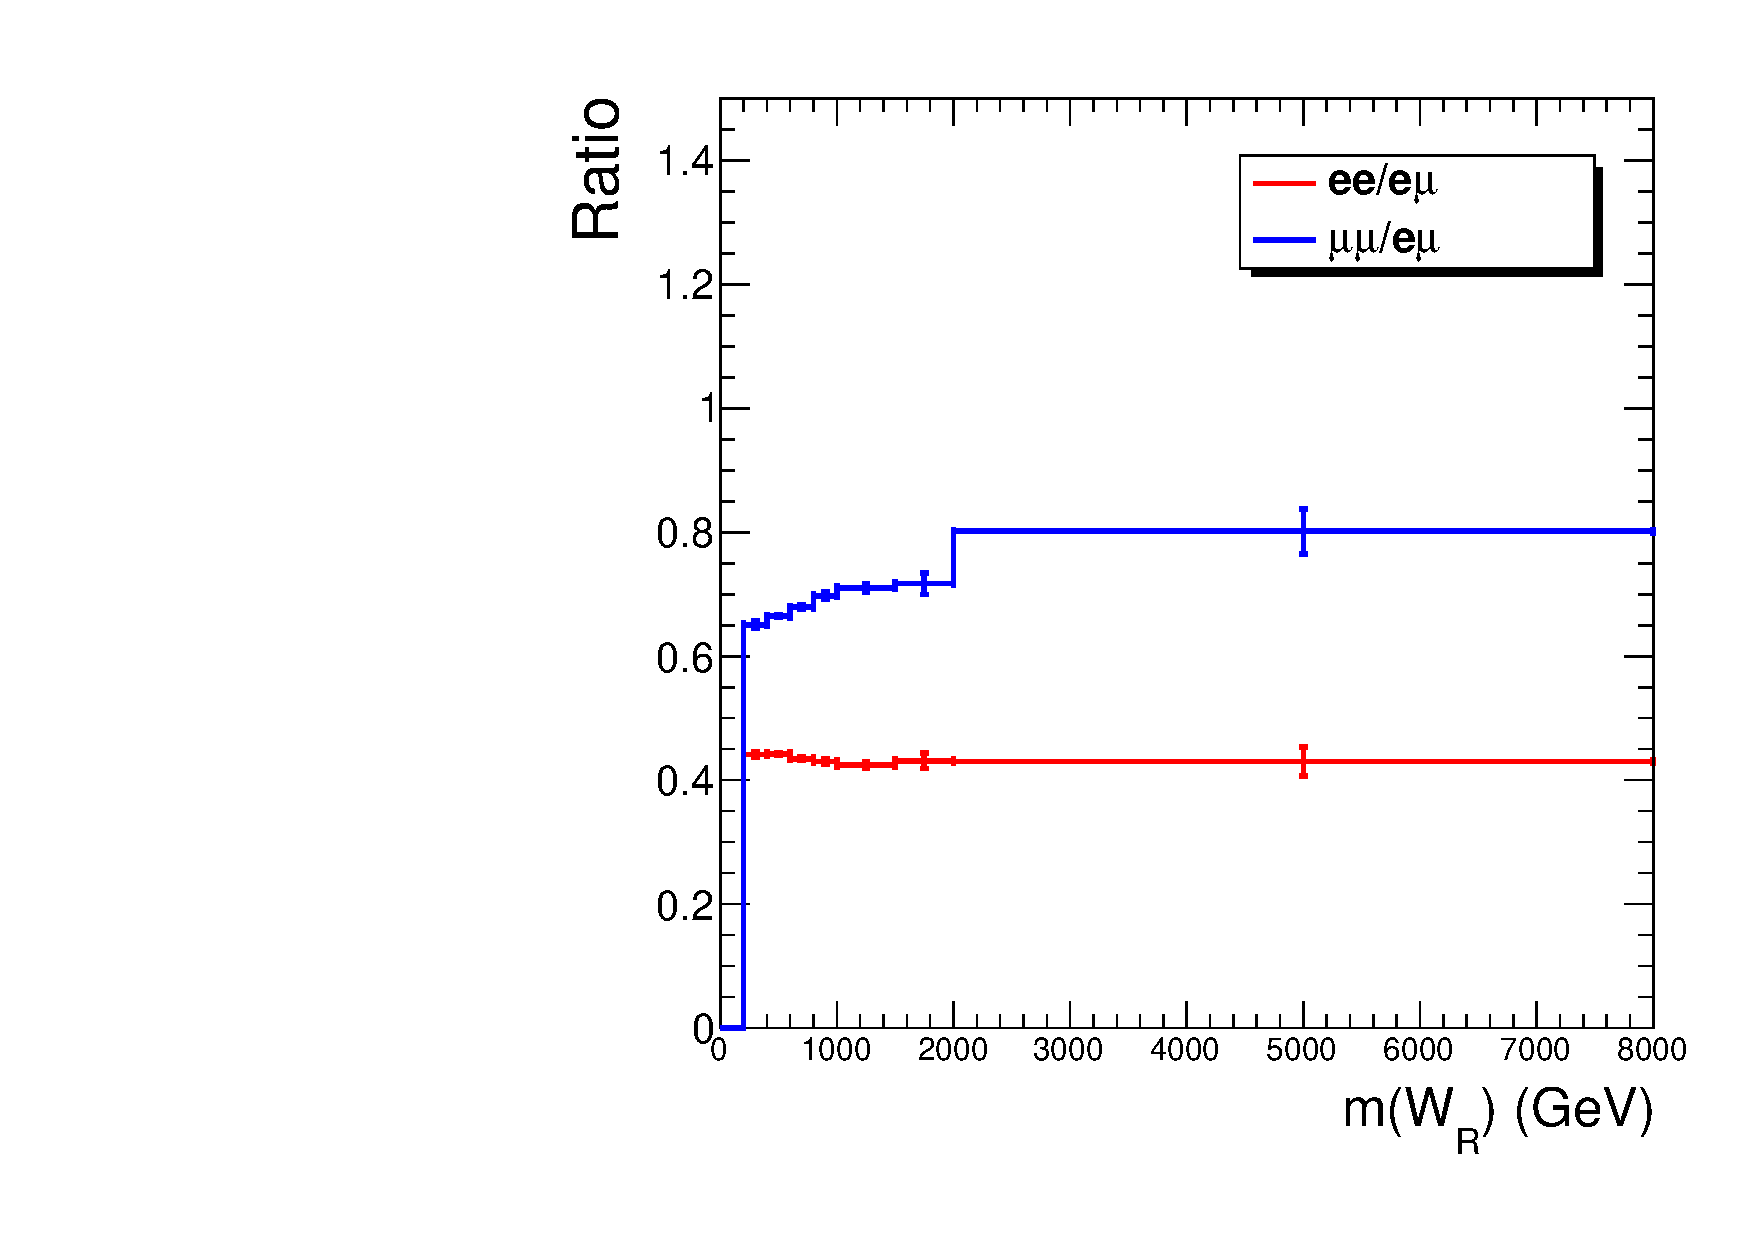
\includegraphics[width=0.45\textwidth]{figures/2016/Ratios_Resolved_WRCand_Mass_TTLX_powheg.pdf}
  \vspace{0.01\textwidth}

  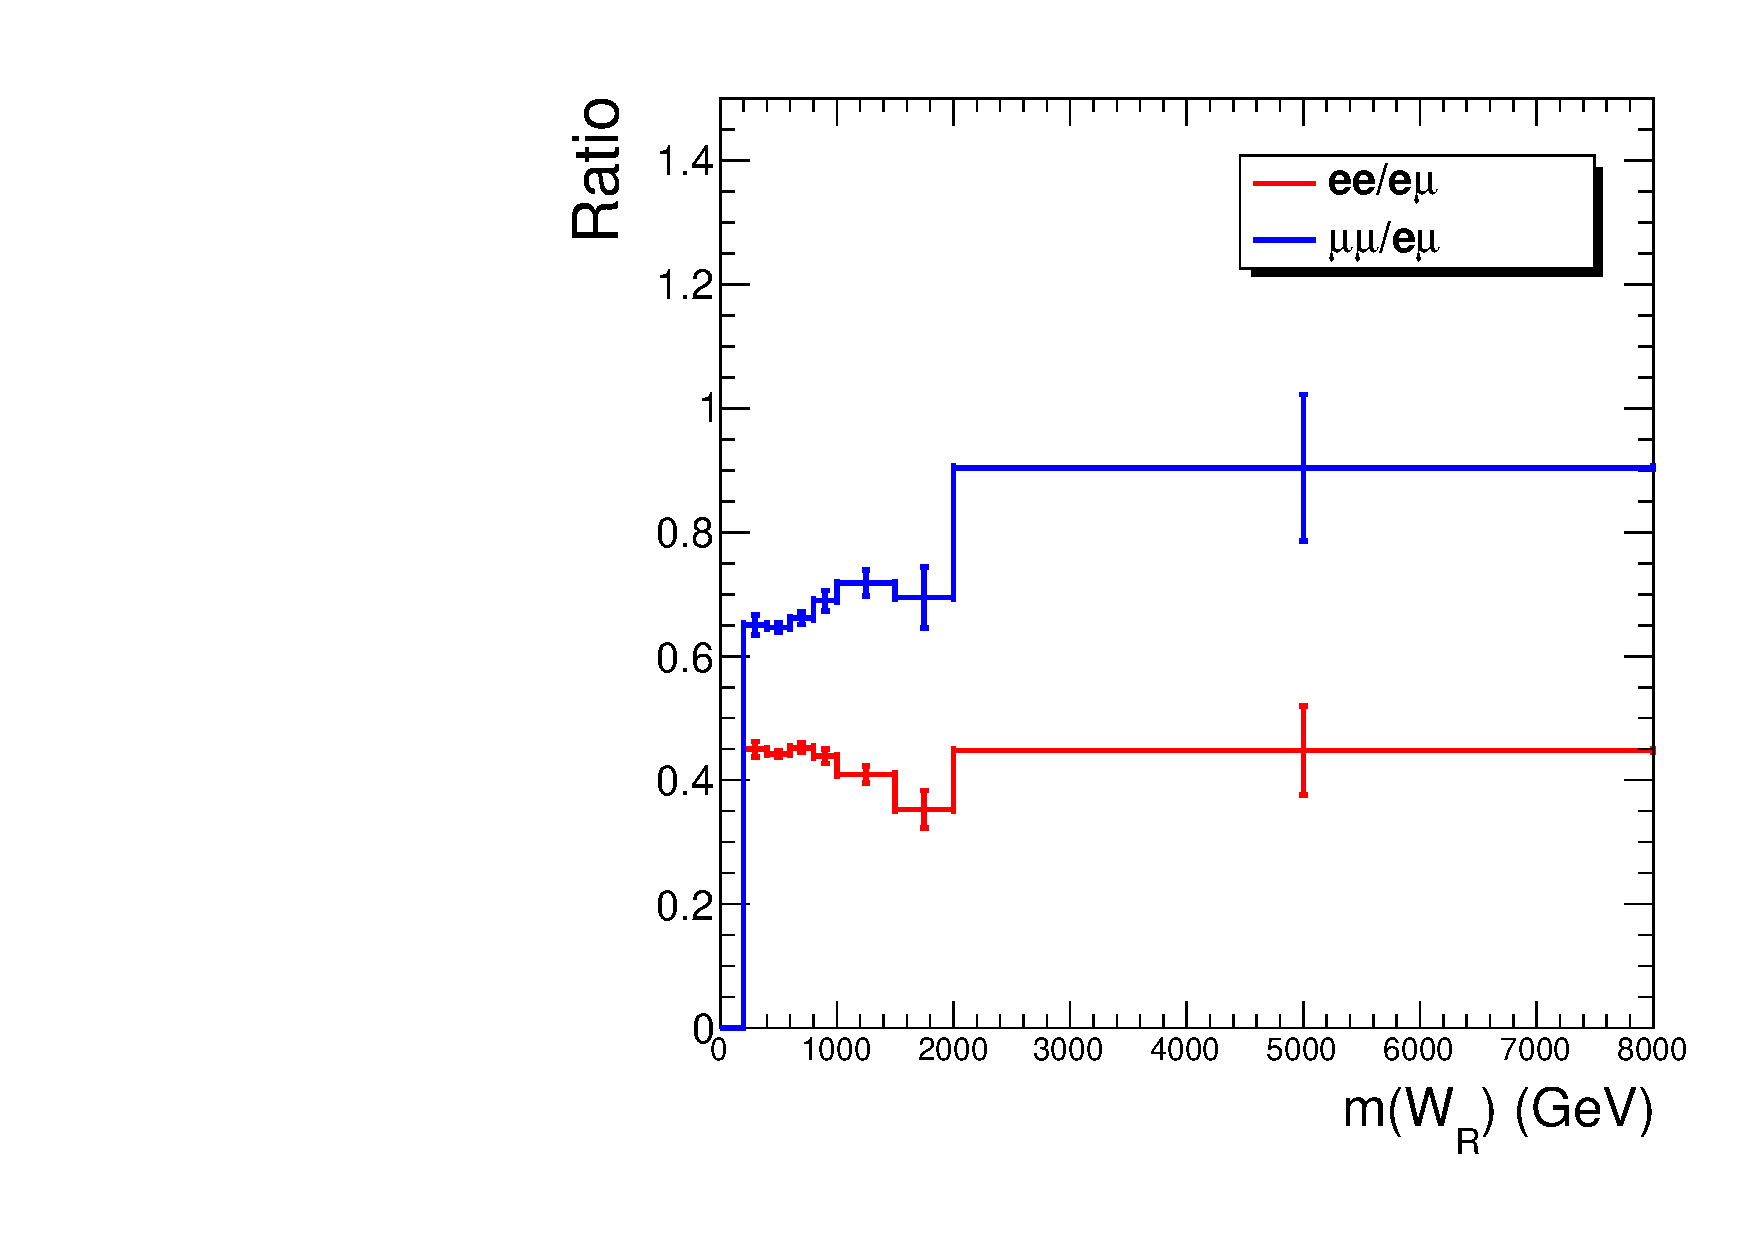
\includegraphics[width=0.45\textwidth]{figures/2017/Ratios_Resolved_WRCand_Mass_TTLX_powheg.pdf}
  \vspace{0.01\textwidth}

  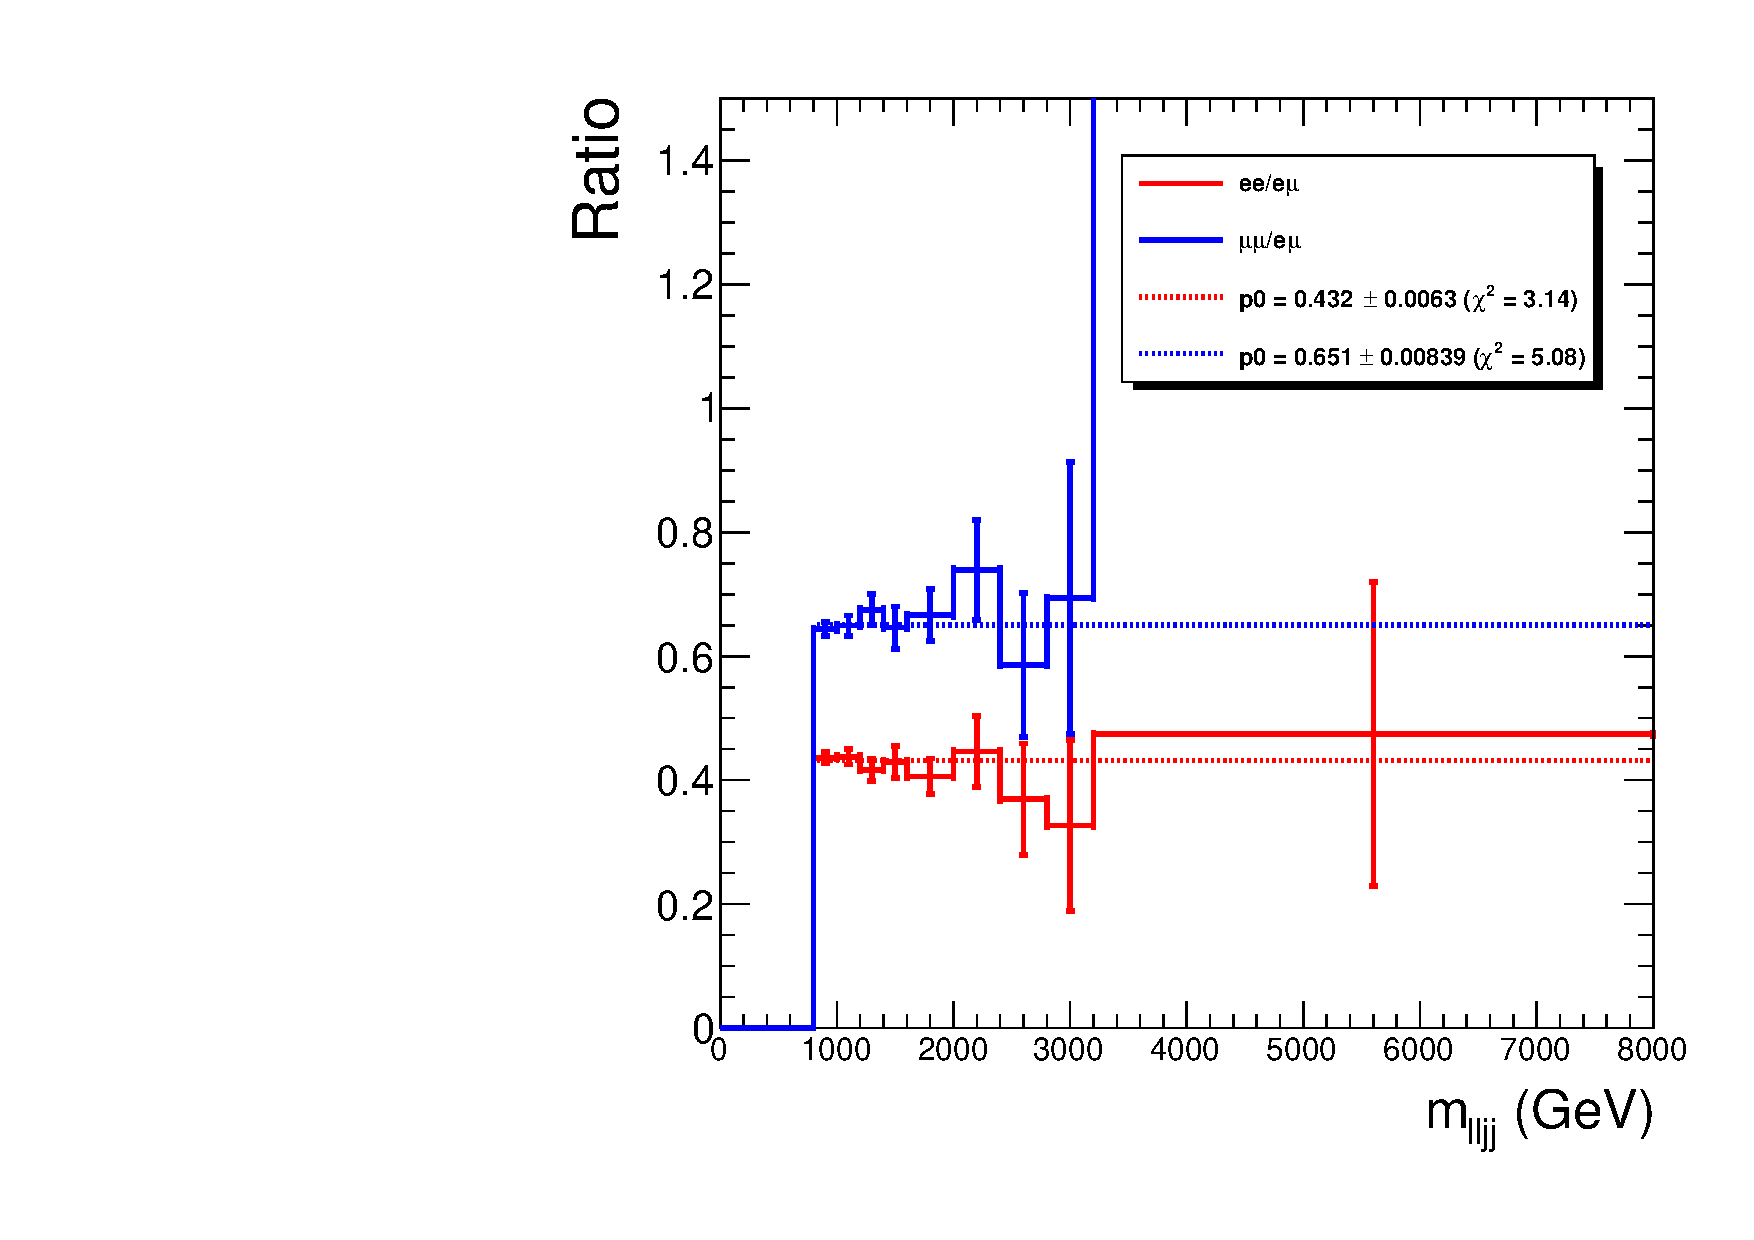
\includegraphics[width=0.45\textwidth]{figures/2018/Ratios_Resolved_WRCand_Mass_TTLX_powheg.pdf}

  \topcaption{
    The signal region to $\Pe\mu$-sideband ratio as a function of the mass of $\PWR$ in the resolved category, for 2016 (left), 2017 (middle) and 2018 (right).
  }
  \label{fig:emuRatioResolved}
\end{figure}

\begin{figure}[htbp]
  \centering

  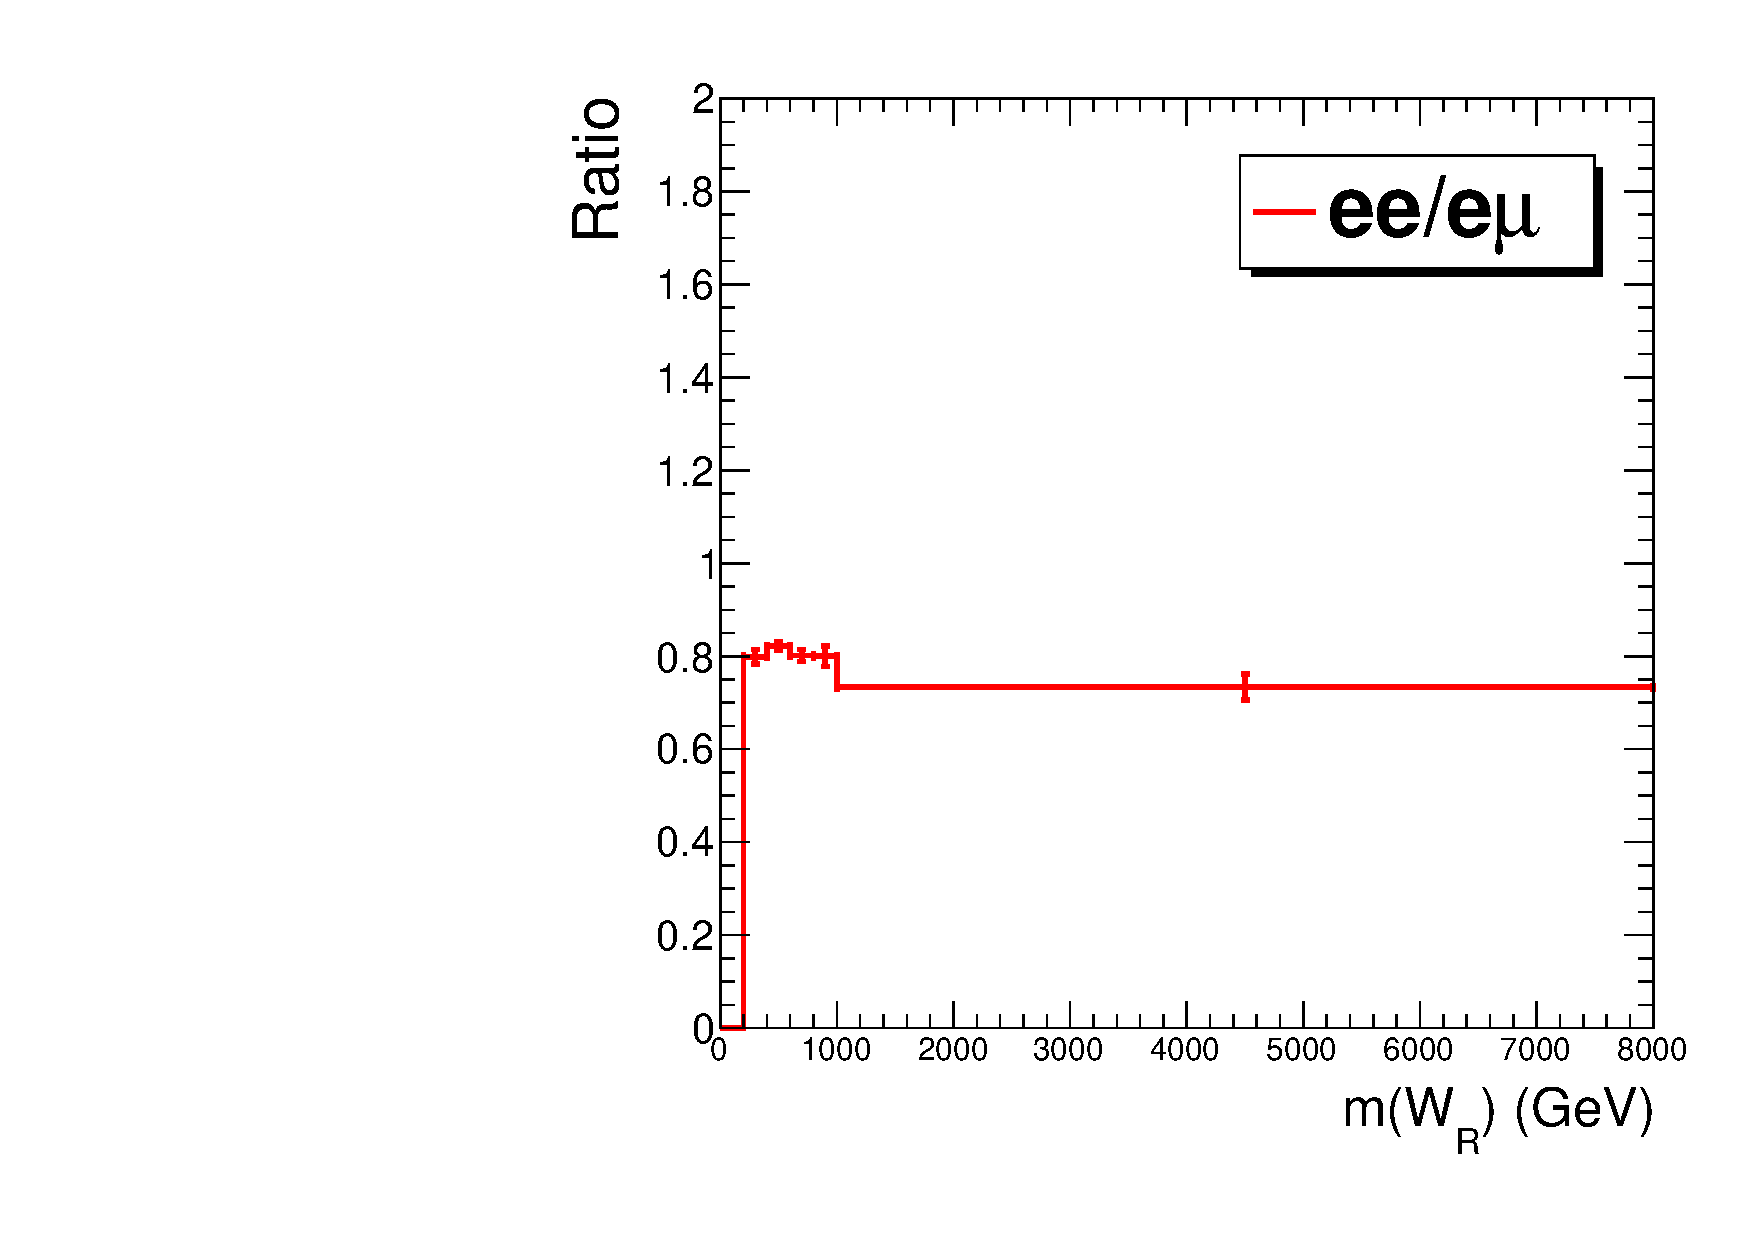
\includegraphics[width=0.45\textwidth]{figures/2016/Ratios_Boosted_elFatJet_WRCand_Mass_TTLX_powheg.pdf}
  \hspace{0.01\textwidth}
  \includegraphics[width=0.45\textwidth]{figures/2016/Ratios_Boosted_muFatJet_WRCand_Mass_TTLX_powheg.pdf}
  \vspace{0.01\textwidth}

  \includegraphics[width=0.45\textwidth]{figures/2017/Ratios_Boosted_elFatJet_WRCand_Mass_TTLX_powheg.pdf}
  \hspace{0.01\textwidth}
  \includegraphics[width=0.45\textwidth]{figures/2017/Ratios_Boosted_muFatJet_WRCand_Mass_TTLX_powheg.pdf}
  
 \includegraphics[width=0.45\textwidth]{figures/2018/Ratios_Boosted_elFatJet_WRCand_Mass_TTLX_powheg.pdf}
  \hspace{0.01\textwidth}
  \includegraphics[width=0.45\textwidth]{figures/2018/Ratios_Boosted_muFatJet_WRCand_Mass_TTLX_powheg.pdf}

  \topcaption{
    The signal region to $\Pe\mu$-sideband ratio as a function of the mass of $\PWR$ in the boosted category.
    Results with the events containing $\Pe$--jet ($\mu$--jet) are on the left (right), for 2016 (top), 2017 (middle) and 2018 (bottom).
  }
  \label{fig:emuRatioBoosted}
\end{figure}

\begin{figure}[htbp]
  \centering

  \includegraphics[width=0.45\textwidth]{figures/2016/WRCand_Mass_HNWR_EMu_Resolved_SR.pdf}
  \vspace{0.01\textwidth}

  \includegraphics[width=0.45\textwidth]{figures/2017/WRCand_Mass_HNWR_EMu_Resolved_SR.pdf}
  \vspace{0.01\textwidth}

  \includegraphics[width=0.45\textwidth]{figures/2018/WRCand_Mass_HNWR_EMu_Resolved_SR.pdf}

  \topcaption{
    The reconstructed mass of $\PWR$ in the resolved signal region, for 2016 (left), 2017 (middle) and 2018 (right).
  }
  \label{fig:emuDATAMCResolved}
\end{figure}


\begin{table}[htb]
  \centering
  \topcaption{
    The fit results of the $\Pe\mu$--ratios, with the statistical uncertainties.
  }
  \begin{tabular}{ccccc}
\hline
\multirow{2}{*}{Year} & \multicolumn{2}{c}{Resolved} & \multicolumn{2}{c}{Boosted} \\
                      & $\Pe\Pe$ & $\mu\mu$ & $\Pe\Pe$ & $\mu\mu$ \\
\hline
2016                  & $0.438 \pm 0.001$ & $0.674 \pm 0.002$ & $0.808 \pm 0.006$ & $1.246 \pm 0.010$ \\
2017                  & $0.441 \pm 0.004$ & $0.660 \pm 0.005$ & $0.835 \pm 0.018$ & $1.209 \pm 0.029$ \\
2018                  & $0.436 \pm 0.001$ & $0.650 \pm 0.002$ & $0.827 \pm 0.008$ & $1.226 \pm 0.013$ \\
\hline
  \end{tabular}
  \label{tab:EMuRatioFit}
\end{table}


\begin{figure}[htbp]
  \centering

  \includegraphics[width=0.45\textwidth]{figures/2016/WRCand_Mass_HNWR_SingleMuon_EMu_Boosted_CR.pdf}
  \hspace{0.01\textwidth}
  \includegraphics[width=0.45\textwidth]{figures/2016/leadAK8JetElectronMass.png}
  \vspace{0.01\textwidth}

  \includegraphics[width=0.45\textwidth]{figures/2017/WRCand_Mass_HNWR_SingleMuon_EMu_Boosted_CR.pdf}
  \hspace{0.01\textwidth}
  \includegraphics[width=0.45\textwidth]{figures/2017/leadAK8JetElectronMass.png}
  
  \includegraphics[width=0.45\textwidth]{figures/2018/WRCand_Mass_HNWR_SingleMuon_EMu_Boosted_CR.pdf}
  \hspace{0.01\textwidth}
  \includegraphics[width=0.45\textwidth]{figures/2018/leadAK8JetElectronMass.png}


  \topcaption{
    The reconstructed mass of $\PWR$ in the boosted signal region.
    Results with the events containing $\Pe$--jet ($\mu$--jet) are on the left (right), for 2016 (top), 2017 (middle) and 2018 (bottom).
  }
  \label{fig:emuDATAMCBoosted}
\end{figure}

\begin{figure}[htbp]
  \centering

  \includegraphics[width=0.45\textwidth]{figures/2016/Resolved_WRCand_Mass_HNWR_SingleElectron_Resolved_SR_TTLX_powheg.pdf}
  \hspace{0.01\textwidth}
  \includegraphics[width=0.45\textwidth]{figures/2016/Resolved_WRCand_Mass_HNWR_SingleMuon_Resolved_SR_TTLX_powheg.pdf}
  \vspace{0.01\textwidth}

  \includegraphics[width=0.45\textwidth]{figures/2017/Resolved_WRCand_Mass_HNWR_SingleMuon_Resolved_SR_TTLX_powheg.pdf}
  \hspace{0.01\textwidth}
  \includegraphics[width=0.45\textwidth]{figures/2017/Resolved_WRCand_Mass_HNWR_SingleMuon_Resolved_SR_TTLX_powheg.pdf}
  
  \includegraphics[width=0.45\textwidth]{figures/2018/Resolved_WRCand_Mass_HNWR_SingleMuon_Resolved_SR_TTLX_powheg.pdf}
  \hspace{0.01\textwidth}
  \includegraphics[width=0.45\textwidth]{figures/2018/Resolved_WRCand_Mass_HNWR_SingleMuon_Resolved_SR_TTLX_powheg.pdf}


  \topcaption{
    The \ttbar contribution to the reconstructed mass of $\PWR$ in the resolved signal region.
    Result from MC (Data-driven) are drawn in the black marker (orange histogram).
    Results for dielectron (dimuon) channel is shown on the left (right), for 2016 (top), 2017 (middle) and 2018 (bottom).
  }
  \label{fig:emuMCEMuCompResolved}
\end{figure}

\begin{figure}[htbp]
  \centering

  \includegraphics[width=0.45\textwidth]{figures/2016/Boosted_elFatJet_WRCand_Mass_HNWR_SingleElectron_Boosted_SR_TTLX_powheg.pdf}
  \hspace{0.01\textwidth}
  \includegraphics[width=0.45\textwidth]{figures/2016/Boosted_muFatJet_WRCand_Mass_HNWR_SingleMuon_Boosted_SR_TTLX_powheg.pdf}
  \vspace{0.01\textwidth}

  \includegraphics[width=0.45\textwidth]{figures/2017/Boosted_elFatJet_WRCand_Mass_HNWR_SingleElectron_Boosted_SR_TTLX_powheg.pdf}
  \hspace{0.01\textwidth}
  \includegraphics[width=0.45\textwidth]{figures/2017/Boosted_muFatJet_WRCand_Mass_HNWR_SingleMuon_Boosted_SR_TTLX_powheg.pdf}

  \includegraphics[width=0.45\textwidth]{figures/2018/Boosted_elFatJet_WRCand_Mass_HNWR_SingleElectron_Boosted_SR_TTLX_powheg.pdf}
  \hspace{0.01\textwidth}
  \includegraphics[width=0.45\textwidth]{figures/2018/Boosted_muFatJet_WRCand_Mass_HNWR_SingleMuon_Boosted_SR_TTLX_powheg.pdf}

  \topcaption{
    The \ttbar contribution to the reconstructed mass of $\PWR$ in the boosted signal region.
    Result from MC (Data-driven) are drawn in the black marker (orange histogram).
    Results for dielectron (dimuon) channel is shown on the left (right), for 2016 (top), 2017 (middle) and 2018 (bottom).
  }
  \label{fig:emuMCEMuCompBoosted}
\end{figure}


For the systematic uncertainty on the scale factors, a closure test is performed in the low invariant mass region for both analyses.
The largest discrepancy between the background prediction and the data is used as a systematic uncertainty.
{\color{red}TO DO evaluate uncertainties}

